% -*- root: main.tex -*-
\appendix{}
\label{sec:appendix}

\subsection*{Detailed Precision and Recall Values}

In Section~\ref{sec:case_study_results}, we presented the F1-measures for all projects when answering our RQs. In this appendix, we added the detailed precision and recall values that make up the F1-measures.


\begin{table}[h]
  \begin{minipage}{\textwidth}
    \begin{center}
        \caption{Detailed Comparison of F1-measure Between the NLP-based, the Comment Patterns and the Random Baseline Approaches for Design Debt}
        \label{tbl:classifier_results_vs_baseline_design}
        \begin{tabular}{l| c c c|| c c c|| c c c}
        \toprule

        \multirow{4}{*}{\textbf{\thead{Project}}} & \multicolumn{3}{c||}{\textbf{\thead{NLP-based}}} & \multicolumn{3}{c||}{\textbf{\thead{Comment Patterns}}} & \multicolumn{3}{c}{\textbf{\thead{Random Baseline}}} 
        
        \\ 
        \cmidrule{2-10}
        
        & \textbf{\thead{Precision}} & \textbf{\thead{Recall}} & \textbf{\thead{F1 measure}} & \textbf{\thead{Precision}} & \textbf{\thead{Recall}} & \textbf{\thead{F1 measure}} & \textbf{\thead{Precision}} & \textbf{\thead{Recall}} & \textbf{\thead{F1 measure}}\\
        \midrule
        \textbf{Ant}           &   0.554 &   0.484 &  0.517 &  0.608 & 0.147 & 0.237 &  0.024 & 0.5 & 0.045 \\
        \textbf{ArgoUML}       &   0.788 &   0.843 &  0.814 &  0.793 & 0.057 & 0.107 &  0.092 & 0.5 & 0.155 \\
        \textbf{Columba}       &   0.792 &   0.484 &  0.601 &  0.800 & 0.158 & 0.264 &   0.02 & 0.5 & 0.038 \\
        \textbf{EMF}           &   0.574 &   0.397 &  0.470 &  0.647 & 0.141 & 0.231 &  0.018 & 0.5 & 0.035 \\
        \textbf{Hibernate}     &   0.877 &   0.645 &  0.744 &  0.920 & 0.129 & 0.227 &  0.136 & 0.5 & 0.214 \\
        \textbf{JEdit}         &   0.779 &   0.378 &  0.509 &  0.857 & 0.214 & 0.342 &  0.019 & 0.5 & 0.037 \\
        \textbf{JFreeChart}    &   0.646 &   0.397 &  0.492 &  0.507 & 0.195 & 0.282 &  0.043 & 0.5 &  0.08 \\
        \textbf{Jmeter}        &   0.808 &   0.668 &  0.731 &  0.813 & 0.110 & 0.194 &   0.04 & 0.5 & 0.075 \\
        \textbf{JRuby}         &   0.798 &   0.770 &  0.783 &  0.864 & 0.483 & 0.620 &  0.075 & 0.5 & 0.131 \\
        \textbf{SQuirrel}      &   0.544 &   0.536 &  0.540 &  0.700 & 0.100 & 0.175 &   0.03 & 0.5 & 0.056 \\
        \bottomrule
        \end{tabular}
    \end{center}
  \end{minipage}    
\end{table}
                 

\begin{table}[h]
  \begin{minipage}{\textwidth}
    \begin{center}
        \caption{Detailed Comparison of F1-measure Between the NLP-based, the Comment Patterns and the Random Baseline Approaches for Requirement Debt}
        \label{tbl:classifier_results_vs_baseline_requirement}
        \begin{tabular}{l| c c c|| c c c|| c c c}
        \toprule

        \multirow{4}{*}{\textbf{\thead{Project}}} & \multicolumn{3}{c||}{\textbf{\thead{NLP-based}}} & \multicolumn{3}{c||}{\textbf{\thead{Comment Patterns}}} & \multicolumn{3}{c}{\textbf{\thead{Random Baseline}}} 
        
        \\ 
        \cmidrule{2-10}
        
        & \textbf{\thead{Precision}} & \textbf{\thead{Recall}} & \textbf{\thead{F1 measure}} & \textbf{\thead{Precision}} & \textbf{\thead{Recall}} & \textbf{\thead{F1 measure}} & \textbf{\thead{Precision}} & \textbf{\thead{Recall}} & \textbf{\thead{F1 measure}}\\
        \midrule
        \textbf{Ant}           &  0.154 & 0.154 &  0.154 & 0.000  &  0.000   & 0.000  & 0.003 &  0.5 &  0.006 \\
        \textbf{ArgoUML}       &  0.663 & 0.540 &  0.595 & 0.000  &  0.000   & 0.000  & 0.045 &  0.5 &  0.083 \\
        \textbf{Columba}       &  0.755 & 0.860 &  0.804 & 0.375  &  0.069   & 0.117  & 0.007 &  0.5 &  0.013 \\
        \textbf{EMF}           &  0.800 & 0.250 &  0.381 & 0.000  &  0.000   & 0.000  & 0.004 &  0.5 &  0.007 \\
        \textbf{Hibernate}     &  0.610 & 0.391 &  0.476 & 0.000  &  0.000   & 0.000  & 0.022 &  0.5 &  0.042 \\
        \textbf{JEdit}         &  0.125 & 0.071 &  0.091 & 0.000  &  0.000   & 0.000  & 0.001 &  0.5 &  0.003 \\
        \textbf{JFreeChart}    &  0.220 & 0.600 &  0.321 & 0.102  &  0.266   & 0.148  & 0.003 &  0.5 &  0.007 \\
        \textbf{Jmeter}        &  0.153 & 0.524 &  0.237 & 0.000  &  0.000   & 0.000  & 0.003 &  0.5 &  0.005 \\
        \textbf{JRuby}         &  0.686 & 0.318 &  0.435 & 0.573  &  0.318   & 0.409  & 0.023 &  0.5 &  0.044 \\
        \textbf{SQuirrel}      &  0.657 & 0.460 &  0.541 & 0.000  &  0.000   & 0.000  & 0.007 &  0.5 &  0.014 \\
        \bottomrule
        \end{tabular}
    \end{center}
  \end{minipage}    
\end{table}

% \clearpage

% \begin{table}
%     \begin{center}
%         \caption{Technical Debt distribution per type}
%         \label{tbl:td_distribution}
%         \begin{tabular}{l|ccccccc}
%         \toprule
%         \multirow{2}{*}{Project} & \multicolumn{3}{c}{TD Distribution} \\ & {Design} & {Req.}  & {Other} & \multirow{-2}{*}{Total TD comments} & \multirow{-2}{*}{Total comments} &  \multirow{-2}{*}{TD \%} \\
%         \midrule
%         Ant            &  95 &  13  &  23 &   131 &   4,137  & 03.1 \\
%         ArgoUML        &  801 & 411 & 201 & 1.413 &   9,548  & 14.7 \\
%         Columba        &  126 &  43 &  35 &   204 &   6,478  & 03.1 \\
%         EMF            &  78 &  16  &  10 &   104 &   4,401  & 02.3 \\
%         Hibernate      &  355 &  64 &  53 &   472 &   2,968  & 15.9 \\
%         JEdit          &  196 &  14 &  46 &   256 &  10,322  & 02.4 \\
%         JFreeChart     &  184 &  15 &  10 &   209 &   4,423  & 04.7 \\
%         Jmeter         &  316 &  21 &  37 &   374 &   8,162  & 04.5 \\
%         JRuby          &  343 & 110 & 169 &   622 &   4,897  & 12.7 \\
%         SQuirrel       &  209 & 50  & 27  &   286 &   7,230  & 03.9 \\
%         \bottomrule
%         \end{tabular}
%     \end{center}    
% \end{table}



% \clearpage

% \begin{table}[!hbt]
%     \begin{center}
%         \caption{Design Debt features per project}
%         \label{tbl:design_features_per_project}
%         \begin{tabular}{l| c c c }
%         \toprule
%         \textbf{Project} & \thead{Positive\\Design TD\\Features} & \thead{Negative\\Design TD\\Features} & \thead{Total\\Features} \\
%         \midrule
%         Ant          &5,299 & 23,623 &28,922 \\
%         ArgoUML      &3,917 & 26,012 &29,929 \\
%         Columba      &5,255 & 24,182 &29,437 \\
%         EMF          &5,346 & 23,667 &29,013 \\
%         Hibernate    &4,914 & 24,070 &28,984 \\
%         JEdit        &5,042 & 24,644 &29,686 \\
%         JFreeChart   &5,361 & 23,530 &28,891 \\
%         Jmeter       &5,172 & 23,916 &29,088 \\
%         JRuby        &4,856 & 24,553 &29,409 \\
%         SQuirrel     &4,982 & 25,146 &30,128 \\
%         \midrule
%         Average       & 5,014  & 24,334 & 29,348  \\      
%         Total unique  & 6,327  & 31,518 & 35,828  \\
%         \bottomrule
%         \end{tabular}
%     \end{center}    
% \end{table}

% \begin{table}[!hbt]
%     \begin{center}
%         \caption{Requirement Debt features per project}
%         \label{tbl:requirement_features_per_project}
%         \begin{tabular}{l| c c c }
%         \toprule
%         \textbf{Project} & \thead{Requirement TD\\features} & \thead{No TD\\Features} & \thead{Total\\Features} \\
%         \midrule
%         Ant           & 1,812 & 27,673 & 29,485  \\
%         ArgoUML       & 2,779 & 27,260 & 30,039  \\
%         Columba       & 2,433 & 27,561 & 29,994  \\
%         EMF           & 1,889 & 27,637 & 29,526  \\
%         Hibernate     & 2,748 & 26,654 & 29,402  \\
%         JEdit         & 1,831 & 28,267 & 30,098  \\
%         JFreeChart    & 1,902 & 27,439 & 29,341  \\
%         Jmeter        & 1,893 & 27,716 & 29,609  \\
%         JRuby         & 2,850 & 27,085 & 29,935  \\
%         SQuirrel      & 1,814 & 26,914 & 28,728  \\
%         \midrule
%         Average       & 2,195  & 27,420 & 29,615 \\      
%         Total unique  & 4,015  & 32,954 & 32,954 \\
%         \bottomrule
%         \end{tabular}
%     \end{center}    
% \end{table}

\clearpage

\subsection*{Investigating the Amount of Training Data Required vs. Classification Performance}

In Section~\ref{sec:case_study_results} (RQ3), we presented the Figures for Ant and ArogUML only. Here, we present the same Figures for all projects, for both, design and requirement \SATD.


\begin{figure}[thb!]
  \centering
  \vspace{-5mm}
  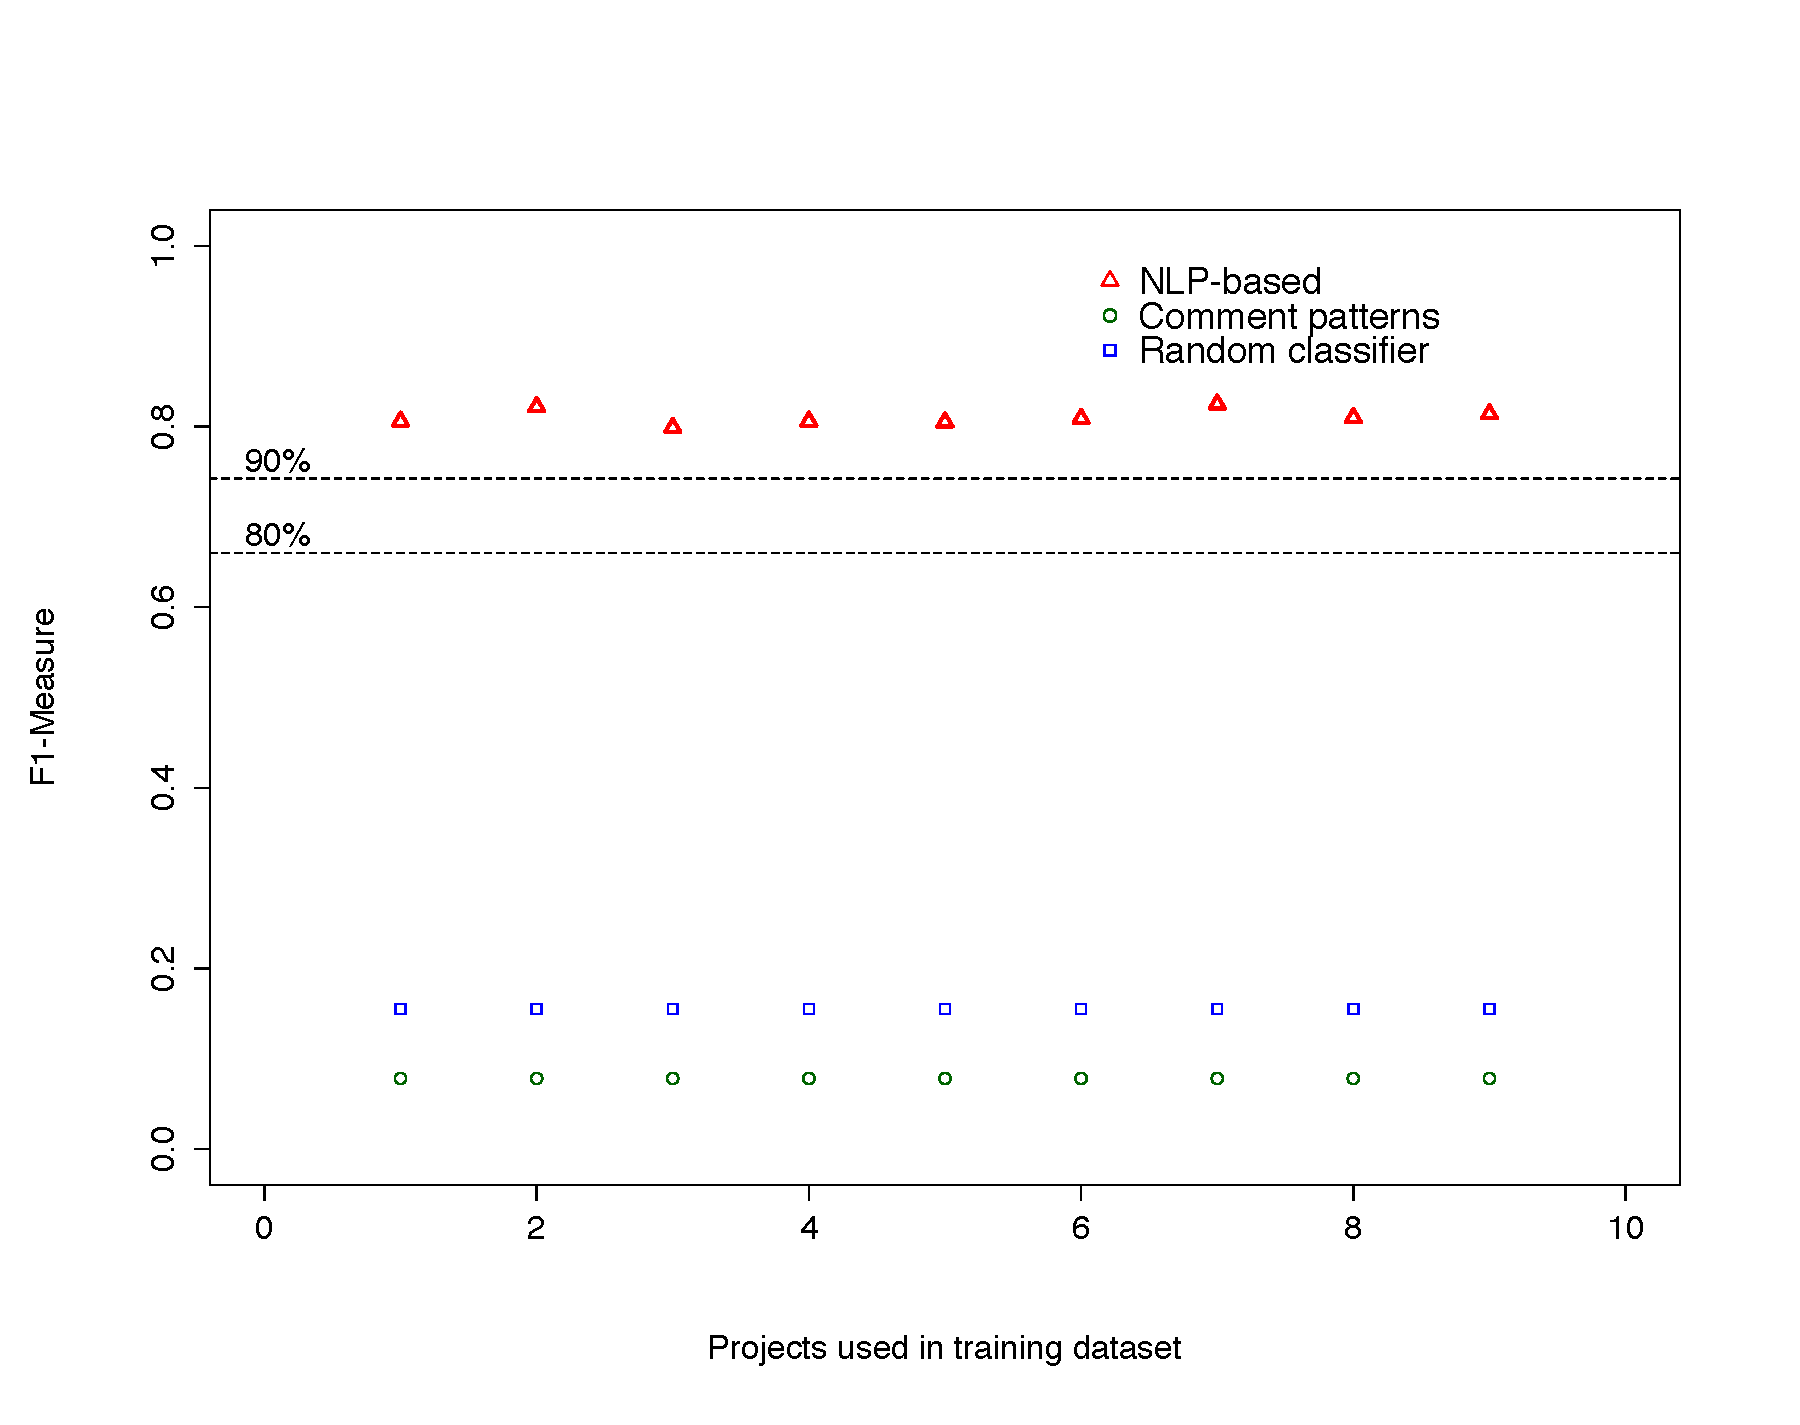
\includegraphics[width=0.49\textwidth]{figures/appendix/iteration_details/design_argo.pdf}
  \vspace{-9mm}
  \caption{Argo Design Debt Classification}
  \label{fig:design_argo}
  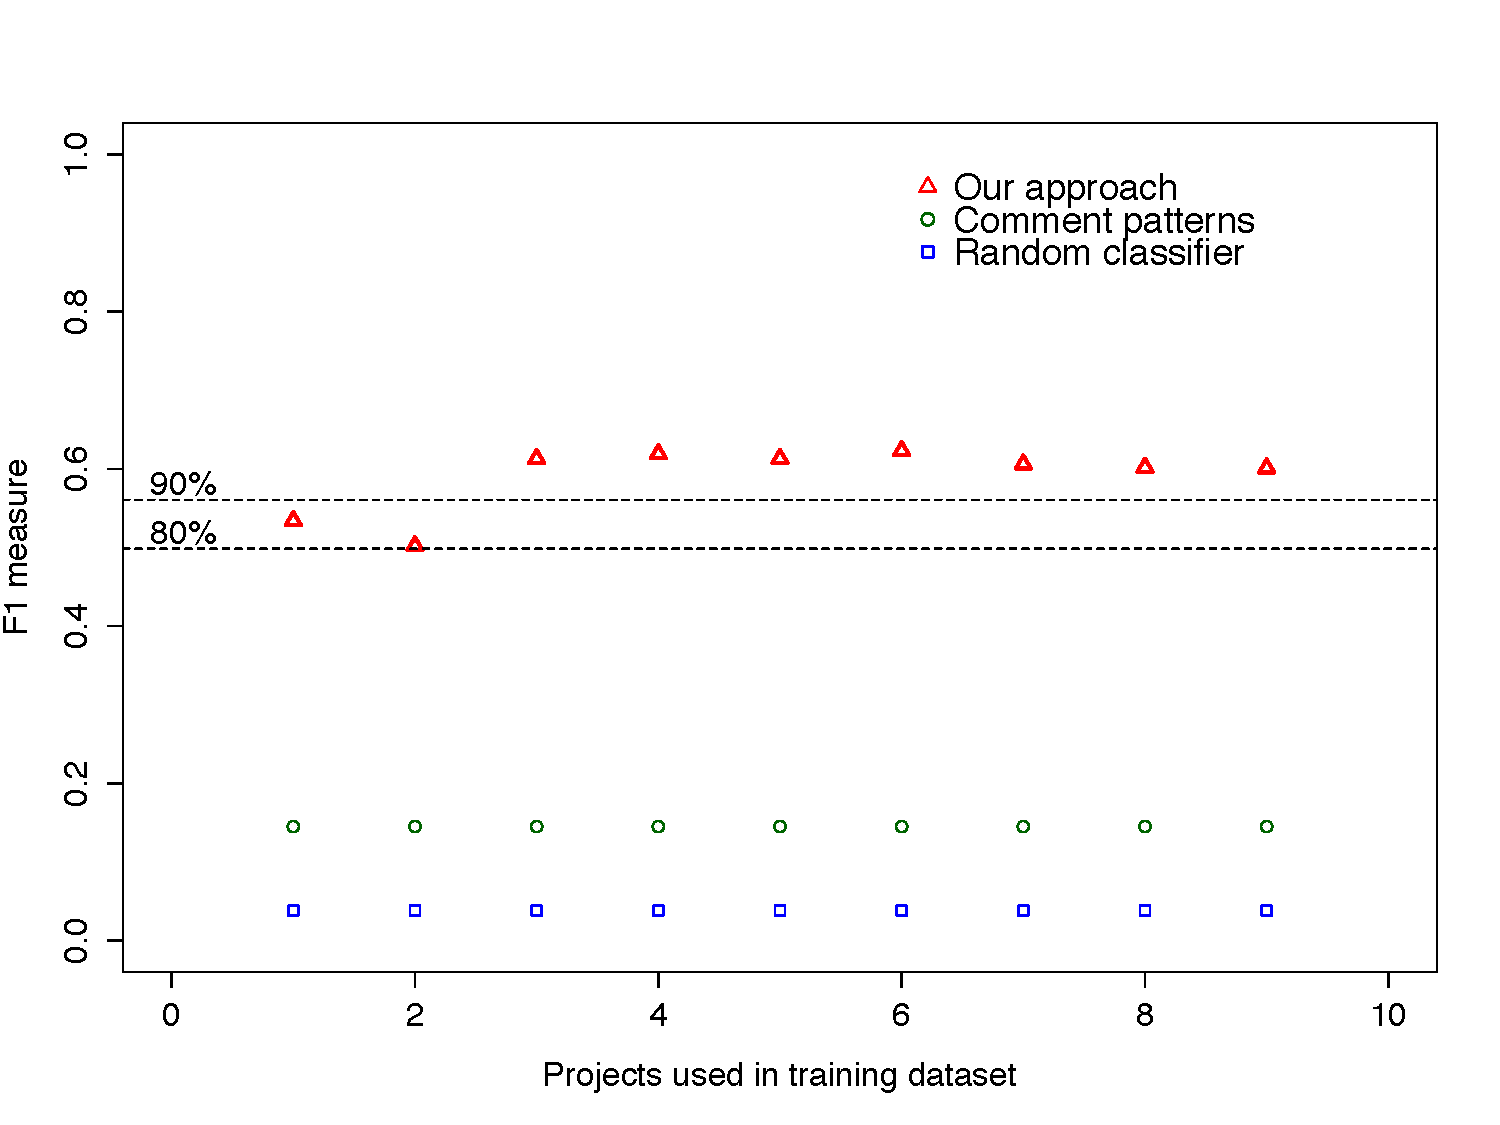
\includegraphics[width=0.49\textwidth]{figures/appendix/iteration_details/design_columba.pdf}
  \vspace{-9mm}
  \caption{Columba Design Debt Classification}
  \label{fig:design_columba}
  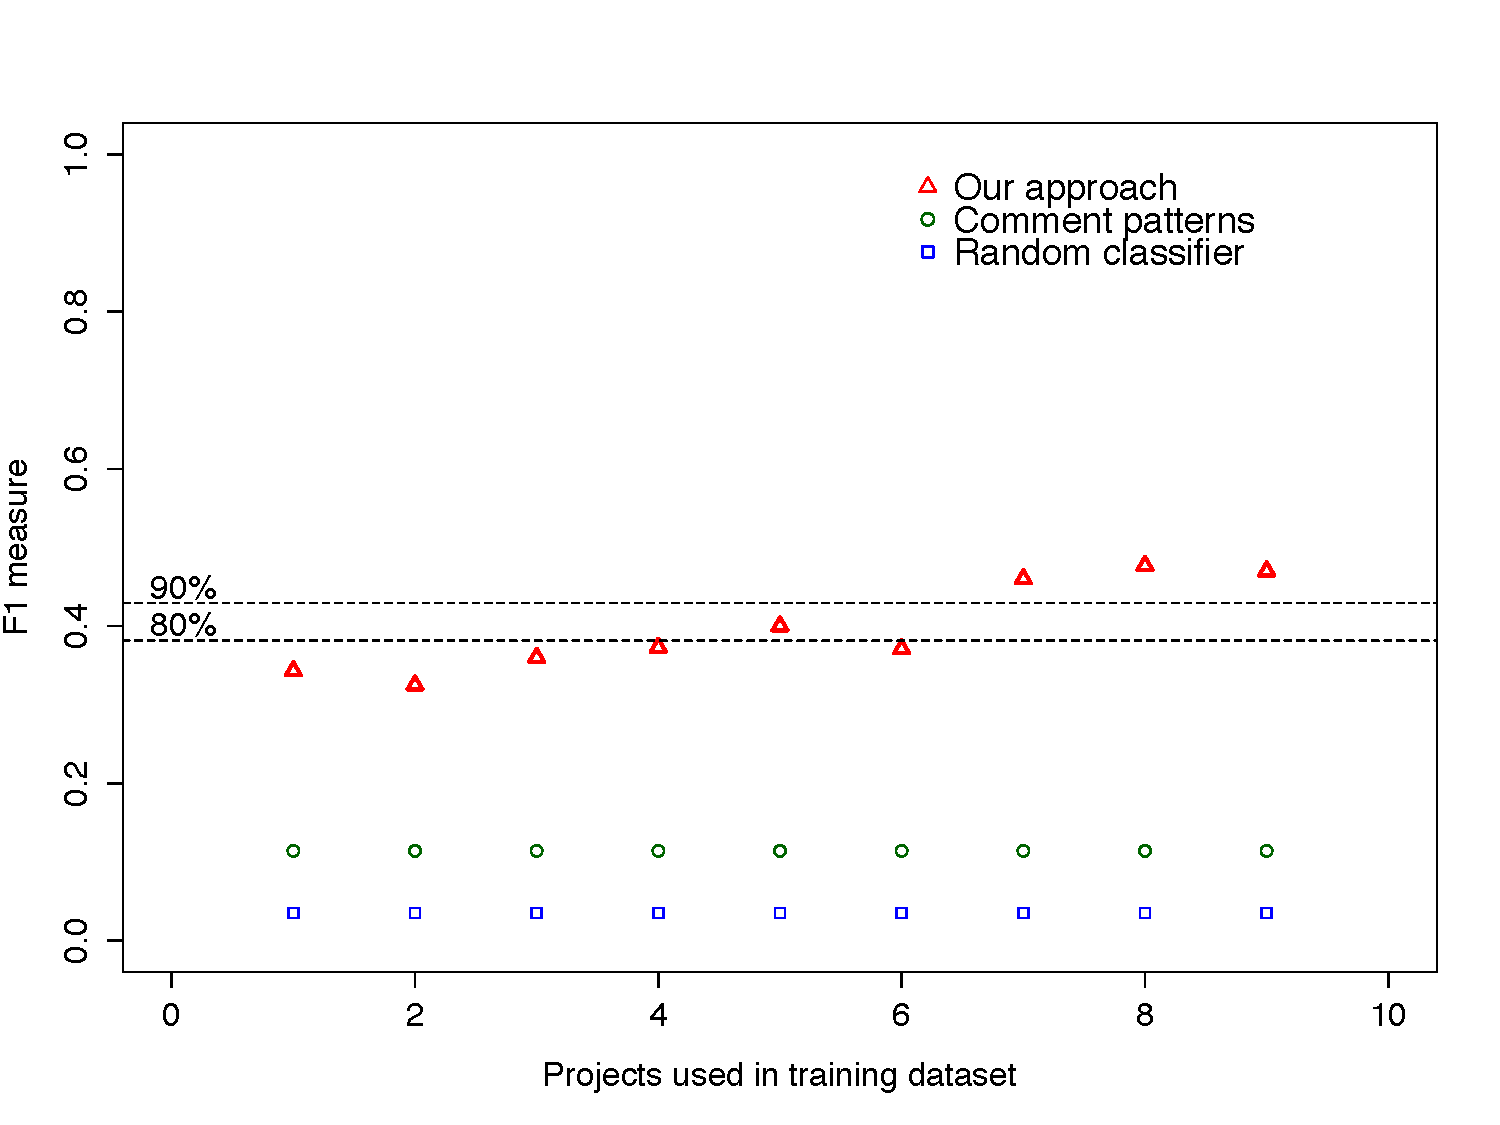
\includegraphics[width=0.49\textwidth]{figures/appendix/iteration_details/design_emf.pdf}
  \vspace{-9mm}
  \caption{Emf Design Debt Classification}
  \label{fig:design_emf}
\end{figure}

\begin{figure}[thb!]
  \centering
  \vspace{21mm}
  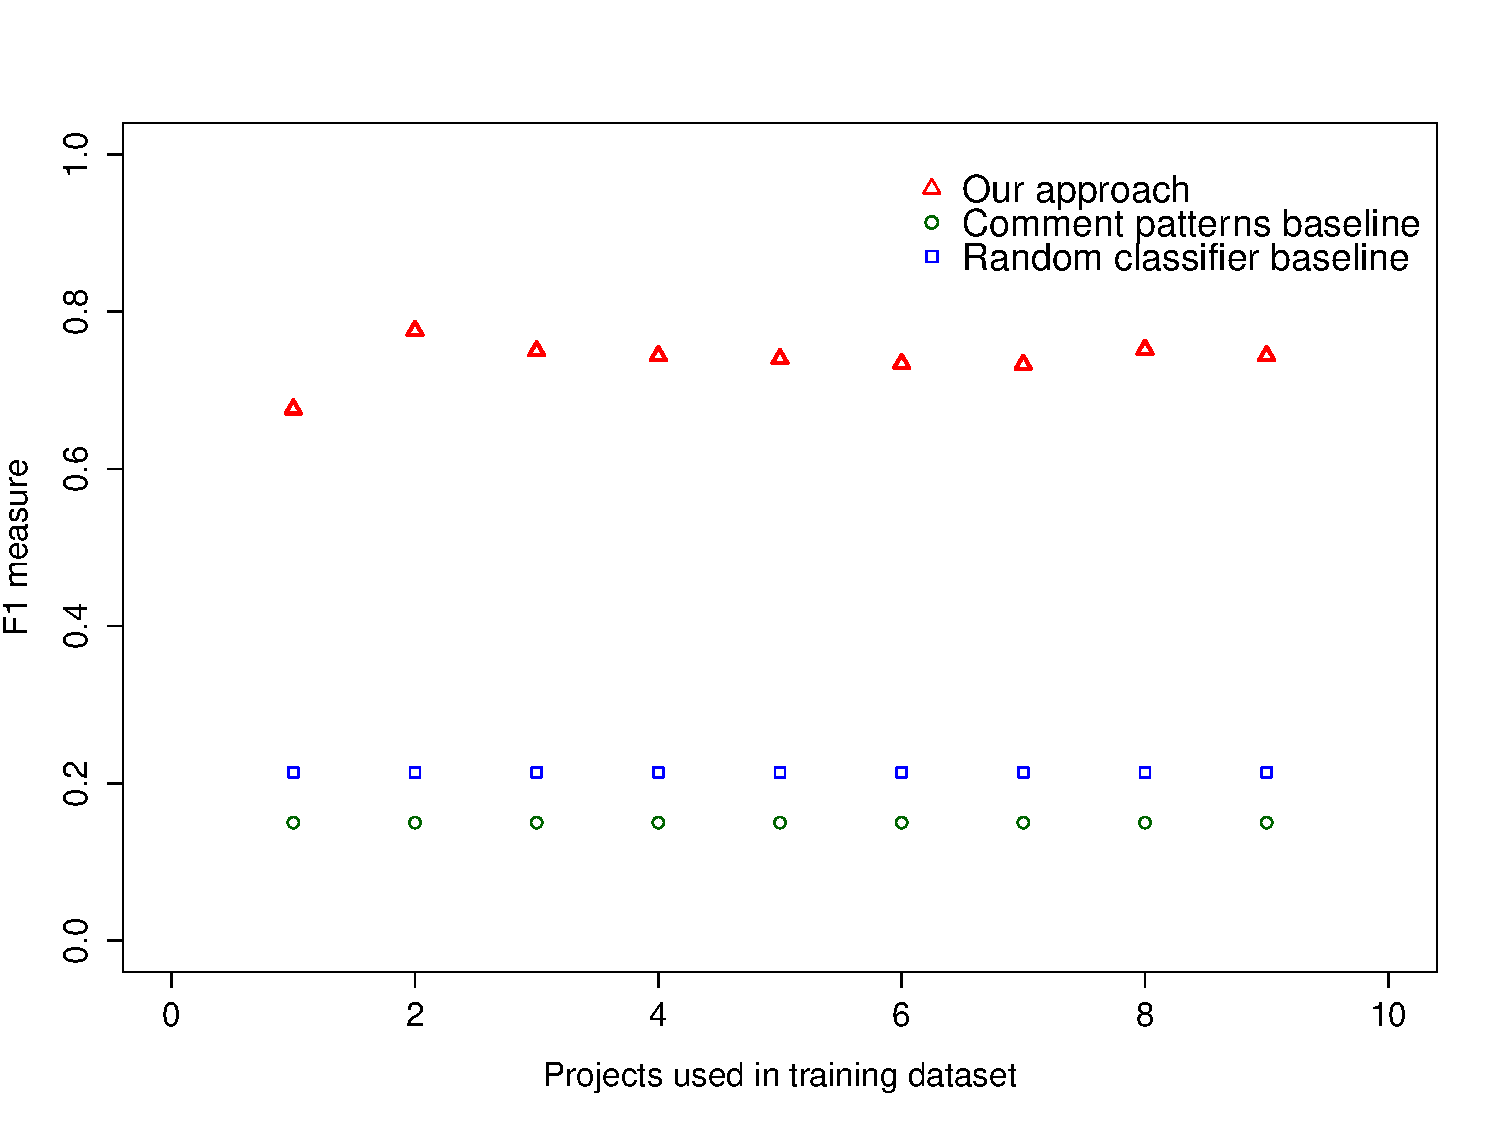
\includegraphics[width=0.49\textwidth]{figures/appendix/iteration_details/design_hibernate.pdf}
  \vspace{-9mm}
  \caption{Hibernate Design Debt Classification}
  \label{fig:design_hibernate}
  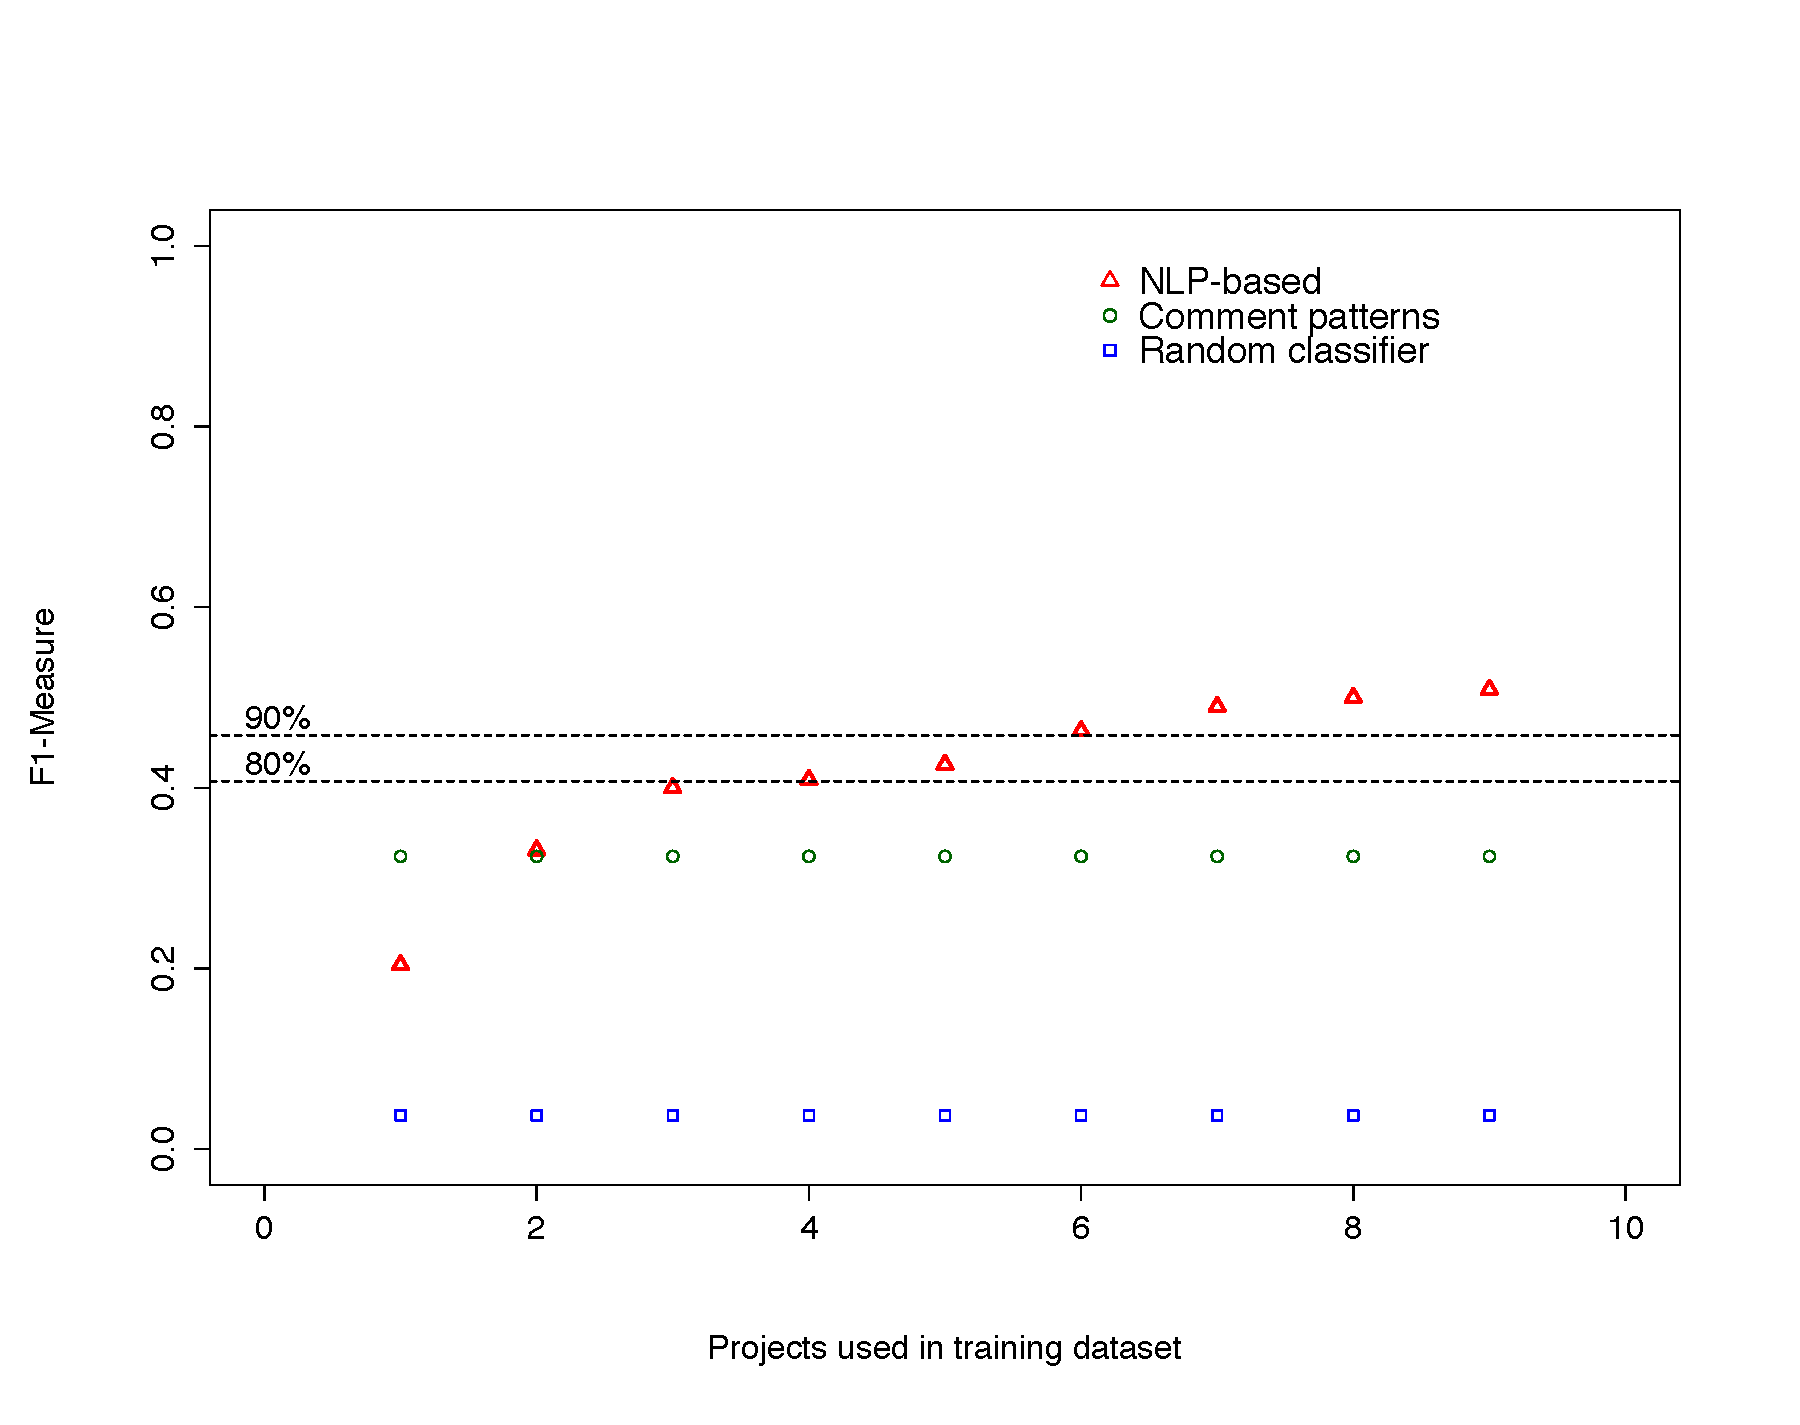
\includegraphics[width=0.49\textwidth]{figures/appendix/iteration_details/design_jedit.pdf}
  \vspace{-9mm}
  \caption{JEdit Design Debt Classification}
  \label{fig:design_jedit}
  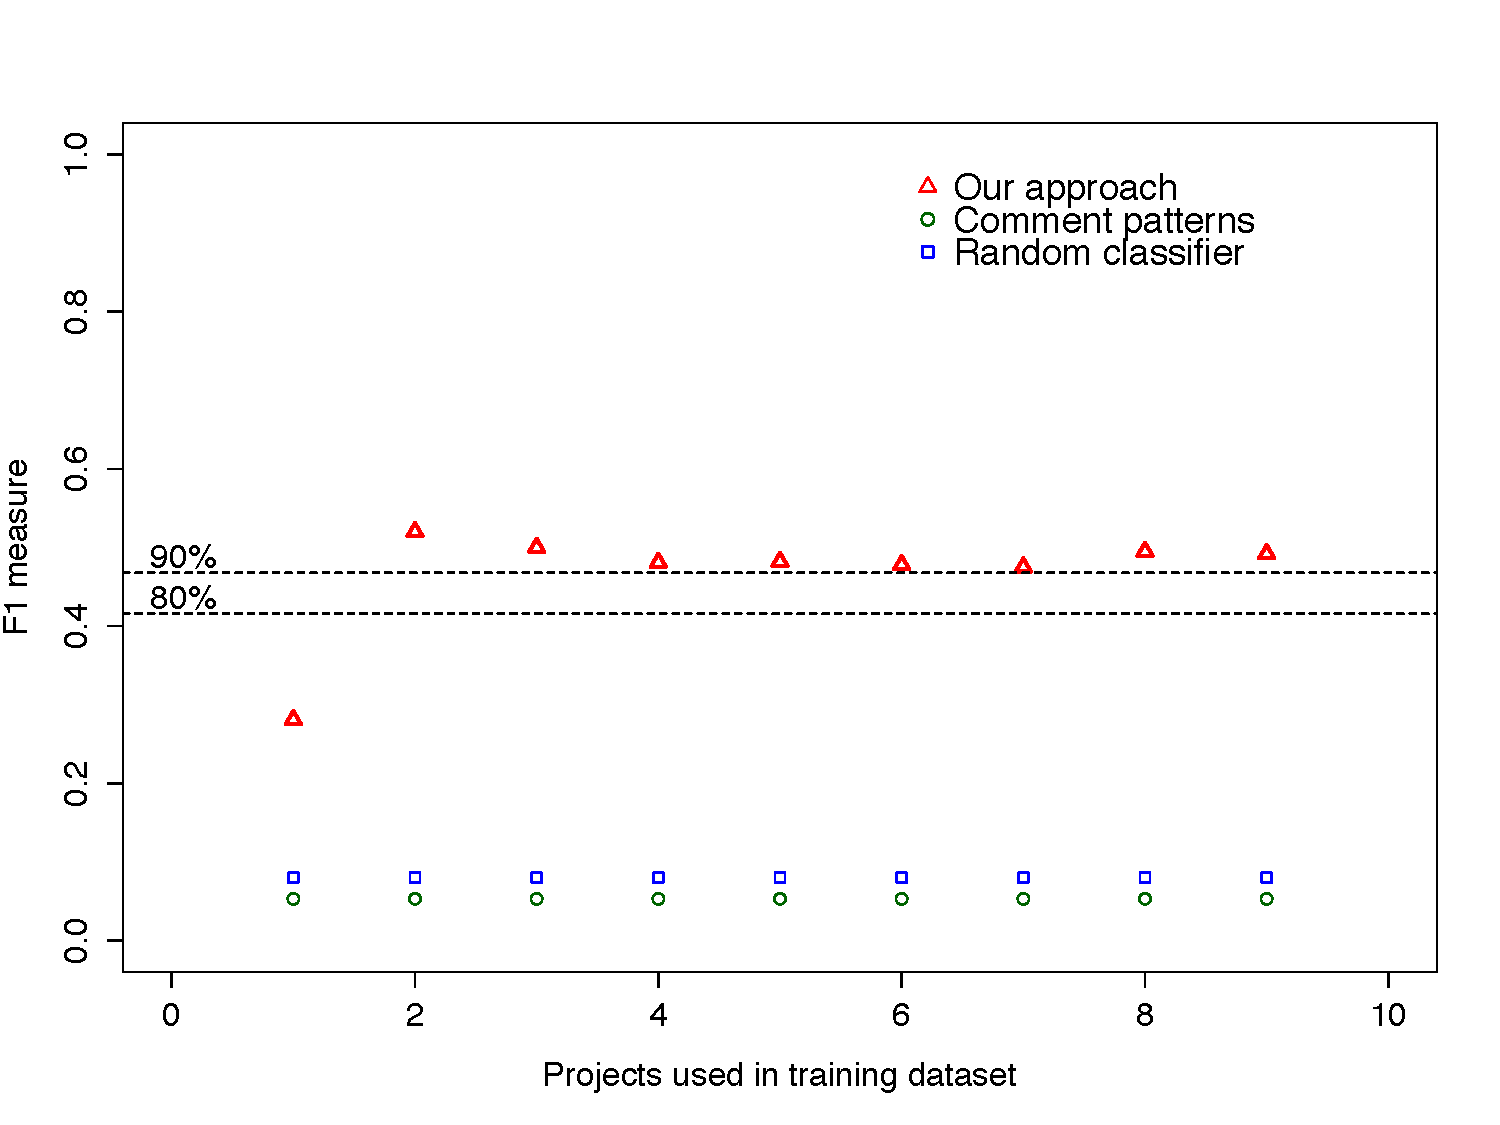
\includegraphics[width=0.49\textwidth]{figures/appendix/iteration_details/design_jfreechart.pdf}
  \vspace{-9mm}
  \caption{JFreeChart Design Debt Classification}
  \label{fig:design_jfreechart}
\end{figure}

\clearpage
\begin{figure}[thb!]
  \centering
  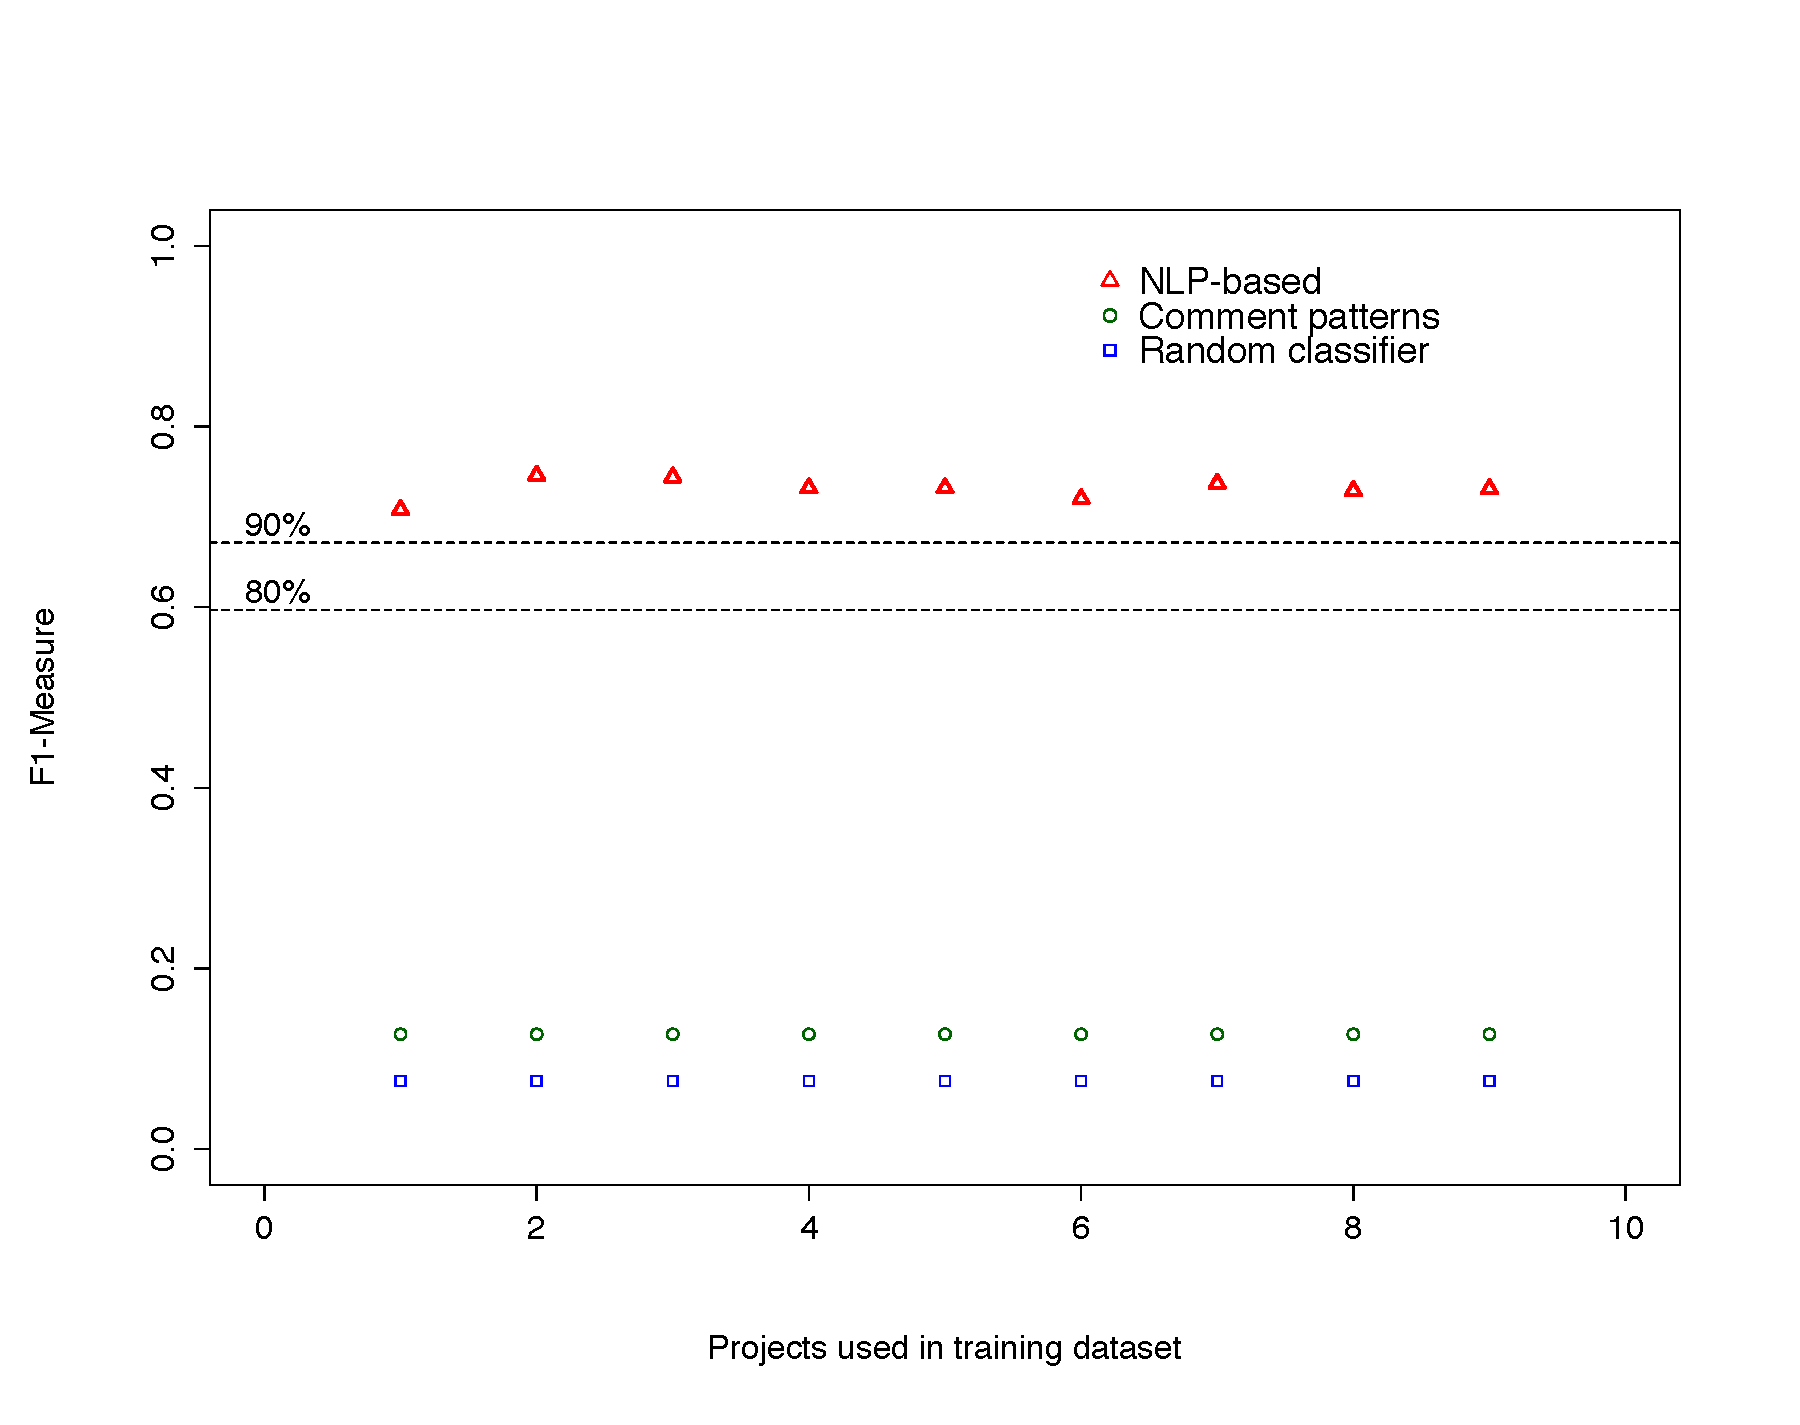
\includegraphics[width=0.49\textwidth]{figures/appendix/iteration_details/design_jmeter.pdf}
  \caption{Jmeter Design Debt Classification}
  \label{fig:design_jmeter}
  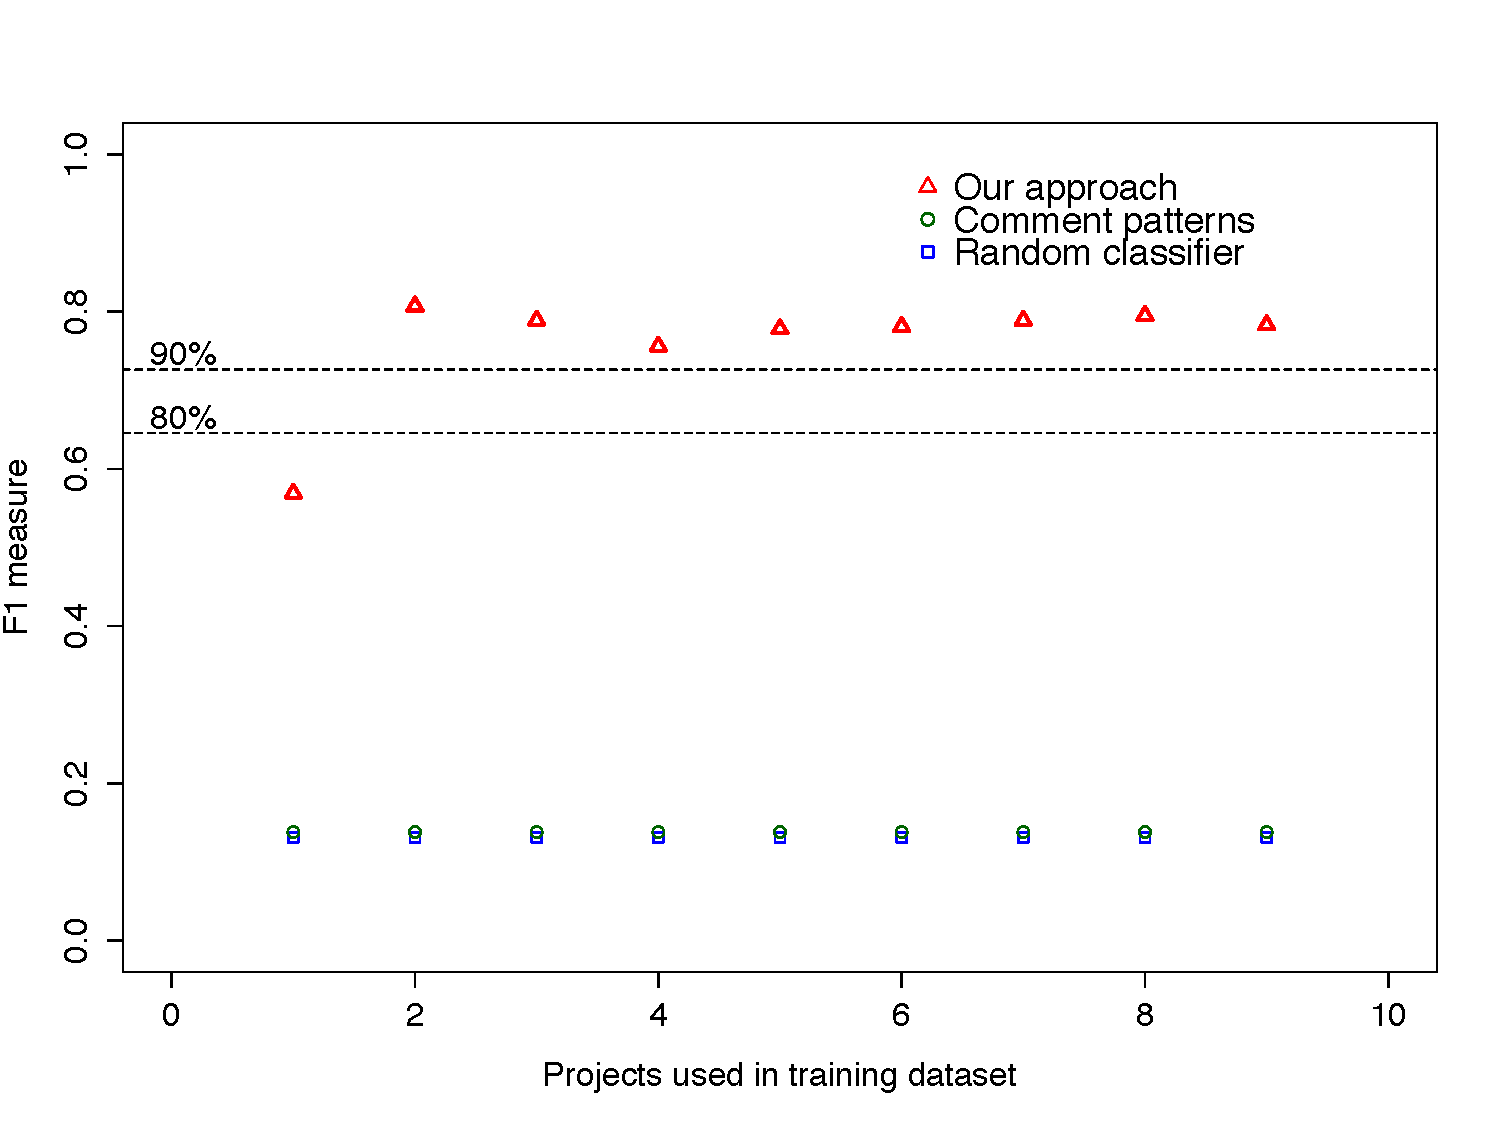
\includegraphics[width=0.49\textwidth]{figures/appendix/iteration_details/design_jruby.pdf}
   \caption{JRuby Design Debt Classification}
   \label{fig:design_jruby}
   \centering
   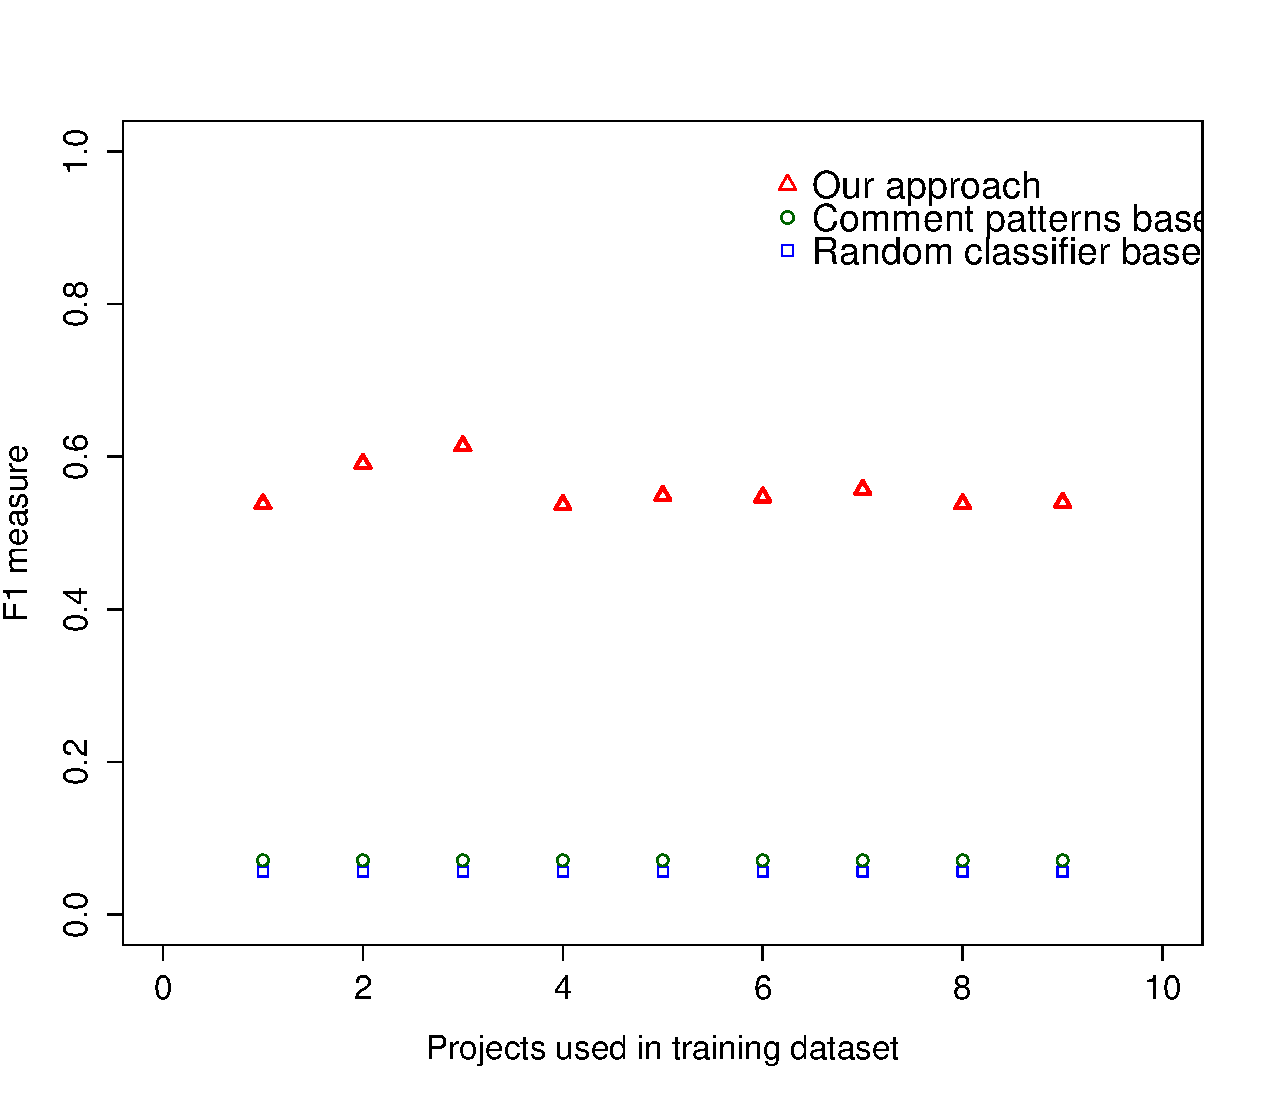
\includegraphics[width=0.49\textwidth]{figures/appendix/iteration_details/design_sql12.pdf}
   \caption{SQuirrel Design Debt Classification}
   \label{fig:design_sql}
\end{figure}
 
\begin{figure}[thb!]    
  \centering
  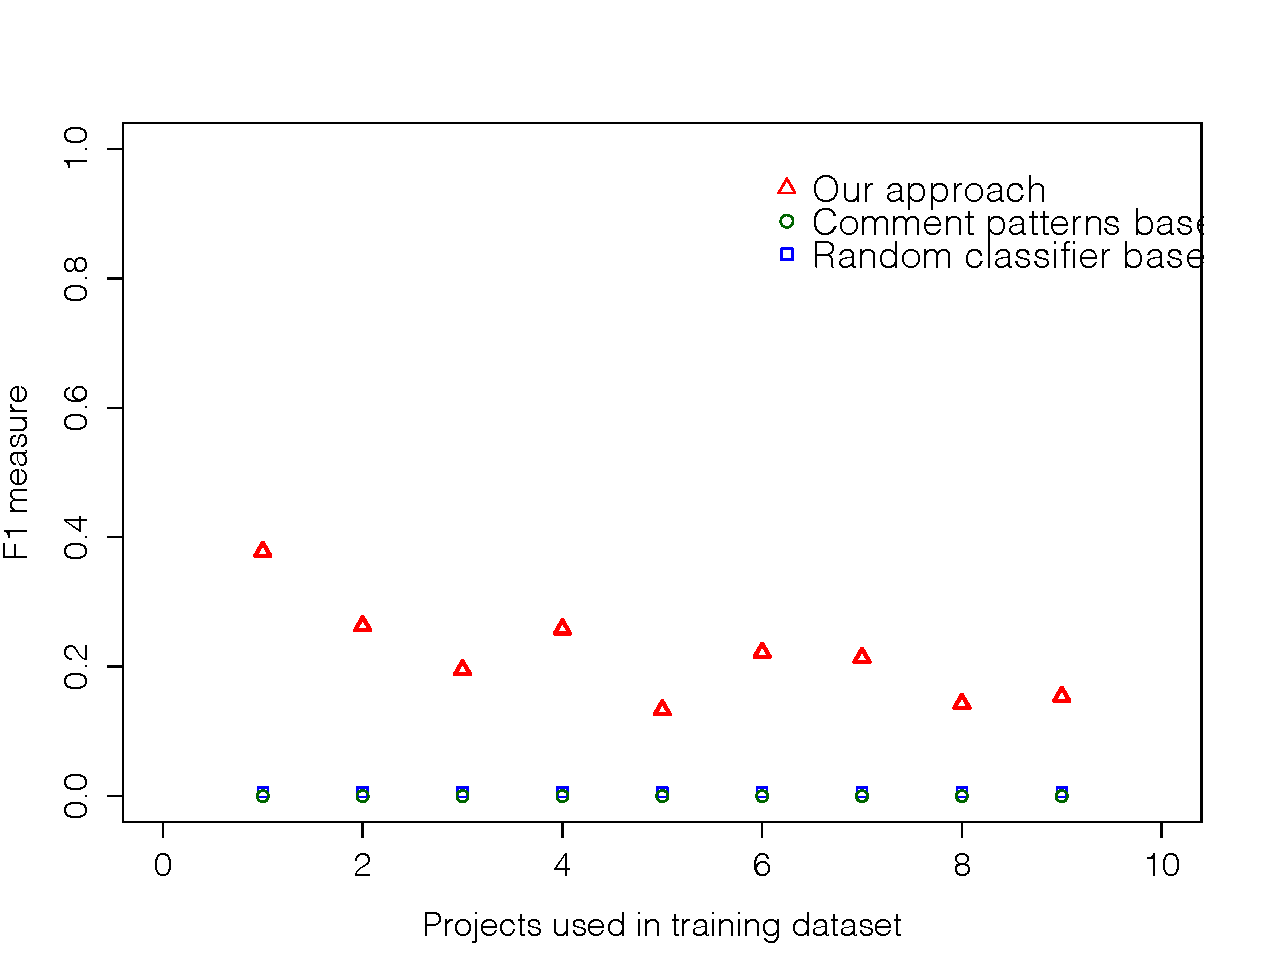
\includegraphics[width=0.49\textwidth]{figures/appendix/iteration_details/implementation_ant.pdf}
  \caption{Ant Requirement Debt Classification}
  \label{fig:implementation_ant}
  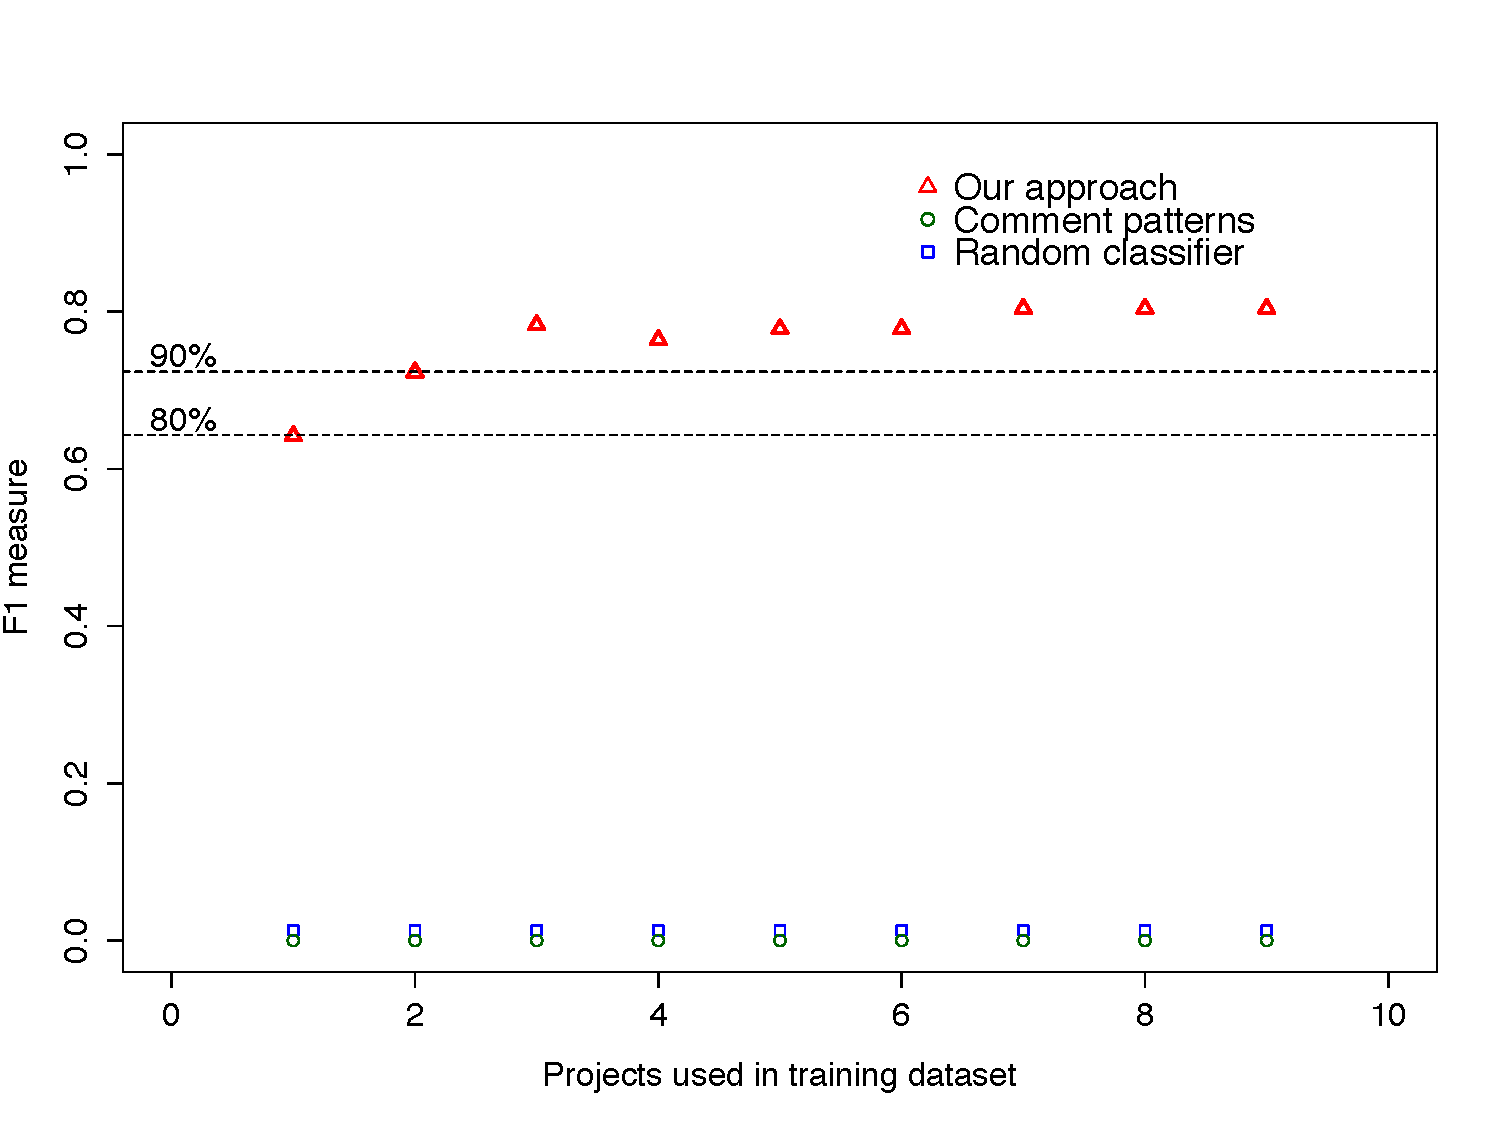
\includegraphics[width=0.49\textwidth]{figures/appendix/iteration_details/implementation_columba.pdf}
  \caption{Columba Requirement Debt Classification}
  \label{fig:implementation_columba}
  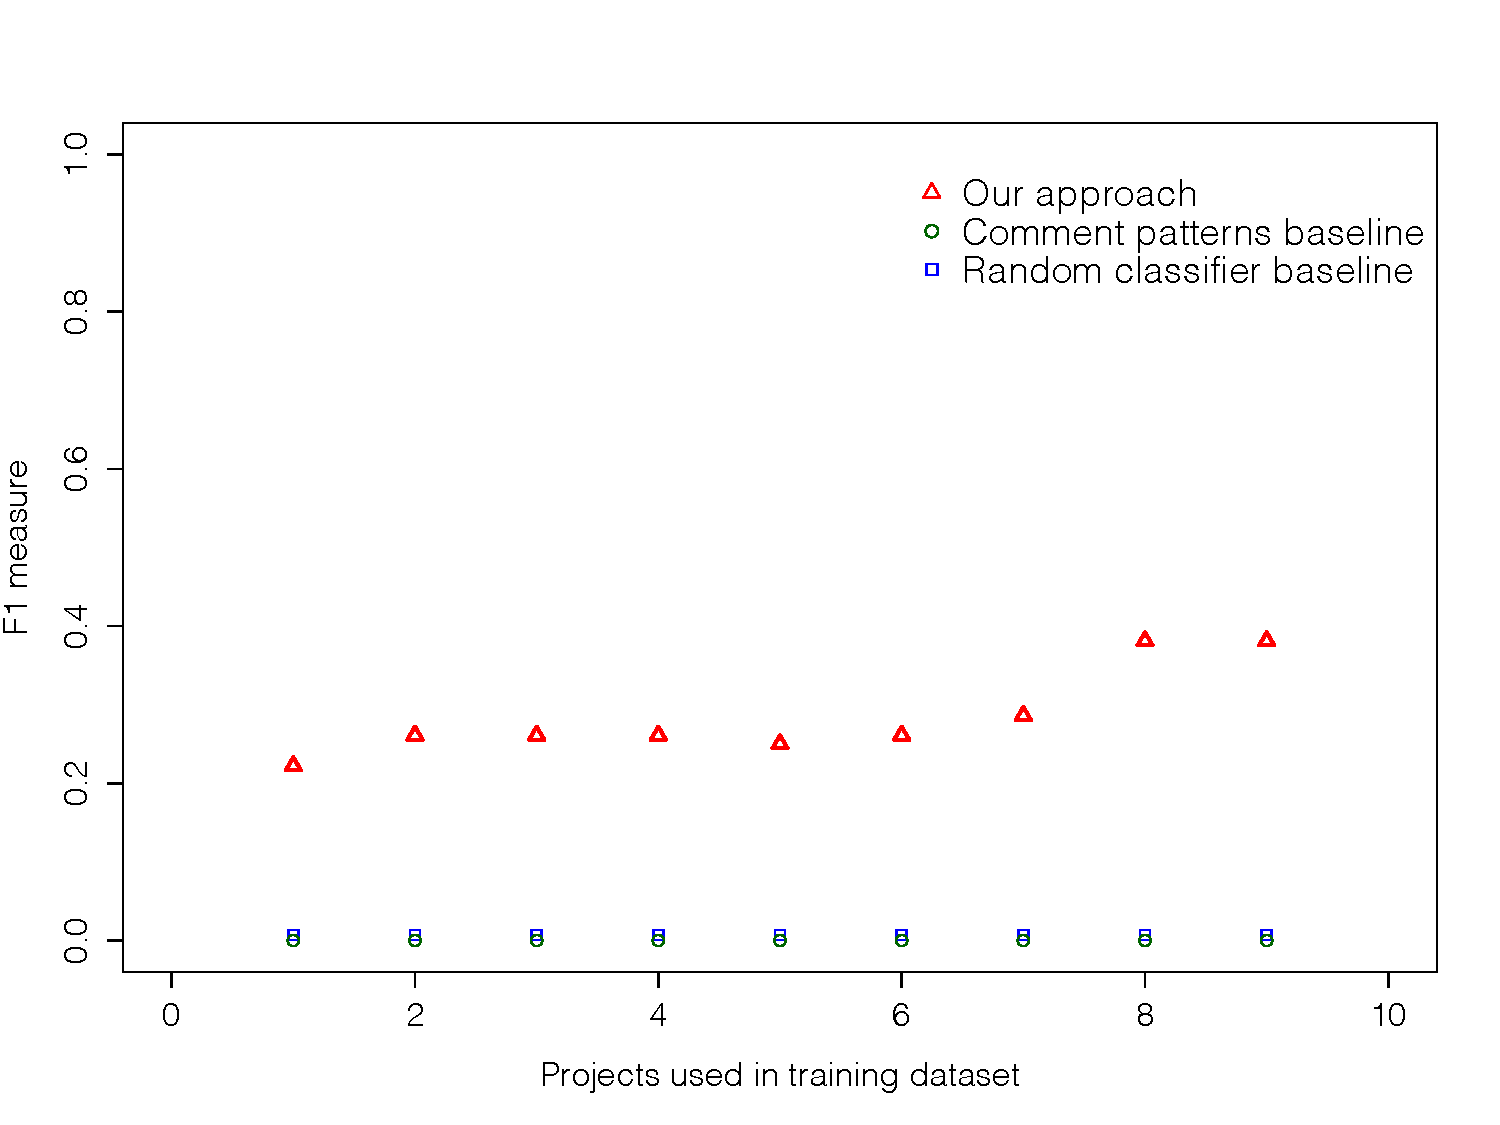
\includegraphics[width=0.49\textwidth]{figures/appendix/iteration_details/implementation_emf.pdf}
  \caption{Emf Requirement Debt Classification}
  \label{fig:implementation_emf}
\end{figure}

\clearpage
\begin{figure}[thb!]
  \centering
  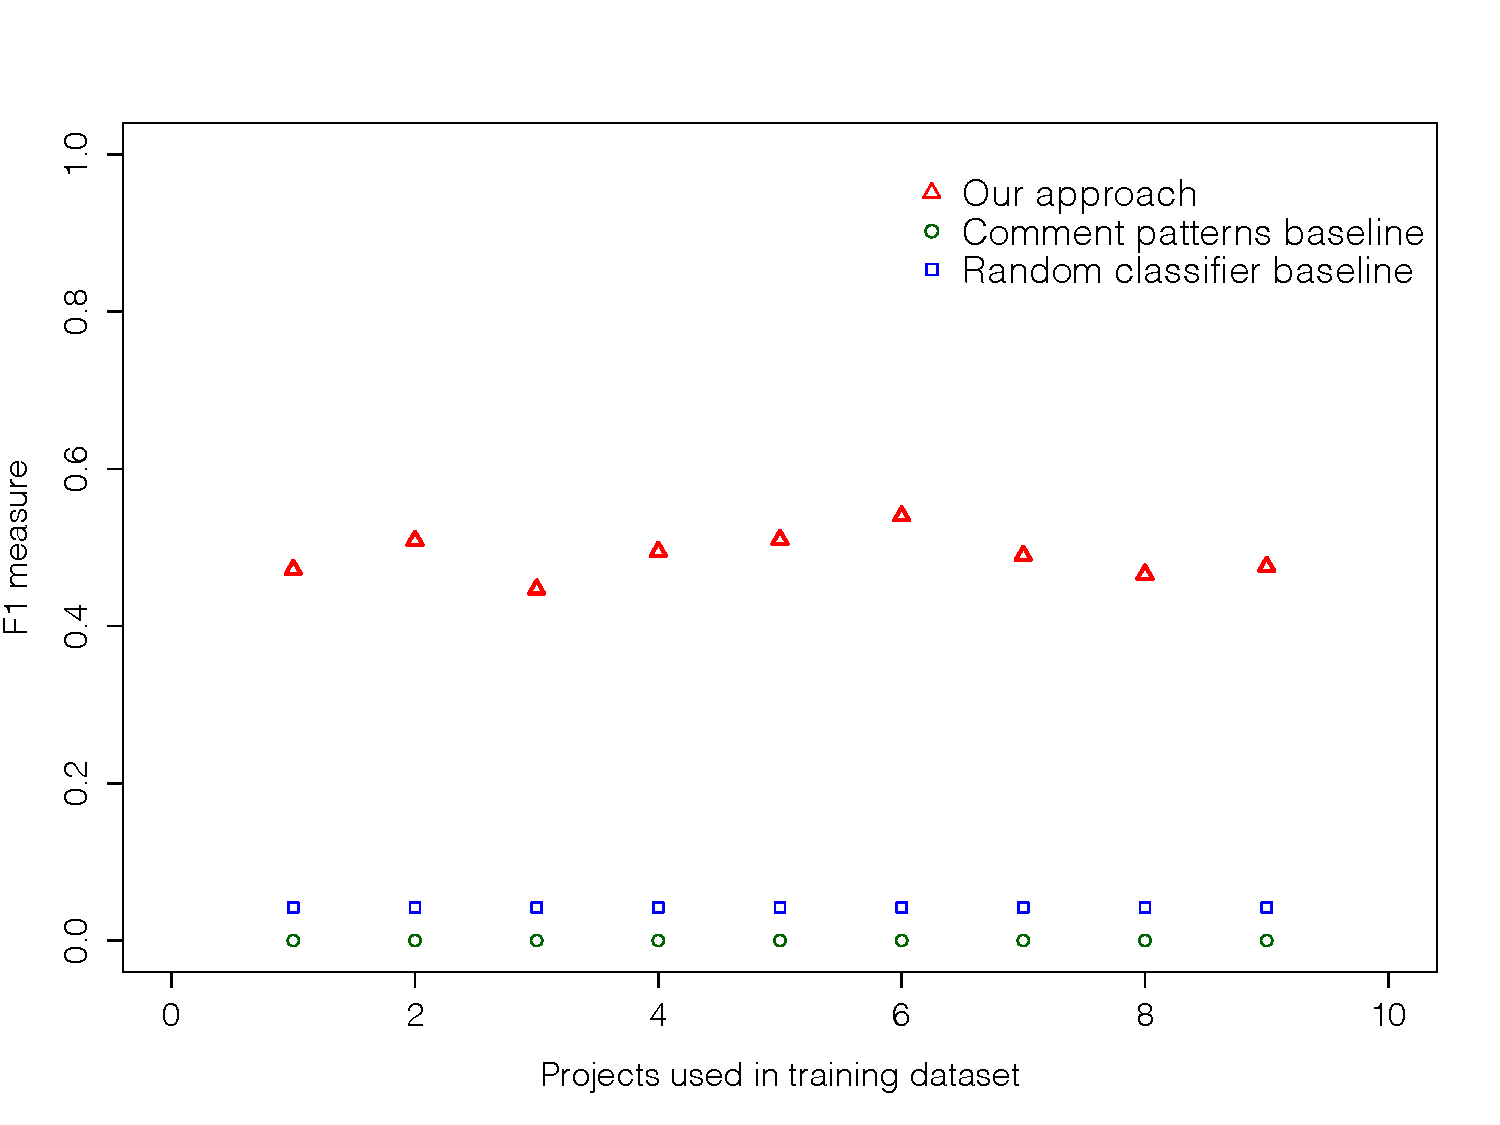
\includegraphics[width=0.49\textwidth]{figures/appendix/iteration_details/implementation_hibernate.pdf}
  \caption{Hibernate Requirement Debt Classification}
  \label{fig:implementation_hibernate}
  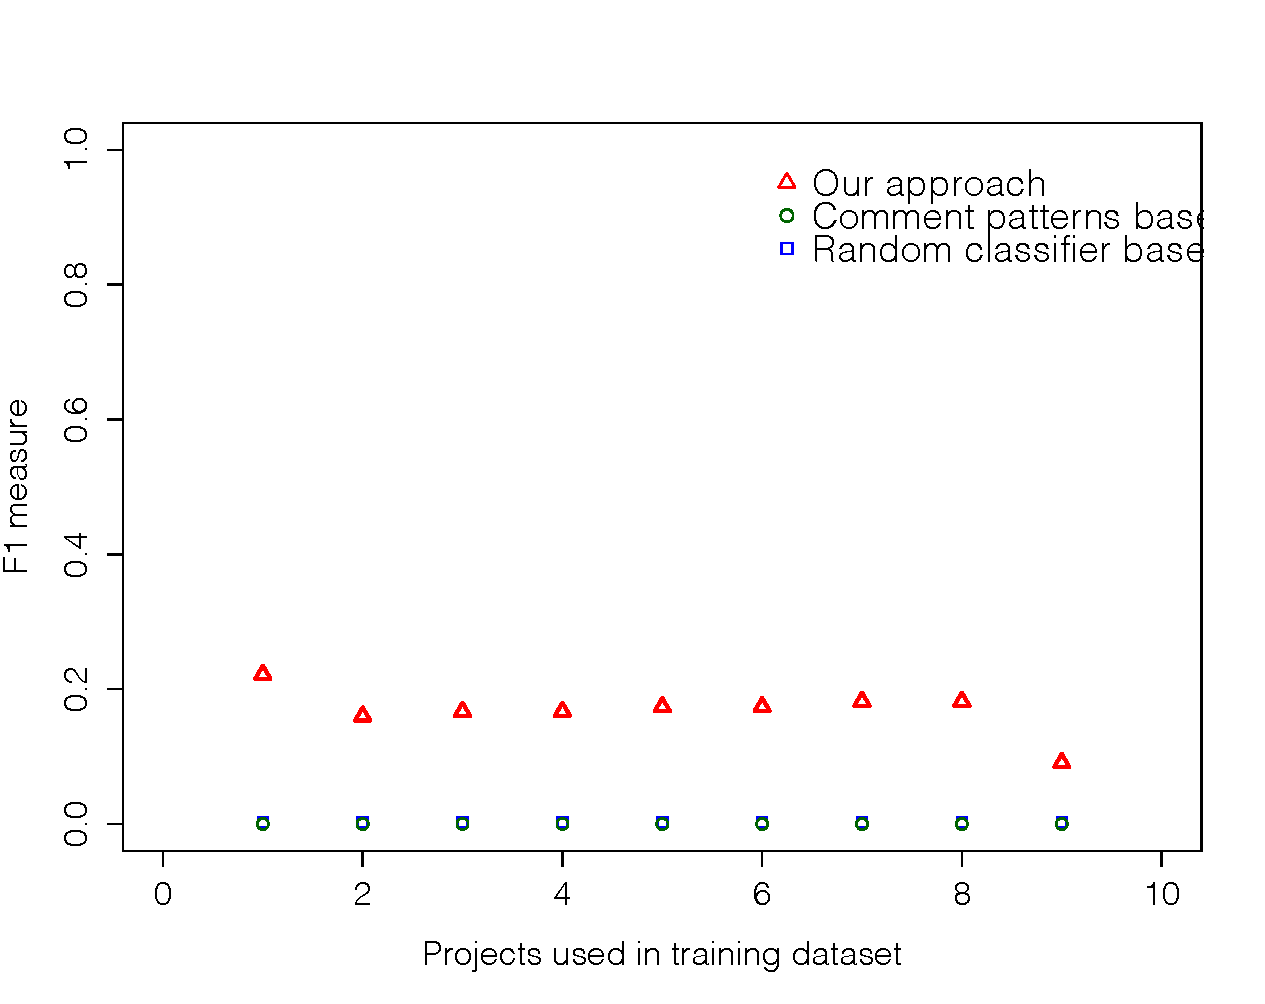
\includegraphics[width=0.49\textwidth]{figures/appendix/iteration_details/implementation_jedit.pdf}
  \caption{JEdit Requirement Debt Classification}
  \label{fig:implementation_jedit}
  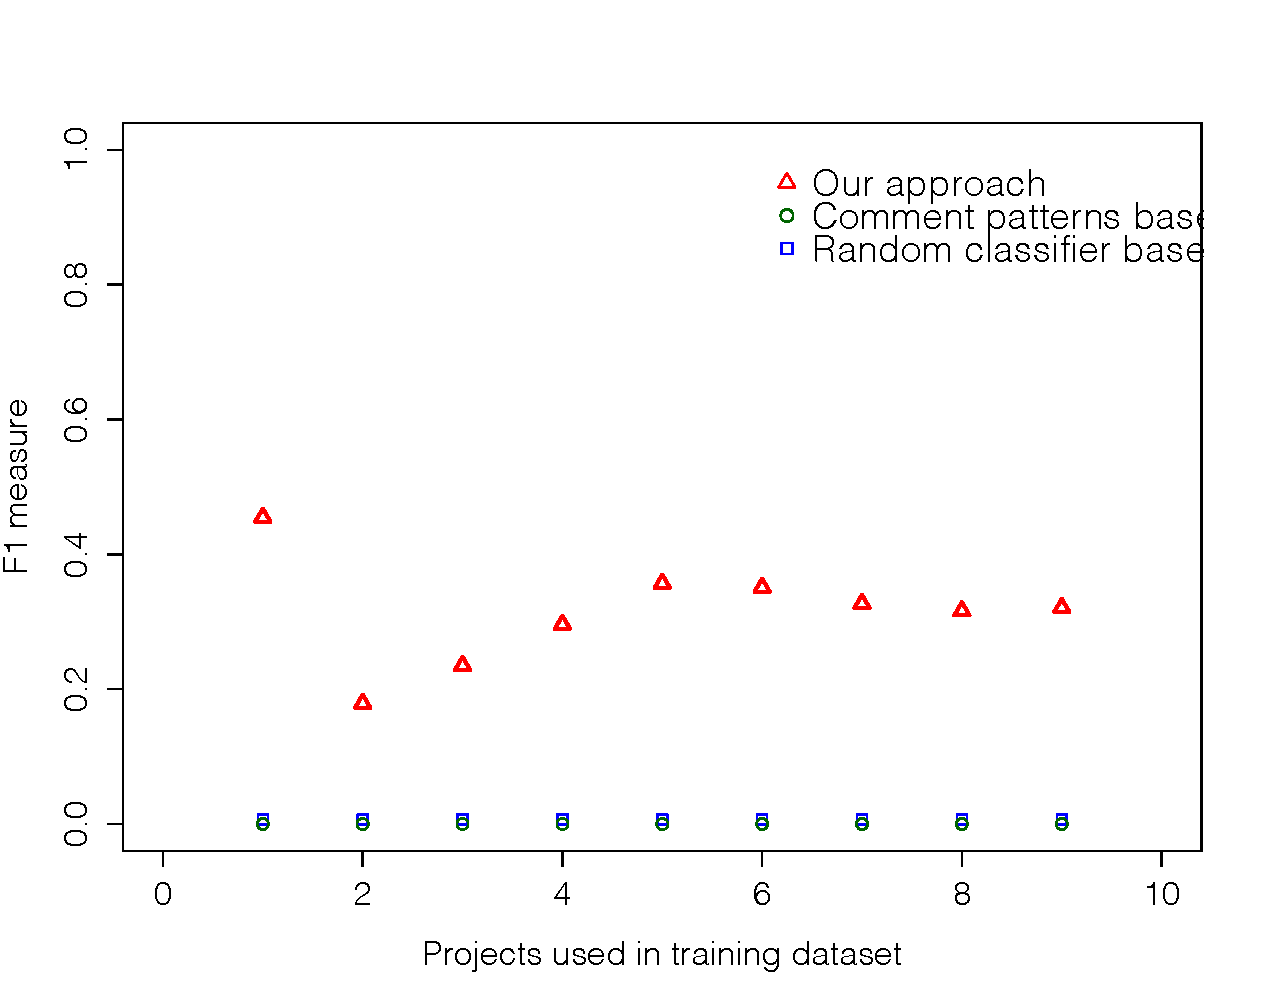
\includegraphics[width=0.49\textwidth]{figures/appendix/iteration_details/implementation_jfreechart.pdf}
  \caption{JFreeChart Requirement Debt Classification}
  \label{fig:implementation_jfreechart}  
    
\end{figure}

\begin{figure}[thb!]
  \centering
  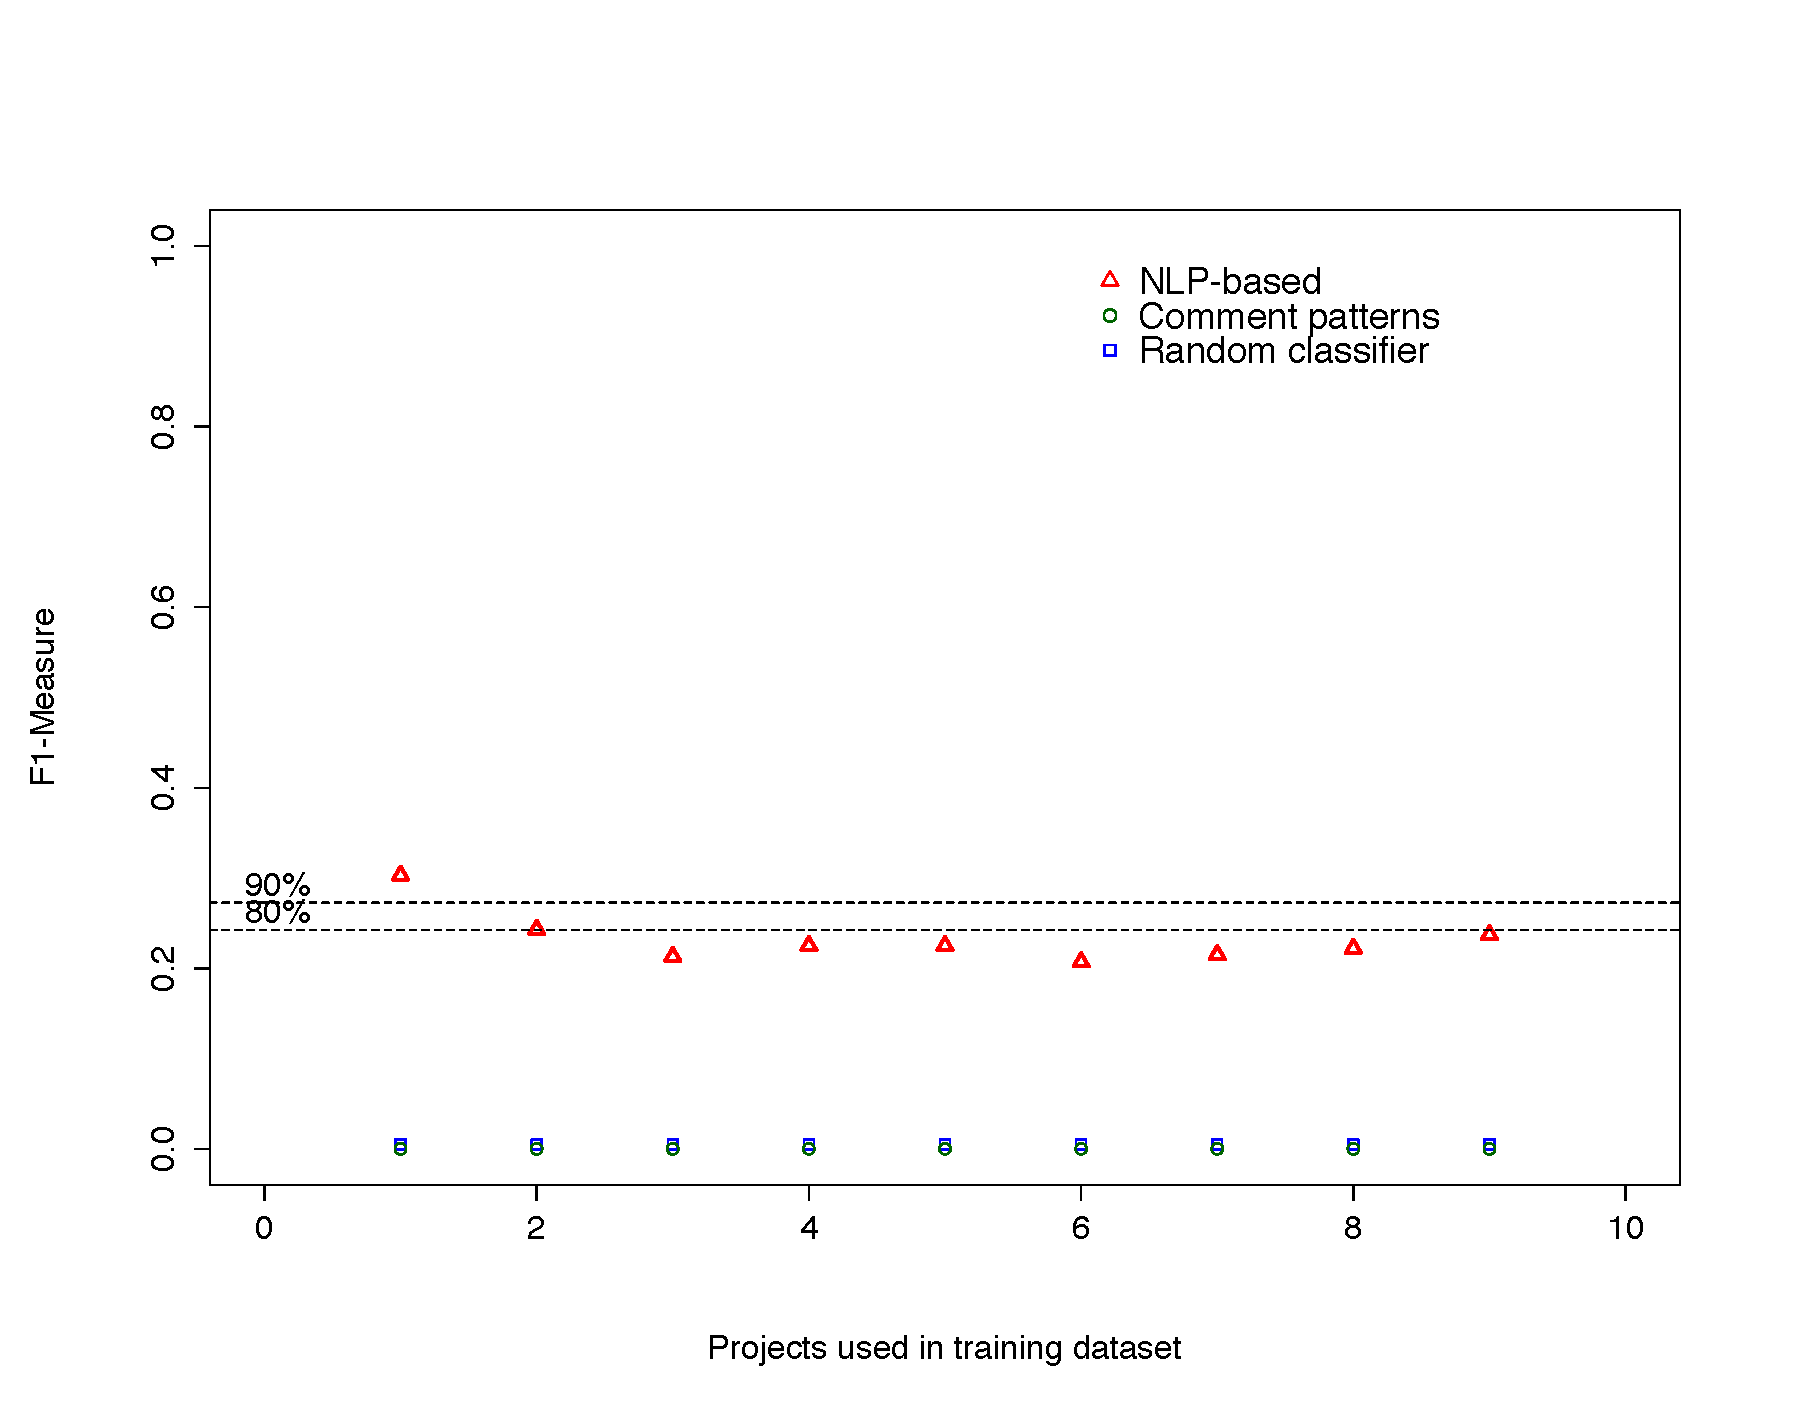
\includegraphics[width=0.49\textwidth]{figures/appendix/iteration_details/implementation_jmeter.pdf}
  \caption{Jmeter Requirement Debt Classification}
  \label{fig:implementation_jmeter}
  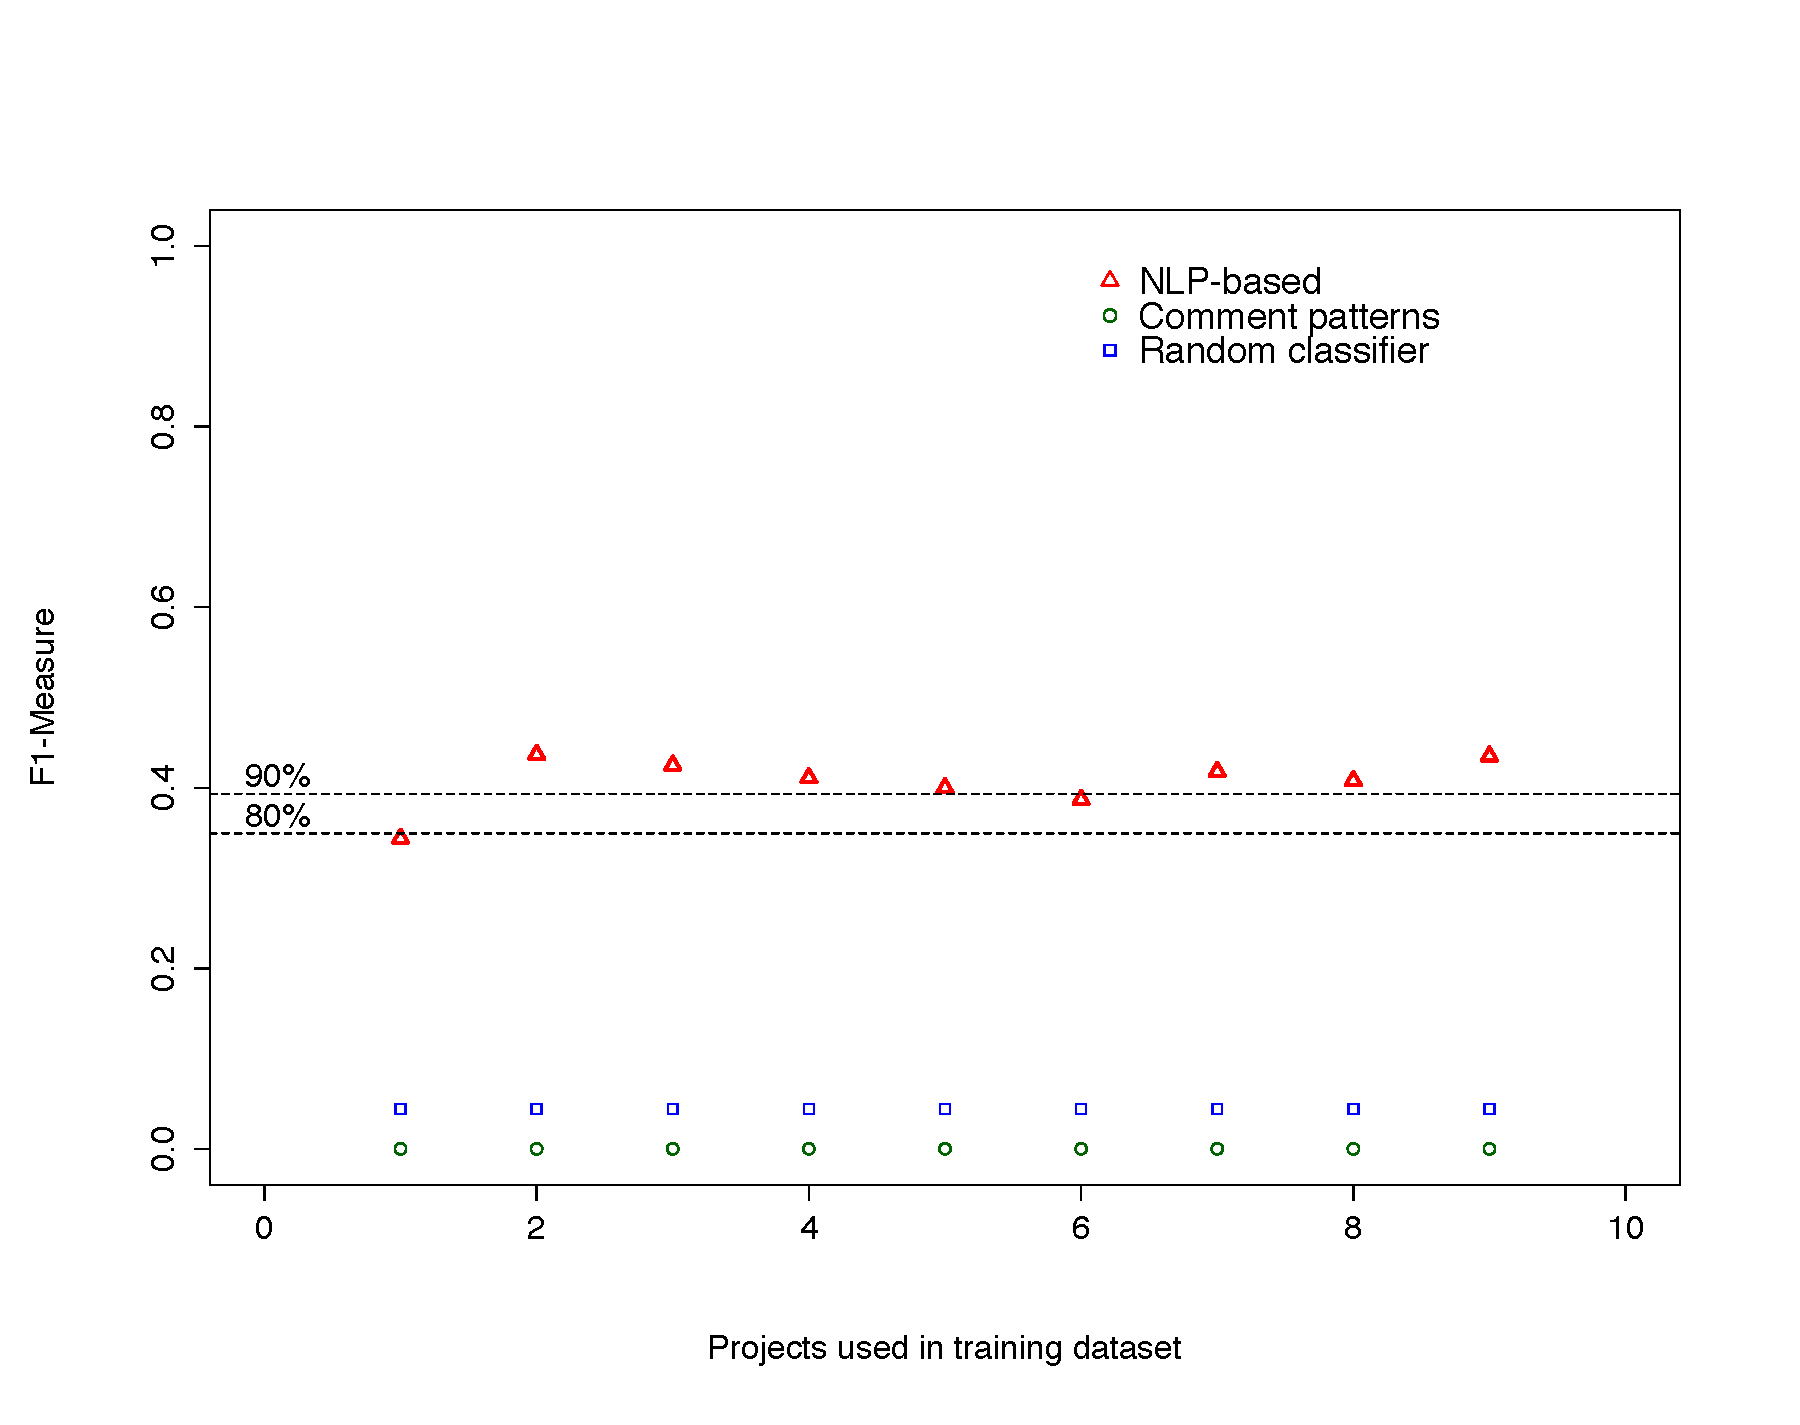
\includegraphics[width=0.49\textwidth]{figures/appendix/iteration_details/implementation_jruby.pdf}
  \caption{JRuby Requirement Debt Classification}
  \label{fig:implementation_jruby}
  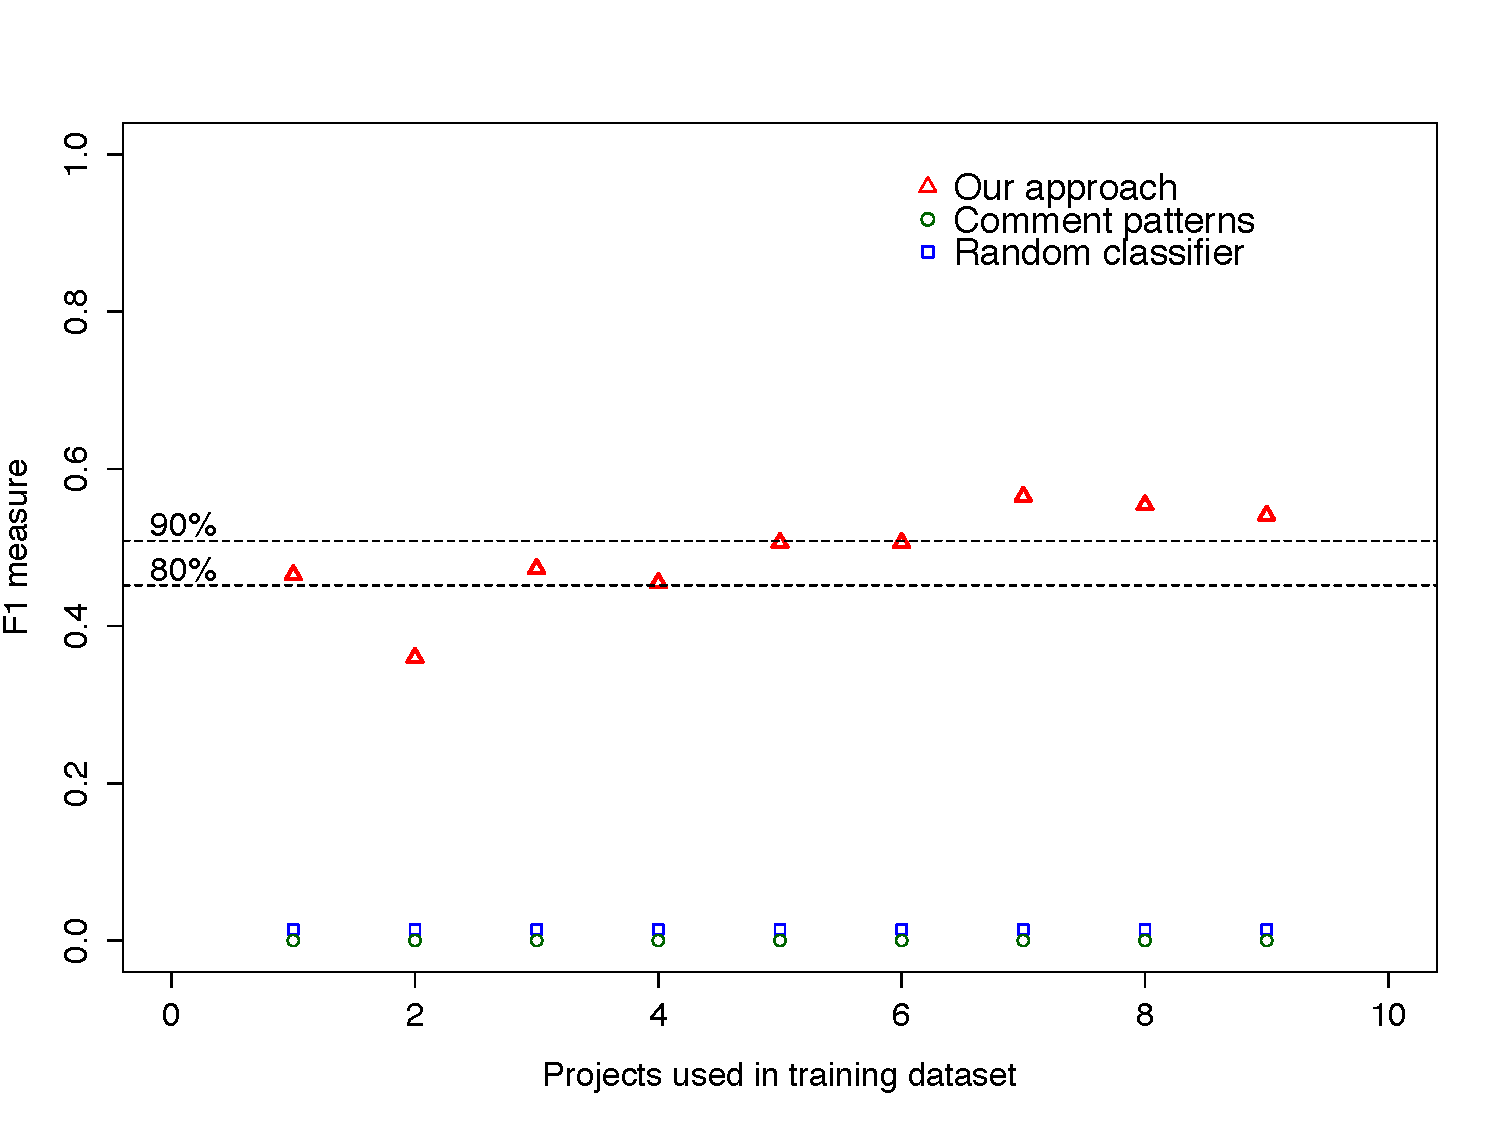
\includegraphics[width=0.49\textwidth]{figures/appendix/iteration_details/implementation_sql12.pdf}
  \caption{SQuirrel Requirement Debt Classification}
  \label{fig:implementation_sql}    
\end{figure}


% \begin{table}[!hbt]
%     \begin{center}
%         \caption{Effects in the F1 measure of the Design training datasets}
%         \label{tbl:detailed_comparison_design_training_dataset}
%         \begin{tabular}{l| c c c}
%         \toprule
%         \thead{Project} & \thead{Anagrams\\Dataset} & \thead{Capitalized\\Dataset} & \thead{Lowercase\\Dataset}\\
%         \midrule
%         Apache Ant    &  0.511   & 0.471 &  0.517    \\
%         Apache Jmeter &  0.744   & 0.704 &  0.731    \\
%         ArgoUML       &  0.801   & 0.819 &  0.814    \\
%         Columba       &  0.815   & 0.586 &  0.601    \\
%         EMF           &  0.532   & 0.397 &  0.470    \\
%         Hibernate     &  0.742   & 0.692 &  0.744    \\
%         JEdit         &  0.493   & 0.465 &  0.509    \\
%         JFreeChart    &  0.452   & 0.503 &  0.492    \\
%         JRuby         &  0.817   & 0.795 &  0.783    \\
%         SQuirrel      &  0.587   & 0.543 &  0.540    \\
%         \bottomrule
%         \end{tabular}
%     \end{center}    
% \end{table}

% \clearpage

% \begin{figure}[thb!]
%   \centering
%   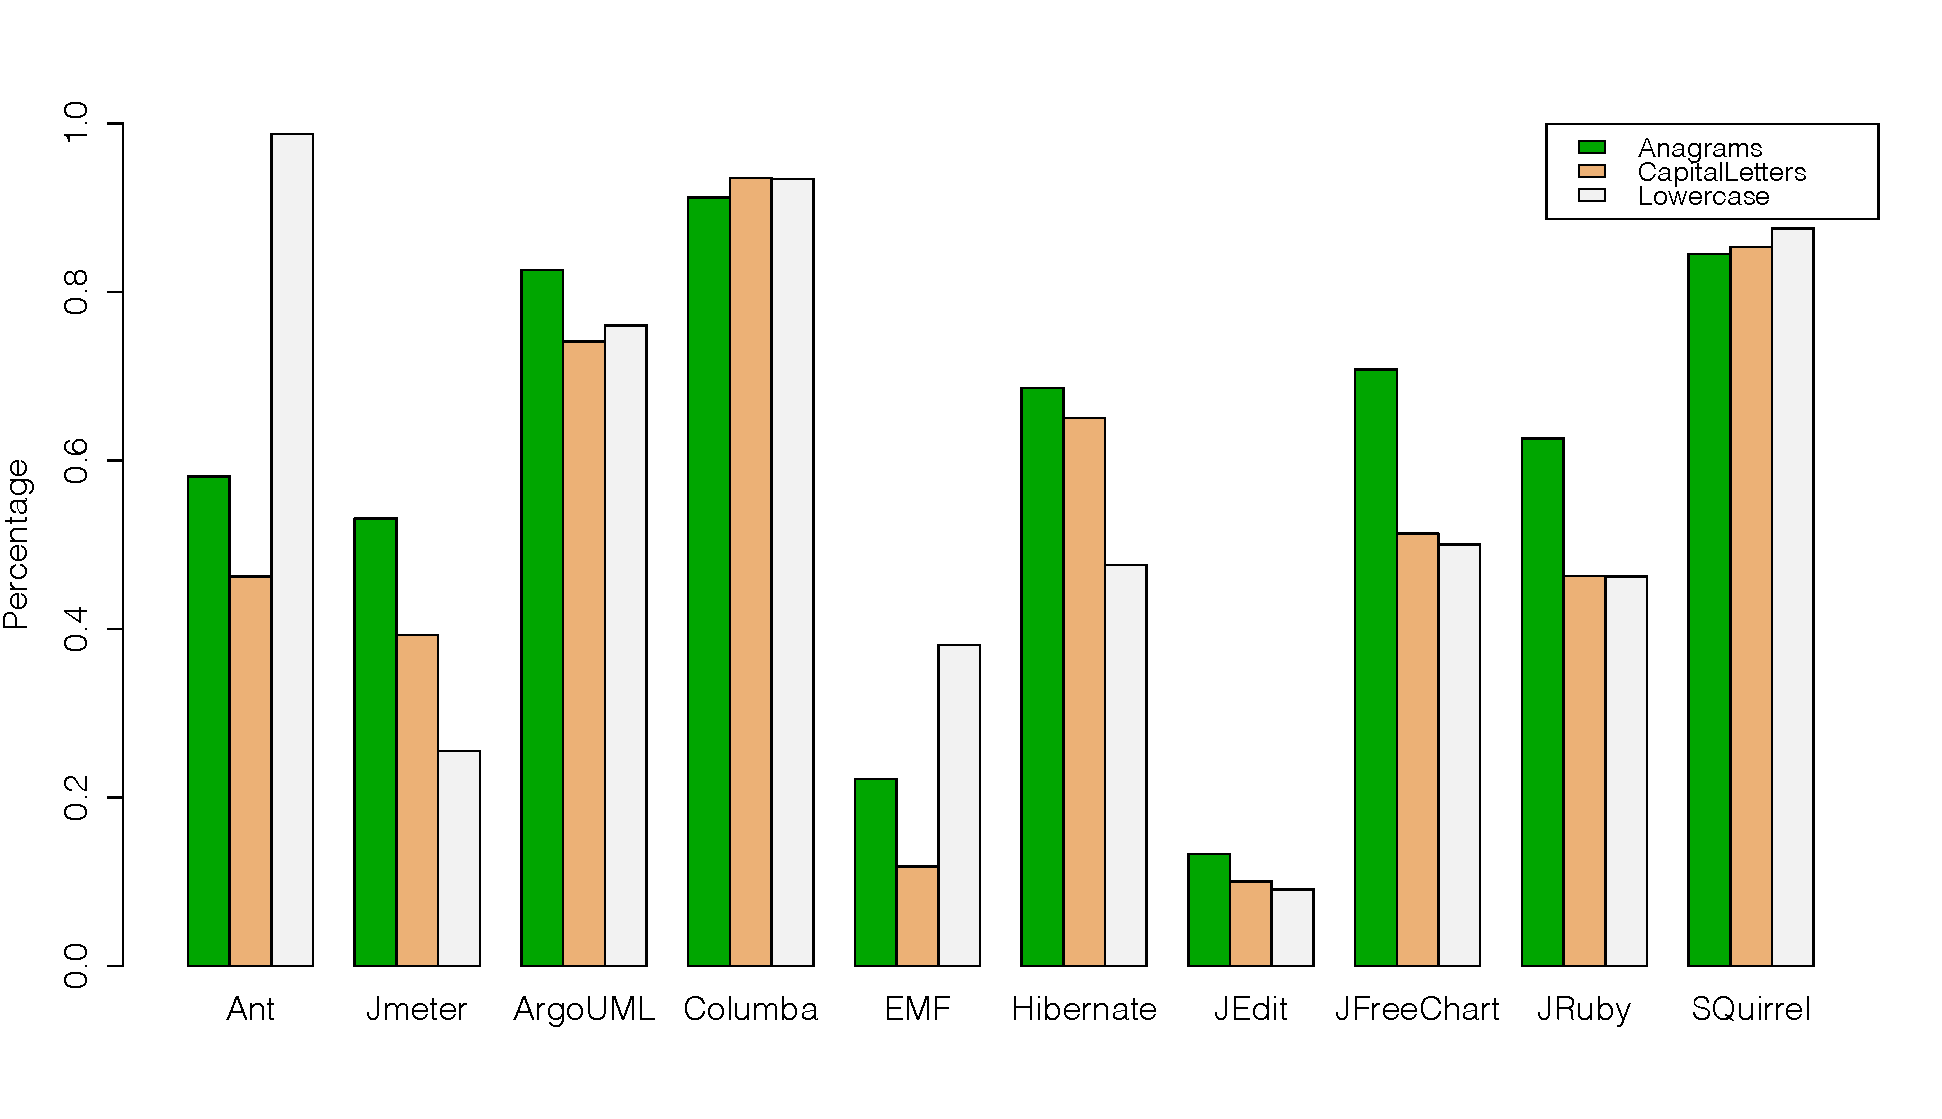
\includegraphics[width=0.50\textwidth]{figures/appendix/detailed_comparison_requirement_training_dataset.pdf}
%   \vspace{-3mm}
%   \caption{Detailed comparison of the changes in the requirements training datasets}
%   \label{fig:detailed_comparison_requirement_training_dataset}
% \end{figure}

% \begin{figure}[thb!]
%   \centering
%   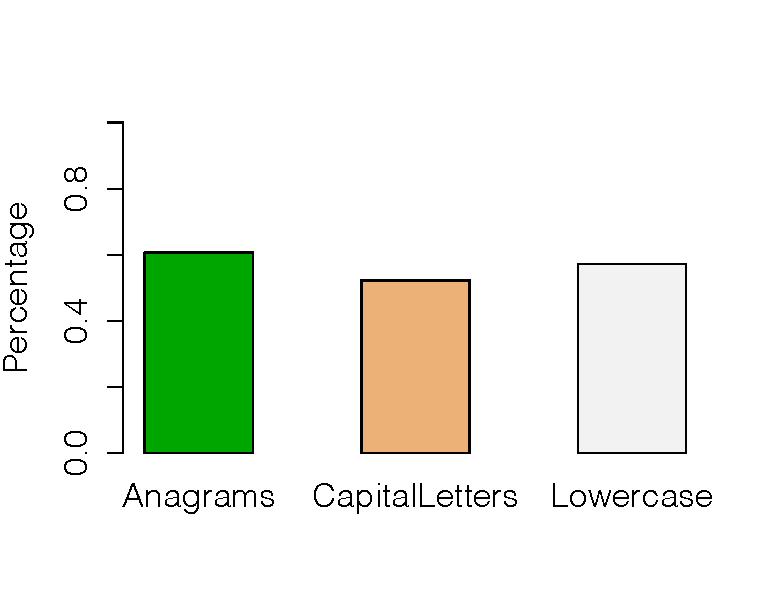
\includegraphics[width=0.50\textwidth]{figures/appendix/average_comparison_requeriment_training_dataset.pdf}
%   \vspace{-3mm}
%   \caption{Average comparison of the changes in the requirements training datasets}
%   \label{fig:average_comparison_requirement_training_dataset}
% \end{figure}

% \begin{table}[!hbt]
%     \begin{center}
%         \caption{Effects in the F1 measure of the Requirements training datasets}
%         \label{tbl:detailed_comparison_requirement_training_dataset}
%         \begin{tabular}{l| c c c}
%         \toprule
%         \thead{Project} & \thead{Anagrams\\Dataset} & \thead{Capitalized\\Dataset} & \thead{Lowercase\\Dataset}\\
%         \midrule
%         Apache Ant    &  0.581 & 0.462 & 0.987  \\
%         Apache Jmeter &  0.531 & 0.393 & 0.255  \\
%         ArgoUML       &  0.826 & 0.741 & 0.760  \\
%         Columba       &  0.912 & 0.935 & 0.934  \\
%         EMF           &  0.222 & 0.118 & 0.381  \\
%         Hibernate     &  0.686 & 0.650 & 0.476  \\
%         JEdit         &  0.133 & 0.100 & 0.091  \\
%         JFreeChart    &  0.708 & 0.513 & 0.500  \\
%         JRuby         &  0.626 & 0.463 & 0.462  \\
%         SQuirrel      &  0.845 & 0.853 & 0.875  \\
%         \bottomrule
%         \end{tabular}
%     \end{center}    
% \end{table}


\clearpage
\subsection*{Detailed Precision and Recall Values When Different Underlying Classifiers are Used}

When presenting the results in Section~\ref{sec:underlying_classifier}, we only presented the F1-measures. Here, we present the detailed precision and recall values that make up the F1-measures presented earlier.

\begin{table}[h]
  \begin{minipage}{\textwidth}
    \begin{center}
        \caption{Comparison Between Different Classifiers Algorithms for Design Debt}
        \label{tbl:improvement_f1measure_between_classifiers_design}
        \begin{tabular}{l| c c c|| c c c|| c c c }
        \toprule

        \multirow{4}{*}{\textbf{\thead{Project}}} & \multicolumn{3}{c||}{\textbf{\thead{Logistic Regression}}} & \multicolumn{3}{c||}{\textbf{\thead{Naive Bayes}}} & \multicolumn{3}{c}{\textbf{\thead{Binary}}} 
        
        \\ 
        \cmidrule{2-10}
        
        & \textbf{\thead{Precision}} & \textbf{\thead{Recall}} & \textbf{\thead{F1 measure}} & \textbf{\thead{Precision}} & \textbf{\thead{Recall}} & \textbf{\thead{F1 measure}} & \textbf{\thead{Precision}} & \textbf{\thead{Recall}} & \textbf{\thead{F1 measure}}\\
        \midrule                                                  
        \textbf{Ant}          &  0.554 & 0.484 &  0.517 &  0.072 & 0.874 & 0.134 &  0.620 & 0.516 & 0.563  \\
        \textbf{ArgoUML}      &  0.788 & 0.843 &  0.814 &  0.358 & 0.985 & 0.525 &  0.790 & 0.858 & 0.822  \\
        \textbf{Columba}      &  0.792 & 0.484 &  0.601 &  0.181 & 0.786 & 0.294 &  0.840 & 0.500 & 0.627  \\
        \textbf{EMF}          &  0.574 & 0.397 &  0.470 &  0.057 & 0.872 & 0.106 &  0.633 & 0.397 & 0.488  \\
        \textbf{Hibernate}    &  0.877 & 0.645 &  0.744 &  0.288 & 0.890 & 0.435 &  0.895 & 0.670 & 0.767  \\
        \textbf{JEdit}        &  0.779 & 0.378 &  0.509 &  0.227 & 0.791 & 0.353 &  0.807 & 0.342 & 0.480  \\
        \textbf{JFreeChart}   &  0.646 & 0.397 &  0.492 &  0.140 & 0.560 & 0.224 &  0.658 & 0.397 & 0.495  \\
        \textbf{Jmeter}       &  0.808 & 0.668 &  0.731 &  0.224 & 0.801 & 0.350 &  0.819 & 0.671 & 0.737  \\
        \textbf{JRuby}        &  0.798 & 0.770 &  0.783 &  0.275 & 0.971 & 0.429 &  0.815 & 0.808 & 0.811  \\
        \textbf{SQuirrel}     &  0.544 & 0.536 &  0.540 &  0.133 & 0.947 & 0.233 &  0.567 & 0.550 & 0.558  \\
        \midrule                                                  
        \textbf{Average}      &  0.716 &   0.5602 &  0.6201 &  0.1955  & 0.8477  & 0.3083 & 0.7444  & 0.5709 & 0.6348  \\
        \bottomrule
        \end{tabular}
    \end{center}
  \end{minipage}    
\end{table}

\begin{table}[h]
  \begin{minipage}{\textwidth}
    \begin{center}
        \caption{Comparison Between Different Classifiers Algorithms for Requirement Debt}
        \label{tbl:improvement_f1measure_between_classifiers_requirement}
        \begin{tabular}{l| c c c|| c c c|| c c c }
        \toprule
        \multirow{4}{*}{\textbf{\thead{Project}}} & \multicolumn{3}{c||}{\textbf{\thead{Logistic Regression}}} & \multicolumn{3}{c||}{\textbf{\thead{Naive Bayes}}} & \multicolumn{3}{c}{\textbf{\thead{Binary}}} 
        
        \\ 
        \cmidrule{2-10}
        
        & \textbf{\thead{Precision}} & \textbf{\thead{Recall}} & \textbf{\thead{F1 measure}} & \textbf{\thead{Precision}} & \textbf{\thead{Recall}} & \textbf{\thead{F1 measure}} & \textbf{\thead{Precision}} & \textbf{\thead{Recall}} & \textbf{\thead{F1 measure}}\\
        \midrule                                                  
        \textbf{Ant}          &  0.154 & 0.154 & 0.154 & 0.007 &  0.769 & 0.013 & 0.188 & 0.231 & 0.207 \\
        \textbf{ArgoUML}      &  0.663 & 0.540 & 0.595 & 0.119 &  0.808 & 0.207 & 0.659 & 0.569 & 0.611 \\
        \textbf{Columba}      &  0.755 & 0.860 & 0.804 & 0.030 &  0.930 & 0.057 & 0.755 & 0.860 & 0.804 \\
        \textbf{EMF}          &  0.800 & 0.250 & 0.381 & 0.009 &  1.000 & 0.018 & 0.800 & 0.250 & 0.381 \\
        \textbf{Hibernate}    &  0.610 & 0.391 & 0.476 & 0.041 &  0.781 & 0.078 & 0.615 & 0.375 & 0.466 \\
        \textbf{JEdit}        &  0.125 & 0.071 & 0.091 & 0.011 &  0.857 & 0.022 & 0.143 & 0.071 & 0.095 \\
        \textbf{JFreeChart}   &  0.220 & 0.600 & 0.321 & 0.009 &  0.800 & 0.018 & 0.179 & 0.467 & 0.259 \\
        \textbf{Jmeter}       &  0.153 & 0.524 & 0.237 & 0.011 &  0.952 & 0.022 & 0.180 & 0.524 & 0.268 \\
        \textbf{JRuby}        &  0.686 & 0.318 & 0.435 & 0.058 &  0.836 & 0.109 & 0.679 & 0.327 & 0.442 \\
        \textbf{SQuirrel}     &  0.657 & 0.460 & 0.541 & 0.018 &  0.900 & 0.036 & 0.455 & 0.500 & 0.476 \\
        \midrule                                                  
        \textbf{Average}      & 0.4823 &  0.4168 & 0.4035 & 0.0313 & 0.8633 & 0.058  & 0.4653 & 0.4174 & 0.4009 \\
        \bottomrule
        \end{tabular}
    \end{center}
  \end{minipage}    
\end{table} 

% \clearpage

% \begin{table}[h]
%   \begin{minipage}{\textwidth}
%     \begin{center}
%         \caption{Intersection Between Static Analysis Tools and Self-admitted Technical Debt Using Code Smell Detector) }
%         \label{tbl:intersection_between_static_analysis_tools_and_self_admitted_technical_debt_code_smell_detector}
%         \begin{tabular}{l| c c c c}
%         \toprule
%         \thead{Project} & \thead{\# of files} & \thead{\# of files with \\bad smell} & \thead{\# of files with \\ SATD}  & \thead{\# of files in common}\\
%         \midrule
%         % without Feature Envy and Lazy Class
%         Apache Ant     & 1,475 & 365 & 68  & 46    \\
%         Apache Jmeter  & 1,181 & 395 & 191 & 113   \\
%         ArgoUML        & 2,610 & 708 & 328 & 191   \\
%         Columba        & 1,711 & 396 & 90  & 44    \\
%         EMF            & 1,458 & 558 & 46  & 36    \\
%         Hibernate      & 1,356 & 493 & 182 & 122   \\
%         JEdit          & 800   & 320 & 104 & 78    \\
%         JFreeChart     & 1,065 & 410 & 97  & 69    \\
%         JRuby          & 1,486 & 787 & 141 & 113   \\
%         SQuirrel       & 3,108 & 609 & 131 & 82    \\

%         \bottomrule
%         \end{tabular}
%     \end{center}
%   \end{minipage}    
% \end{table} 

\begin{table}[h]
  \begin{minipage}{\textwidth}
    \begin{center}
        \caption{Intersection Between Static Analysis Tools and Self-admitted Technical Debt Using JDeodorant }
        \label{tbl:intersection_between_static_analysis_tools_and_self_admitted_technical_debt_jdeodorant }
        \begin{tabular}{l| c c c c c c c c c c}
        \toprule
        \thead{Project} & \thead{\# of files} & \thead{\# of \\files with \\ bad \\smell} & \thead{\# of \\files with \\ long \\method } & \thead{\# of \\files with \\ feature \\envy } & \thead{\# of \\files with \\ god \\class } & \thead{\# of \\files with\\ SATD } & \thead{\# of SATD\\ files with\\ bad \\smell } & \thead{\# of SATD \\files with \\ long \\method } & \thead{\# of SATD \\files with \\ feature \\envy} & \thead{\# of SATD\\ files with \\ god \\class}\\
        \midrule
        
        Apache Ant     & 1,475 & 611 & 508 & 110 & 365 & 73  & 63  & 57  & 19 & 42    \\
        Apache Jmeter  & 1,181 & 563 & 487 & 113 & 241 & 200 & 161 & 143 & 41 & 97    \\
        ArgoUML        & 2,610 & 729 & 654 & 62  & 249 & 419 & 283 & 255 & 43 & 128   \\
        Columba        & 1,711 & 592 & 505 & 65  & 244 & 117 & 89  & 76  & 18 & 47    \\
        EMF            & 1,458 & 242 & 362 & 50  & 231 & 53  & 28  & 33  & 14 & 28    \\
        Hibernate      & 1,356 & 330 & 216 & 69  & 190 & 206 & 116 & 90  & 44 & 72    \\
        JEdit          & 800   & 310 & 268 & 57  & 133 & 108 & 82  & 74  & 23 & 47    \\
        JFreeChart     & 1,065 & 582 & 523 & 54  & 231 & 106 & 92  & 87  & 20 & 52    \\
        JRuby          & 1,486 & 240 & 319 & 87  & 218 & 163 & 85  & 107 & 43 & 79    \\
        SQuirrel       & 3,108 & 824 & 566 & 204 & 466 & 156 & 99  & 82  & 32 & 58    \\
                       

        \bottomrule
        \end{tabular}
    \end{center}
  \end{minipage}    
\end{table} 


% \begin{table}[h]
%   \begin{minipage}{\textwidth}
%     \begin{center}
%         \caption{Percentage Details Between Static Analysis Tools and Self-admitted Technical Debt Intersection Using JDeodorant)}
%         \label{tbl:percentage_details_between_static_analysis_tools_and_self_admitted_technical_debt_intersection_jdeodorant}
%         \begin{tabular}{l| c c c c c c c c c}
%         \toprule
%         \thead{Project} & \thead{\# of \\files with\\ SATD } & \thead{\# of SATD \\files with \\ long \\method } & \thead{\%  of SATD \\files with \\ long \\method} & \thead{\# of SATD \\files with \\ feature \\envy} & \thead{\% of SATD \\files with \\ feature \\envy} & \thead{\# of SATD\\ files with \\ god \\class} & \thead{\% of SATD\\ files with \\ god \\class} & \thead{\# of SATD\\ files with\\ bad \\smell } & \thead{\% of SATD\\ files with\\ bad \\smell}\\
%         \midrule
        
%         Apache Ant     & 73  & 57   & 78.0  & 19 & 26.0  & 42  & 57.5 & 63  & 86.3   \\
%         Apache Jmeter  & 200 & 143  & 71.5  & 41 & 20.5  & 97  & 48.5 & 161 & 80.5   \\
%         ArgoUML        & 419 & 255  & 60.8  & 43 & 10.2  & 128 & 30.5 & 283 & 67.5   \\
%         Columba        & 117 & 76   & 64.9  & 18 & 15.3  & 47  & 40.1 & 89  & 76.0   \\
%         EMF            & 53  & 33   & 62.2  & 14 & 26.4  & 28  & 52.8 & 28  & 52.8   \\
%         Hibernate      & 206 & 90   & 43.6  & 44 & 21.3  & 72  & 34.9 & 116 & 56.3   \\
%         JEdit          & 108 & 74   & 68.5  & 23 & 21.2  & 47  & 43.5 & 82  & 75.9   \\
%         JFreeChart     & 106 & 87   & 82.0  & 20 & 18.8  & 52  & 49.0 & 92  & 86.7   \\
%         JRuby          & 163 & 107  & 65.5  & 43 & 26.3  & 79  & 48.4 & 85  & 52.1   \\
%         SQuirrel       & 156 & 82   & 52.5  & 32 & 20.5  & 58  & 37.1 & 99  & 63.4   \\
%         \midrule
%         Average        &     &      & 65.0  &    & 20.7  &     & 44.2 &     & 69.7  \\

%         \bottomrule
%         \end{tabular}
%     \end{center}
%   \end{minipage}    
% \end{table} 

\clearpage
\begin{figure}[thb!]
  \centering
  \vspace{-3mm}
  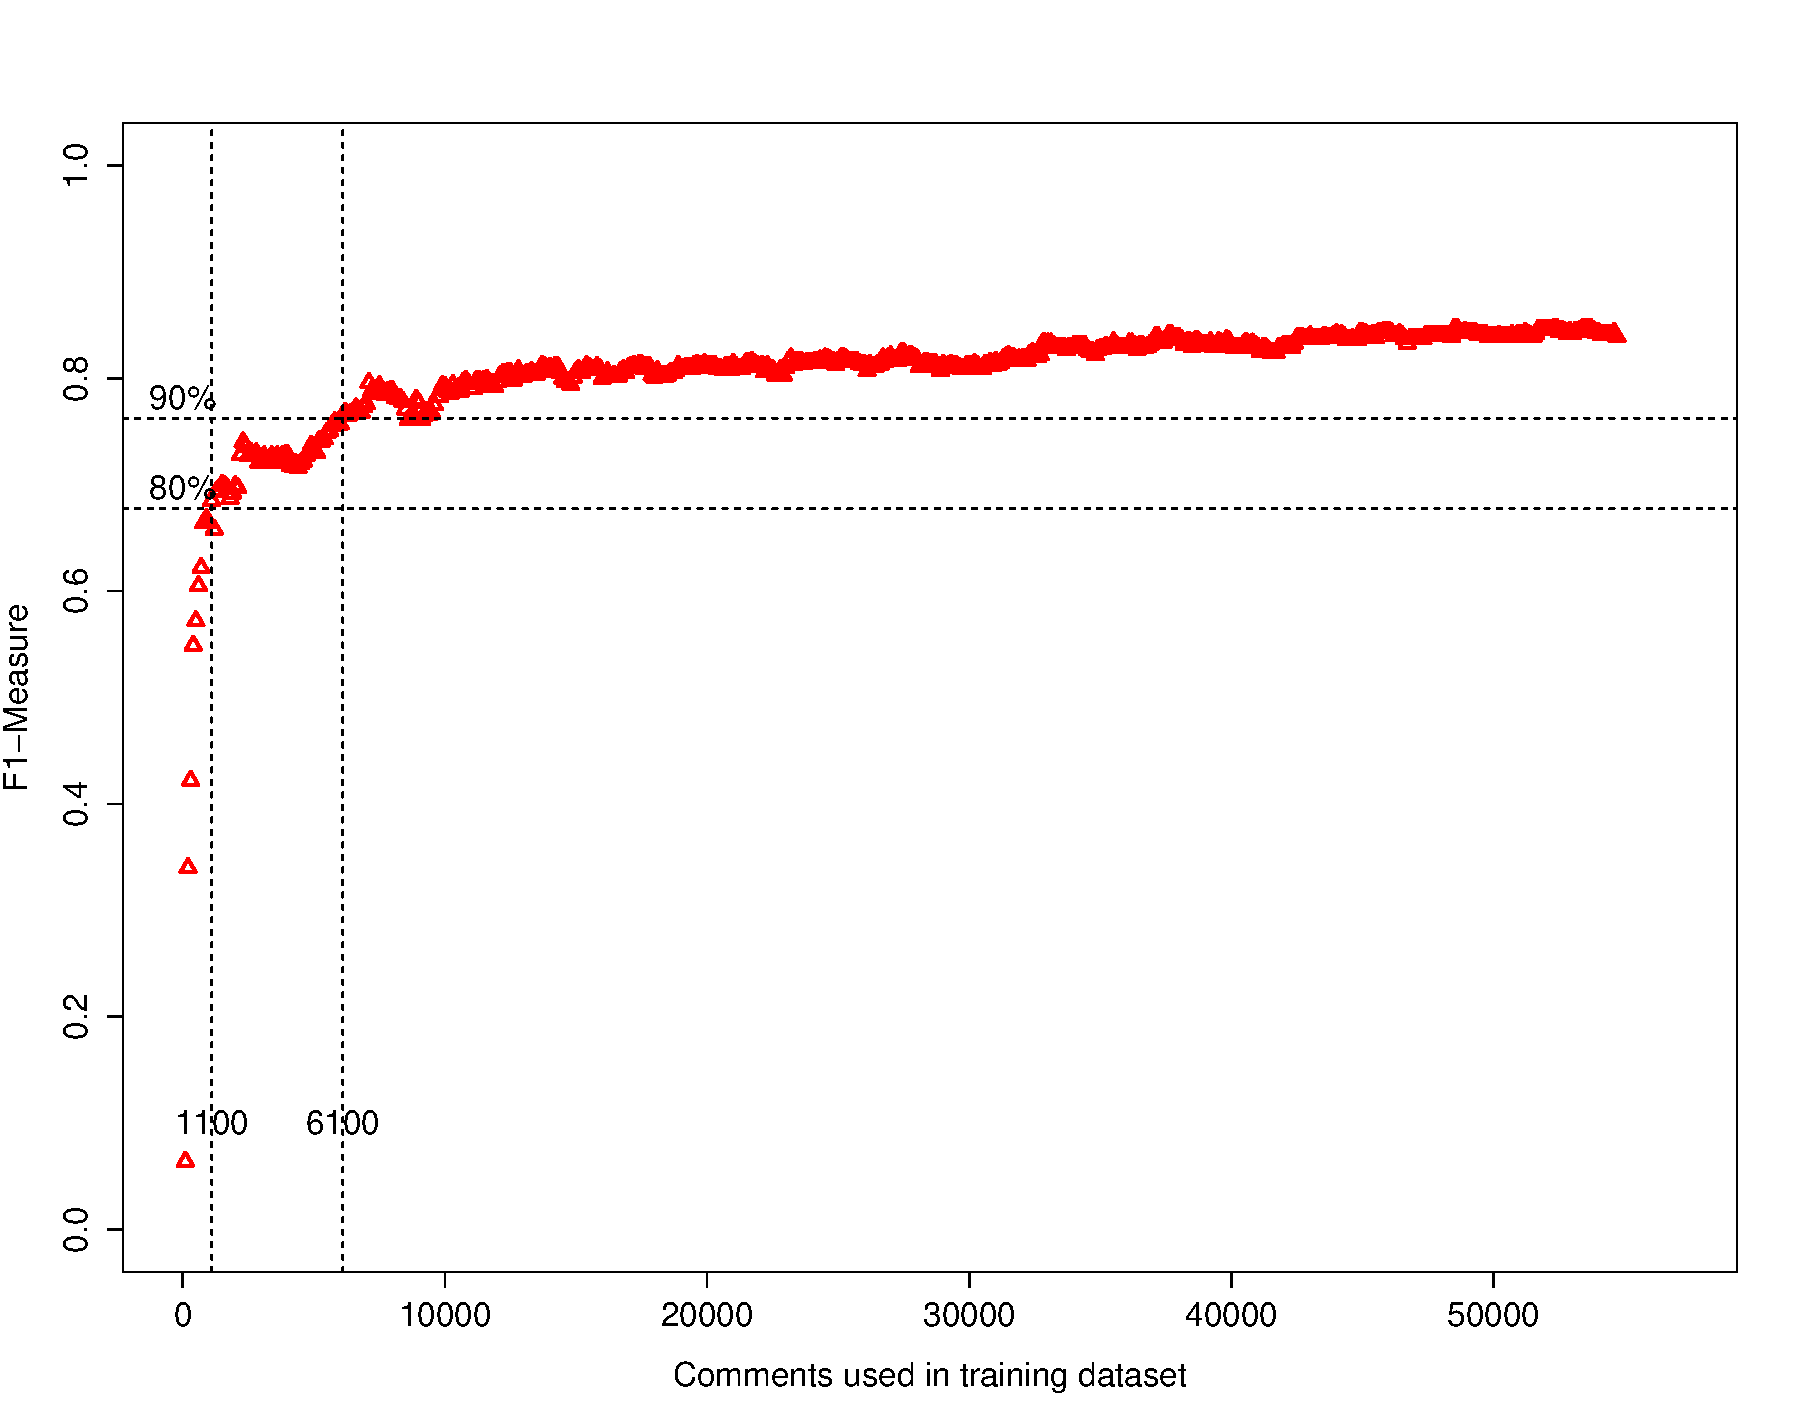
\includegraphics[width=0.49\textwidth]{figures/appendix/ten_fold_validation_design/ten_fold_validation_0_100.pdf}
  \vspace{-5mm}
  \caption{Ten Fold Validation Adding 100 Comments Per Time. First Iteration}
  \label{fig:design_ten_fold_validation_0_100}
  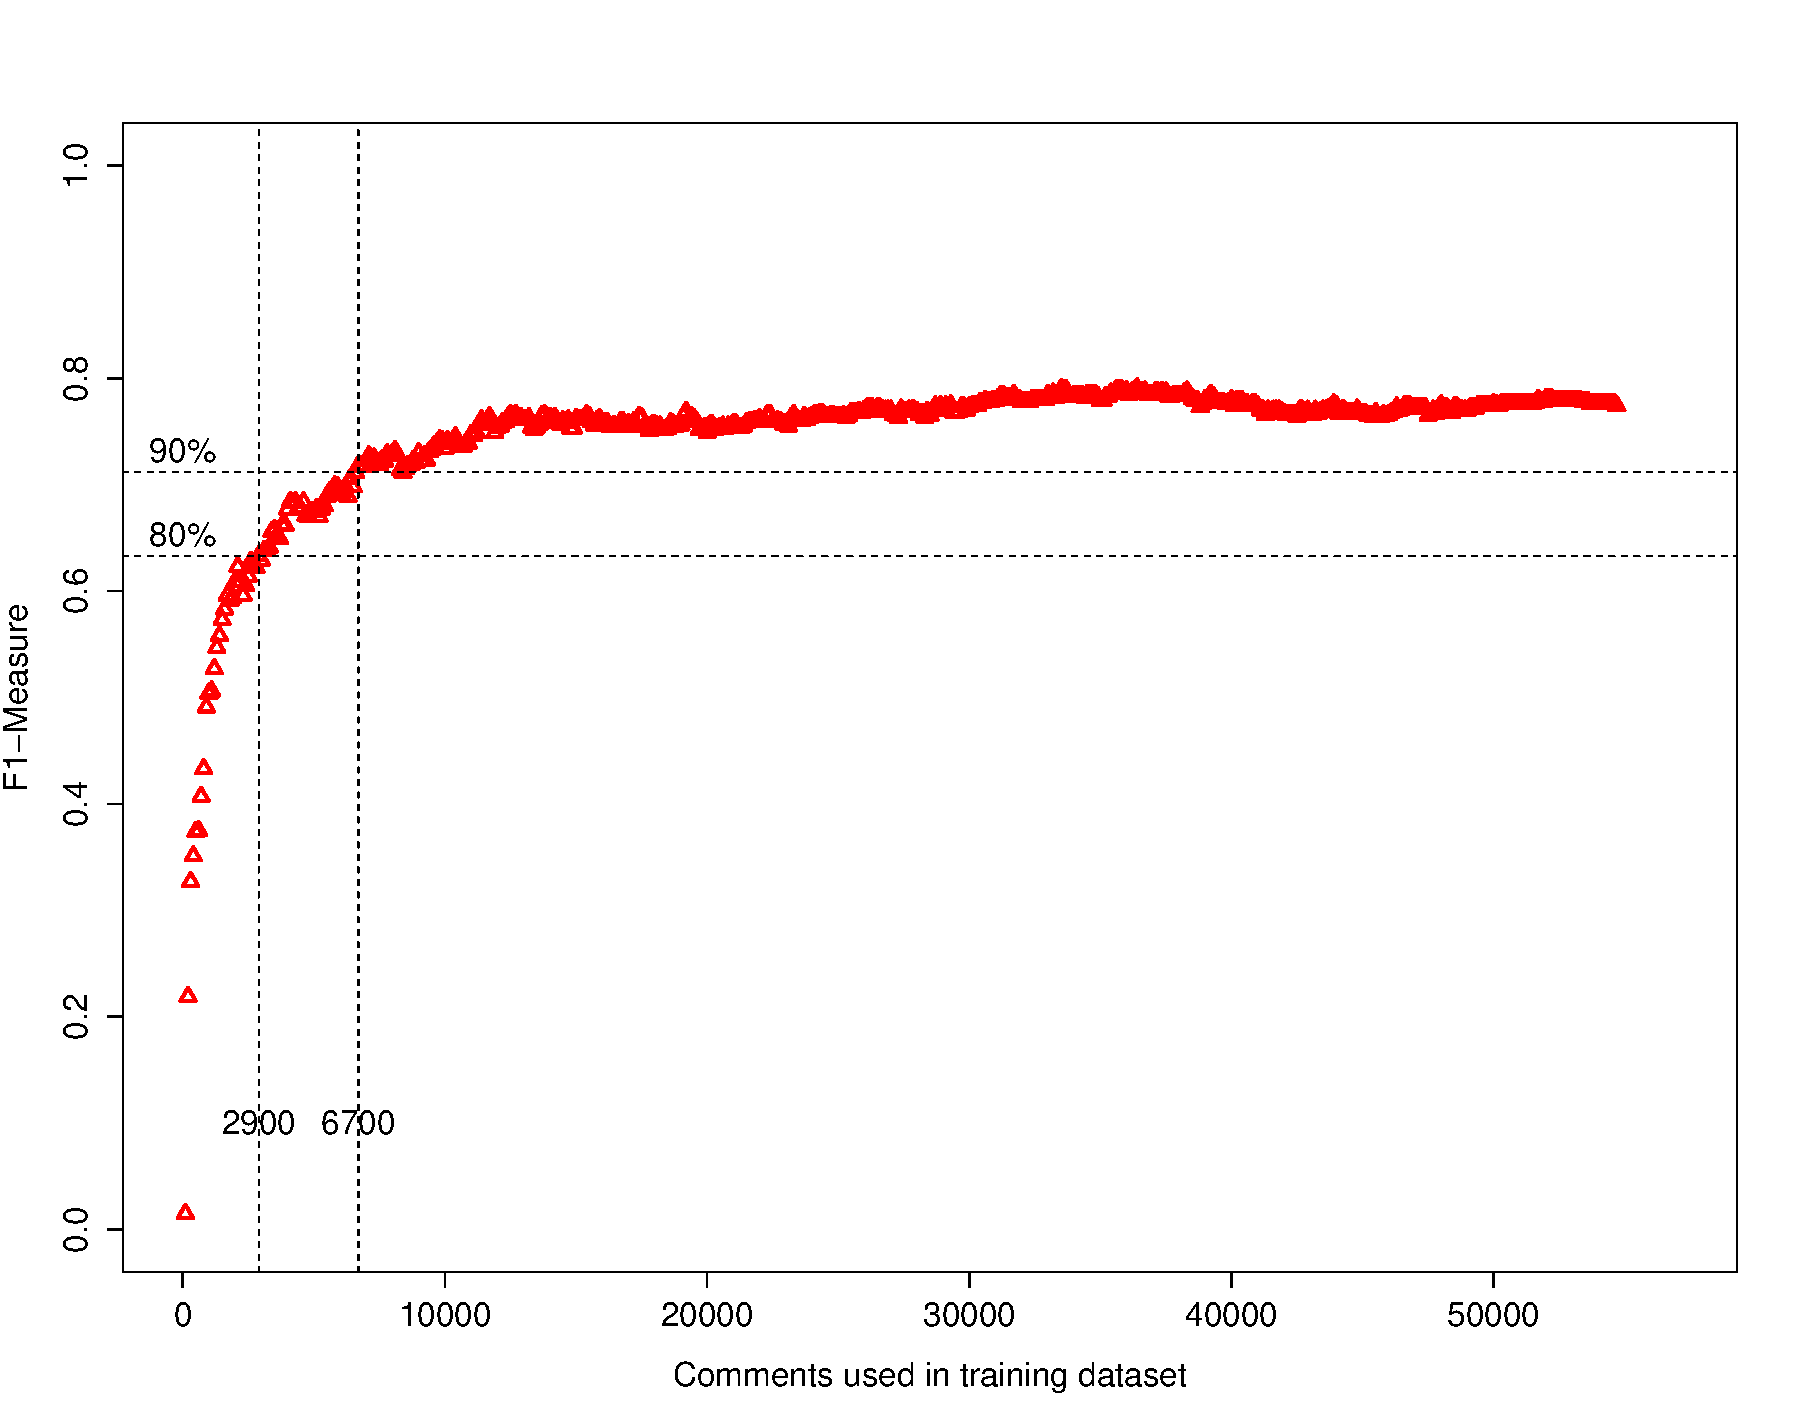
\includegraphics[width=0.49\textwidth]{figures/appendix/ten_fold_validation_design/ten_fold_validation_2_100.pdf}
  \vspace{-5mm}
  \caption{Ten Fold Validation Adding 100 Comments Per Time. Third Iteration}
  \label{fig:design_ten_fold_validation_2_100}
  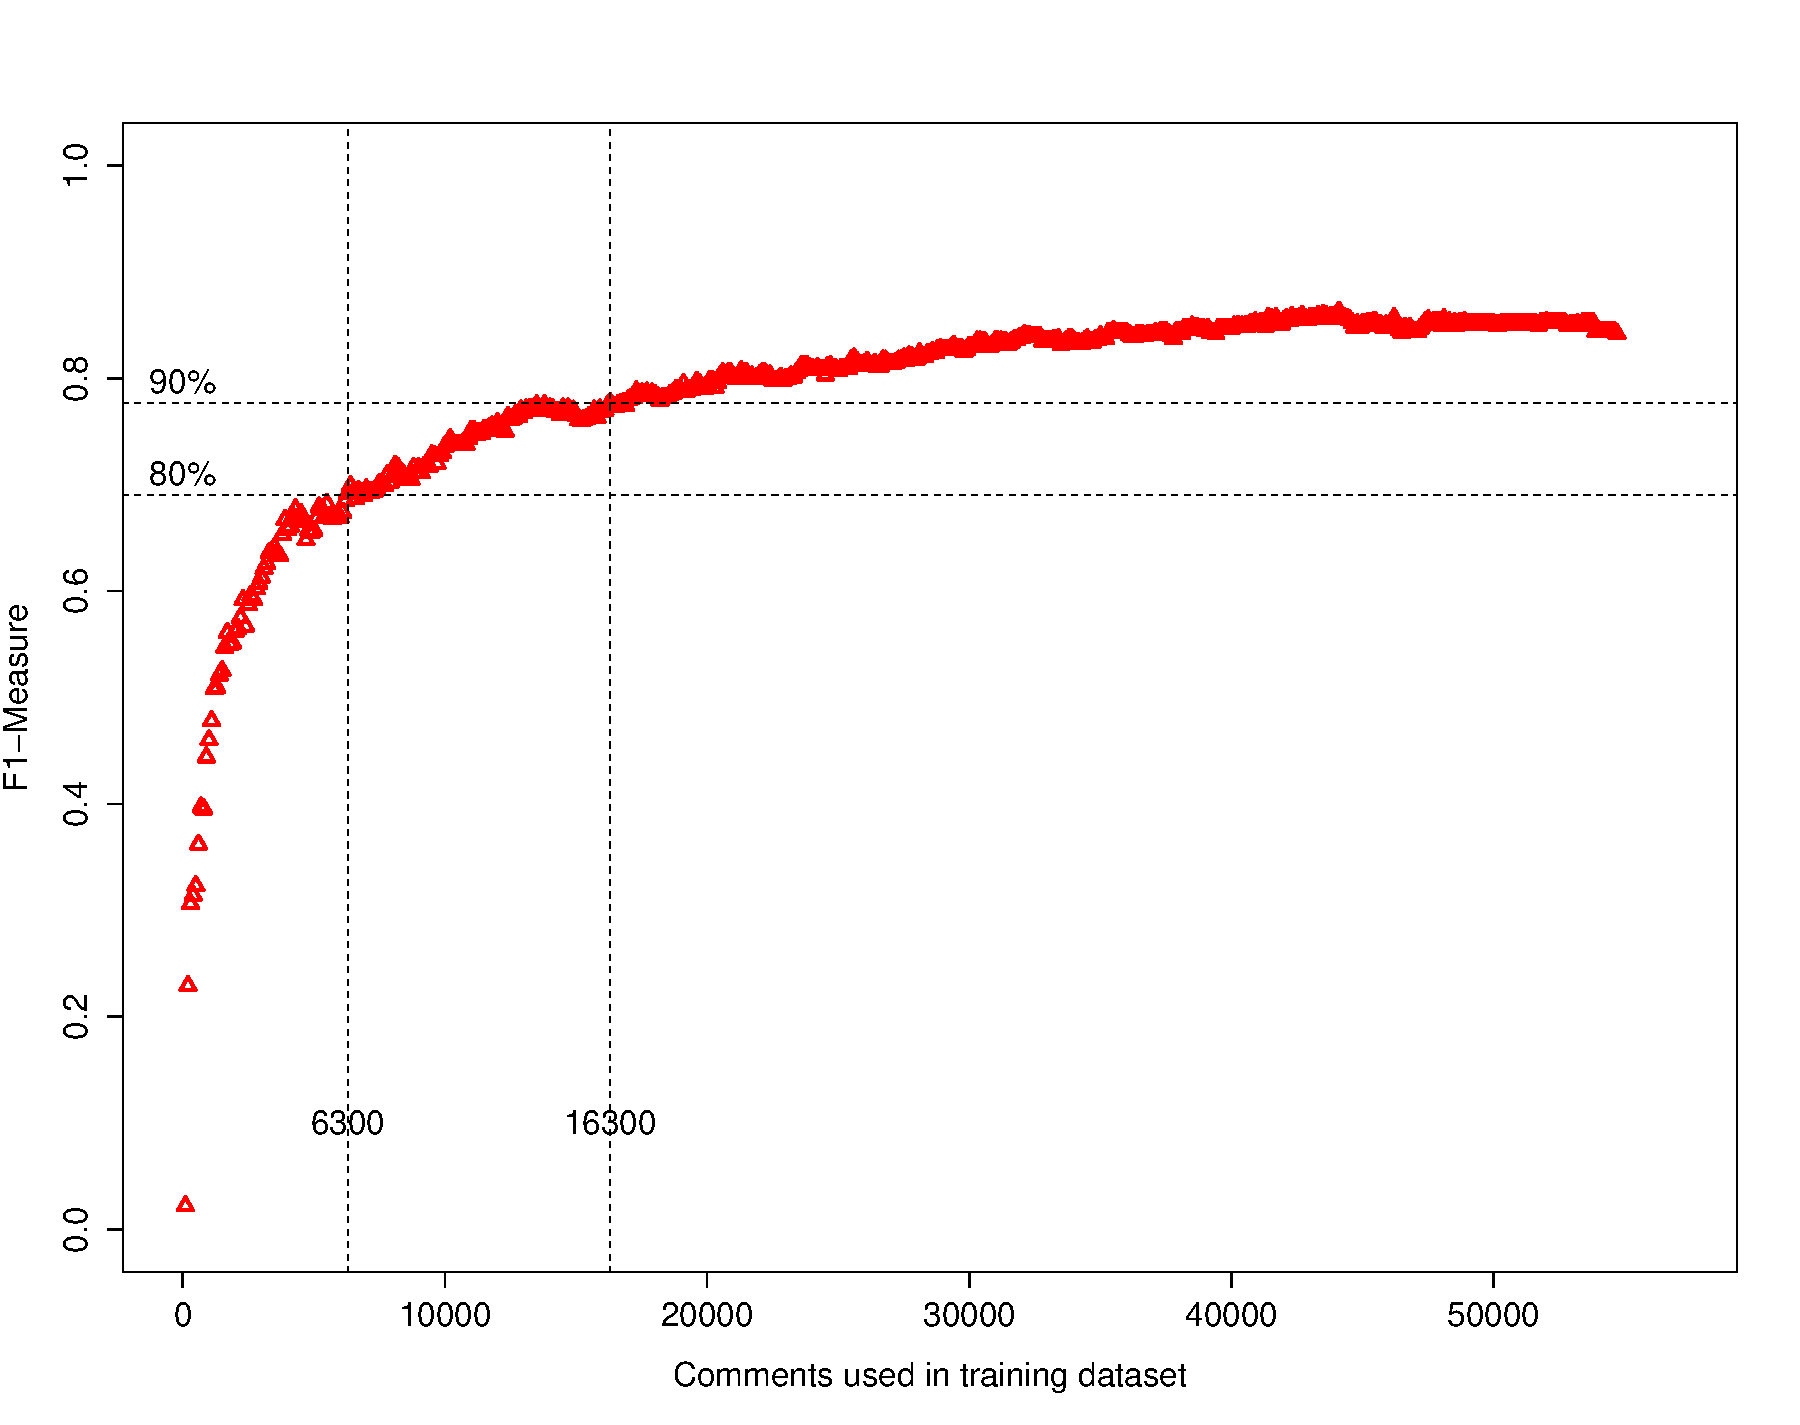
\includegraphics[width=0.49\textwidth]{figures/appendix/ten_fold_validation_design/ten_fold_validation_4_100.pdf}
  \vspace{-5mm}
  \caption{Ten Fold Validation Adding 100 Comments Per Time. Fifth Iteration}
  \label{fig:design_ten_fold_validation_4_100}
\end{figure}

\begin{figure}[thb!]
  \centering
  \vspace{-14mm}
  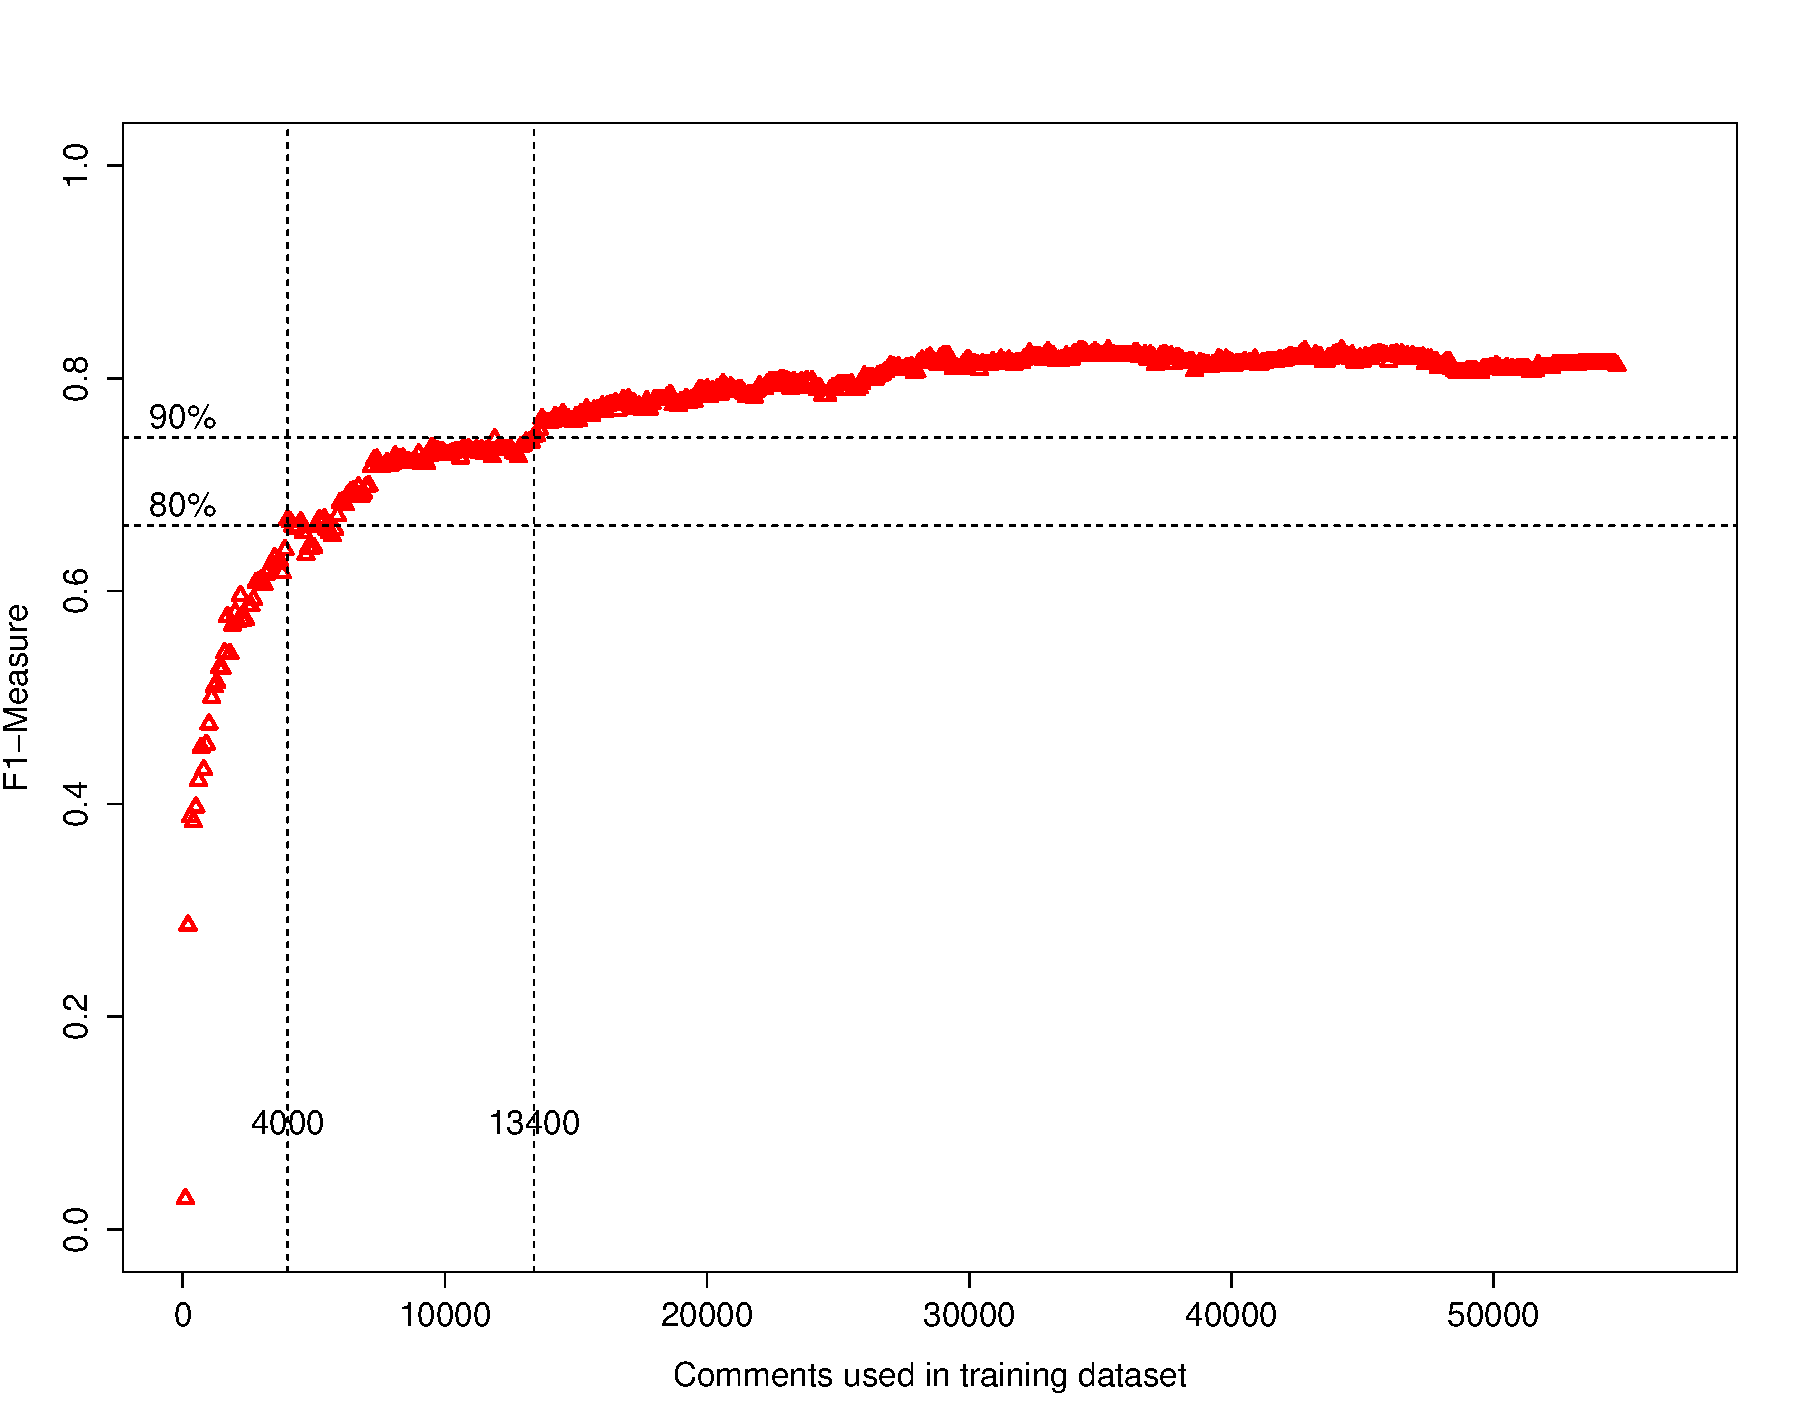
\includegraphics[width=0.49\textwidth]{figures/appendix/ten_fold_validation_design/ten_fold_validation_1_100.pdf}
  \vspace{-5mm}
  \caption{Ten Fold Validation Adding 100 Comments Per Time. Second Iteration}
  \label{fig:design_ten_fold_validation_1_100}
  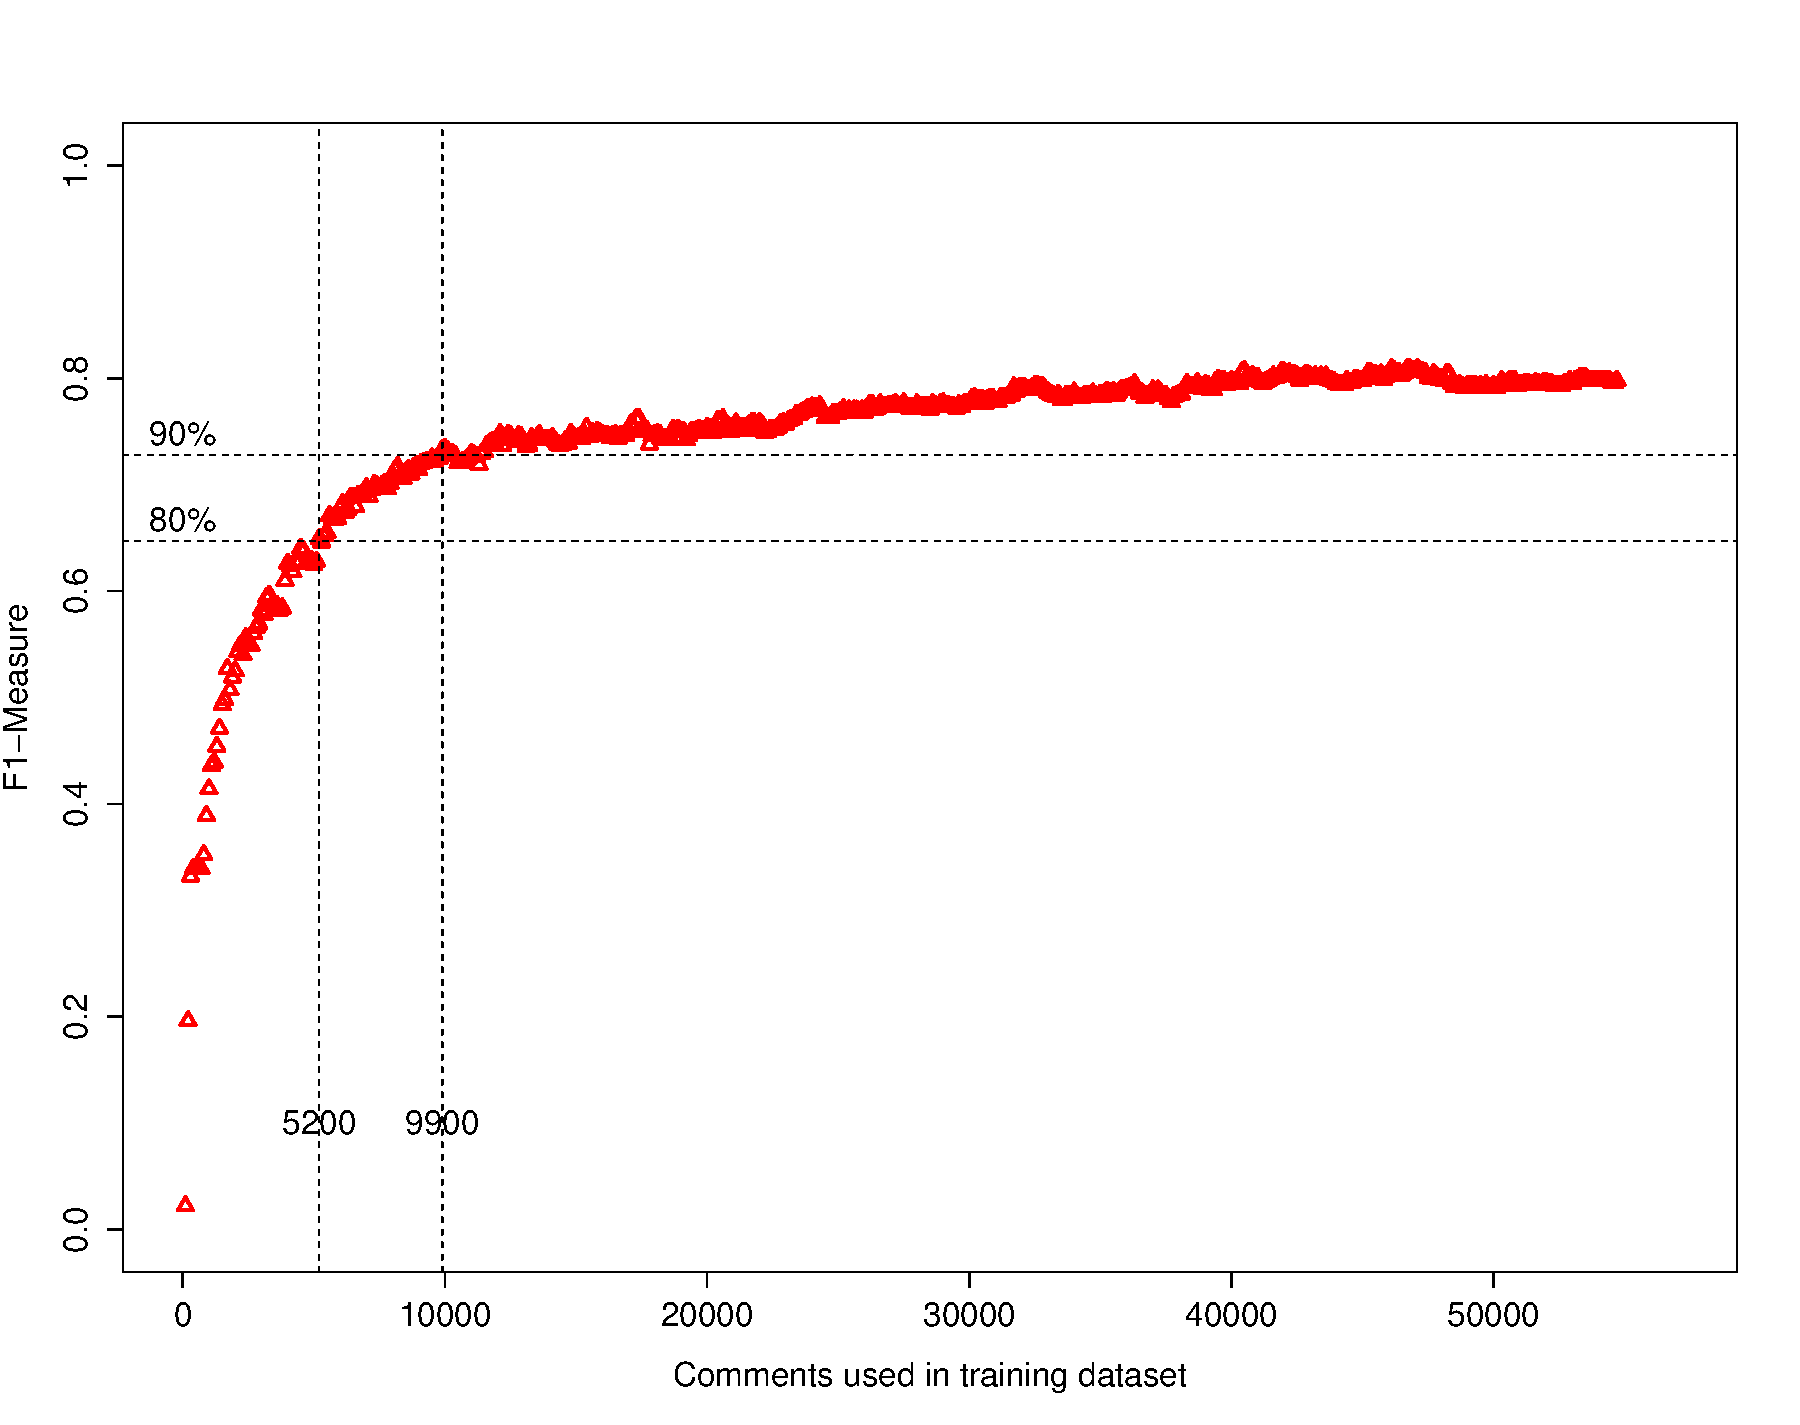
\includegraphics[width=0.49\textwidth]{figures/appendix/ten_fold_validation_design/ten_fold_validation_3_100.pdf}
  \vspace{-5mm}
  \caption{Ten Fold Validation Adding 100 Comments Per Time. Fourth Iteration}
  \label{fig:design_ten_fold_validation_3_100}
  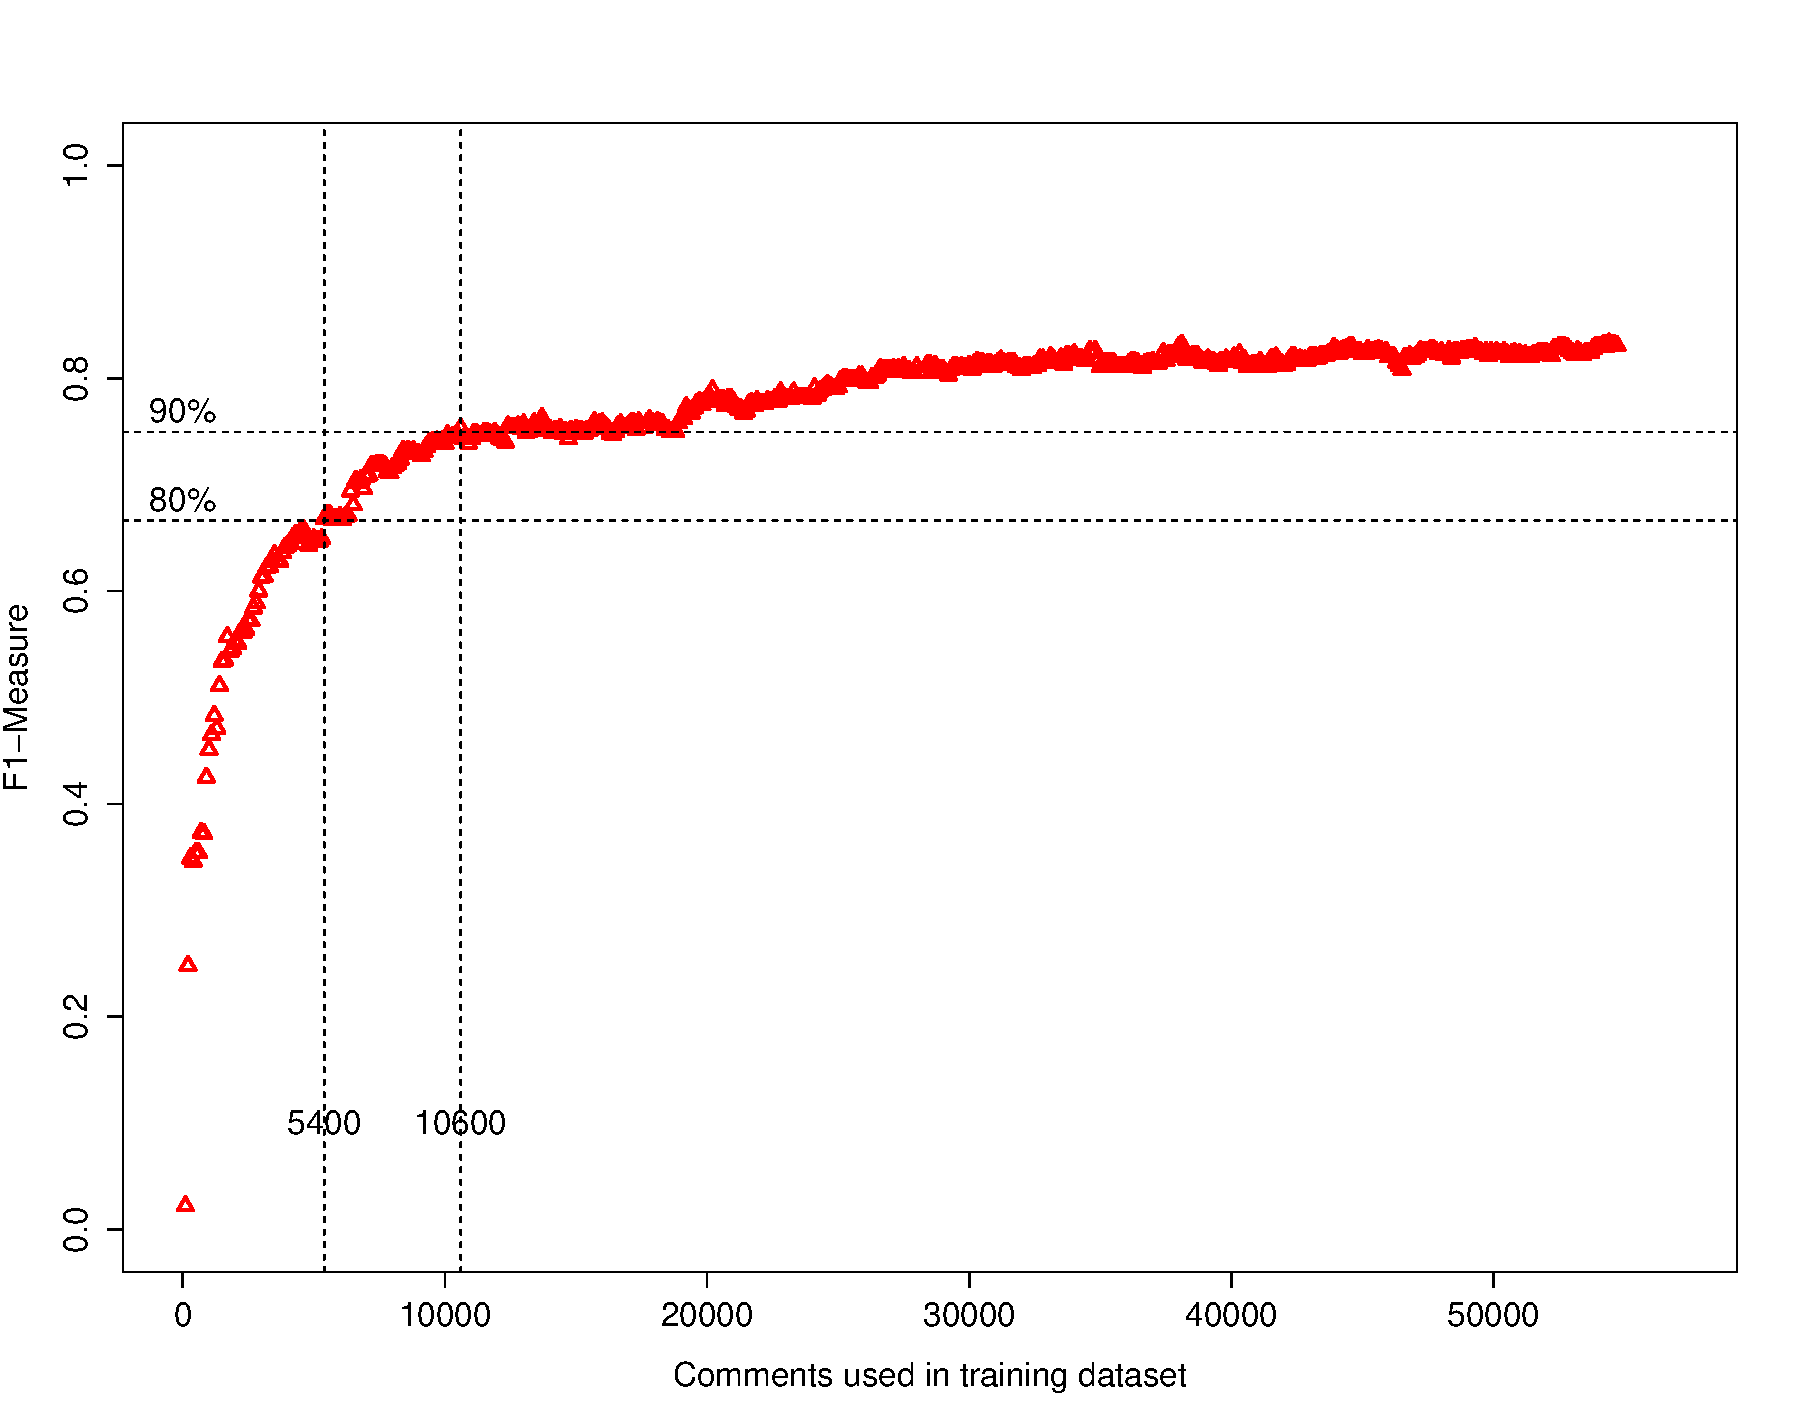
\includegraphics[width=0.49\textwidth]{figures/appendix/ten_fold_validation_design/ten_fold_validation_5_100.pdf}
  \vspace{-5mm}
  \caption{Ten Fold Validation Adding 100 Comments Per Time. Sixth Iteration}
  \label{fig:design_ten_fold_validation_5_100}
\end{figure}

\clearpage
\begin{figure}[thb!]
  \centering
  \vspace{-3mm}
  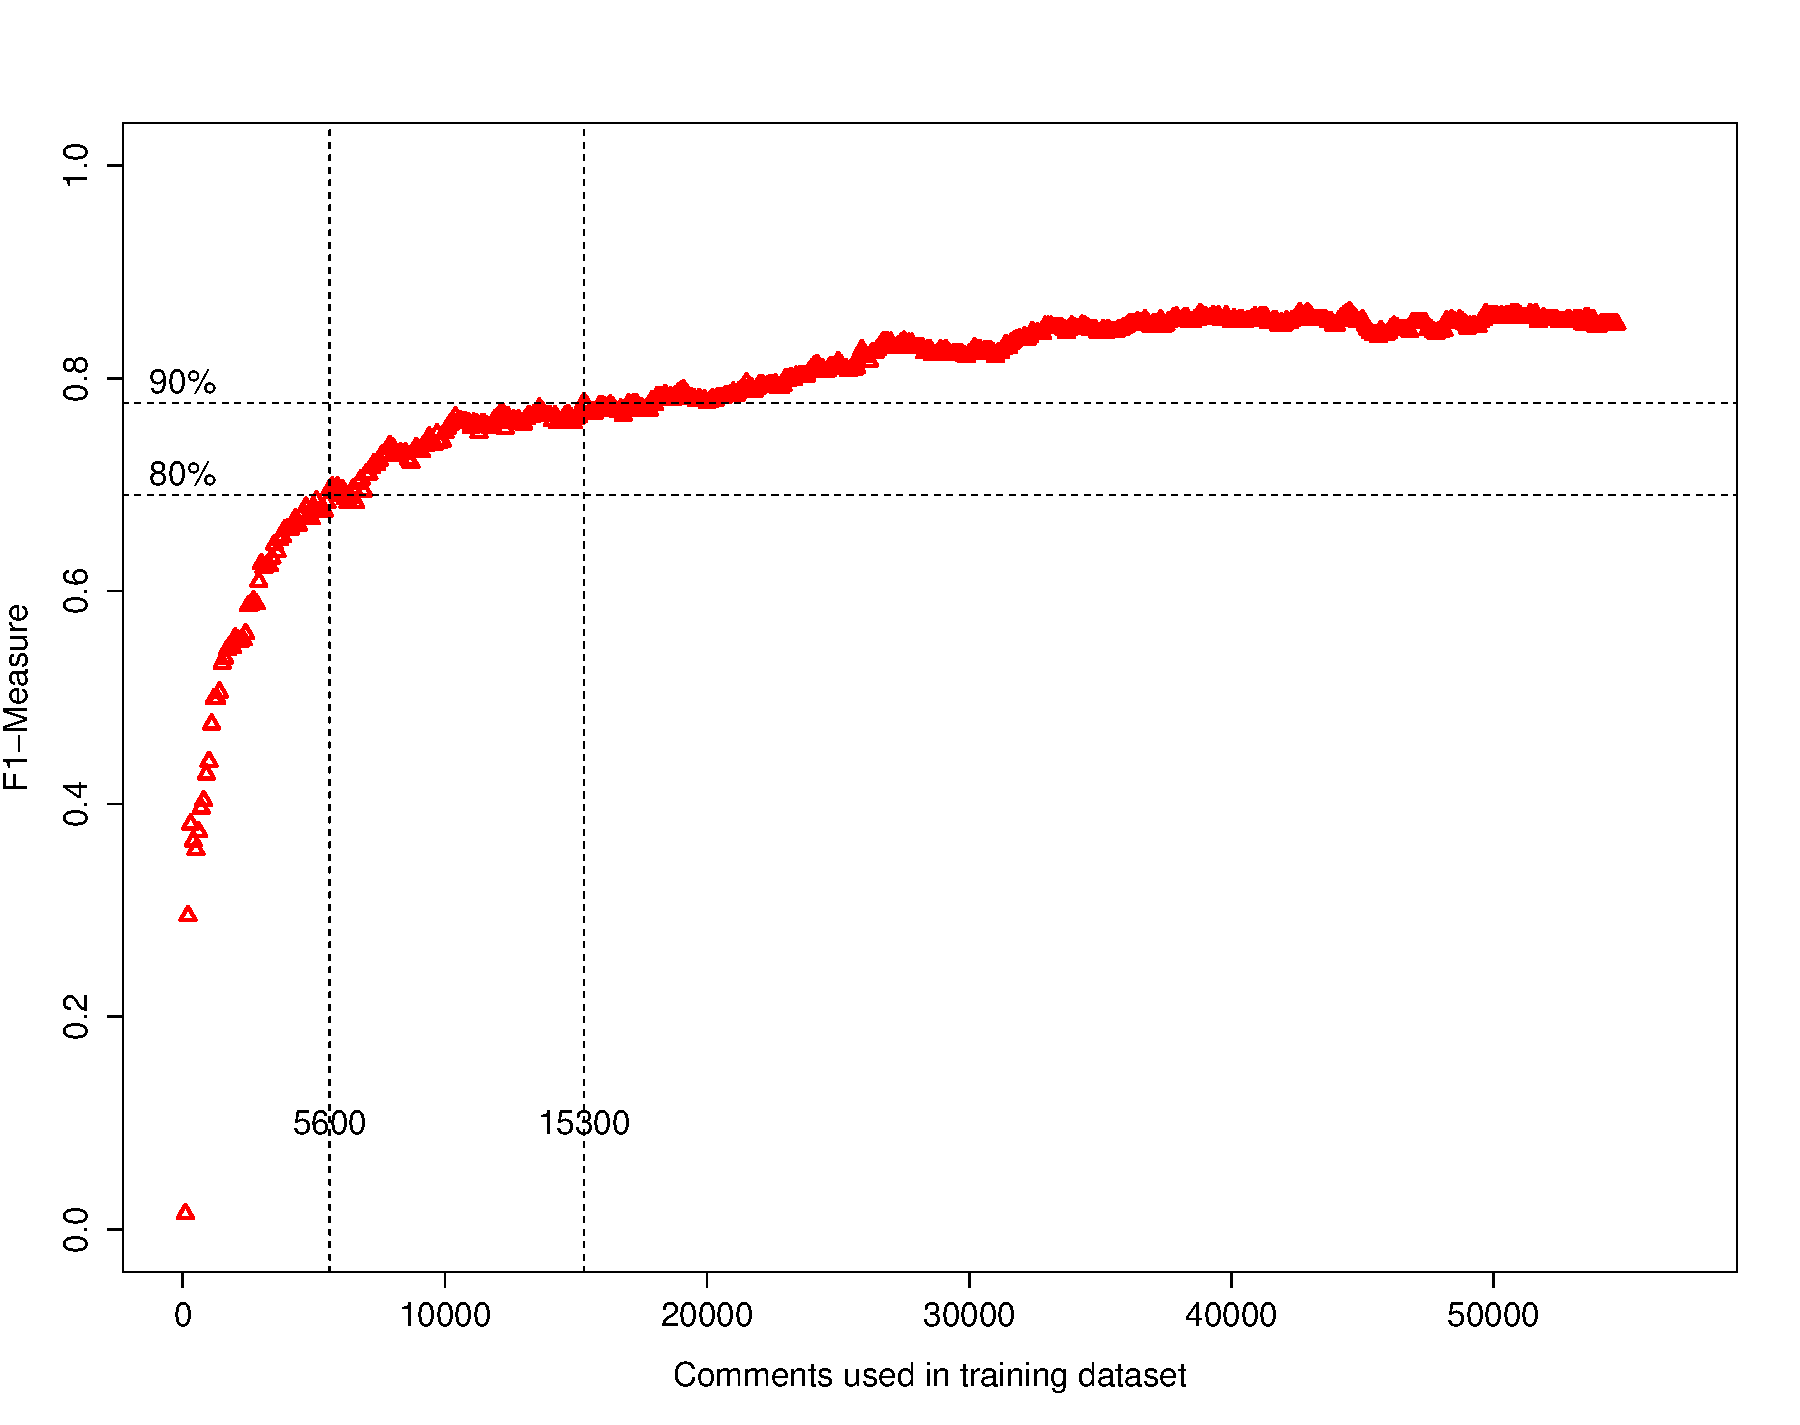
\includegraphics[width=0.49\textwidth]{figures/appendix/ten_fold_validation_design/ten_fold_validation_6_100.pdf}
  \vspace{-5mm}
  \caption{Ten Fold Validation Adding 100 Comments Per Time. Seventh Iteration}
  \label{fig:design_ten_fold_validation_6_100}
  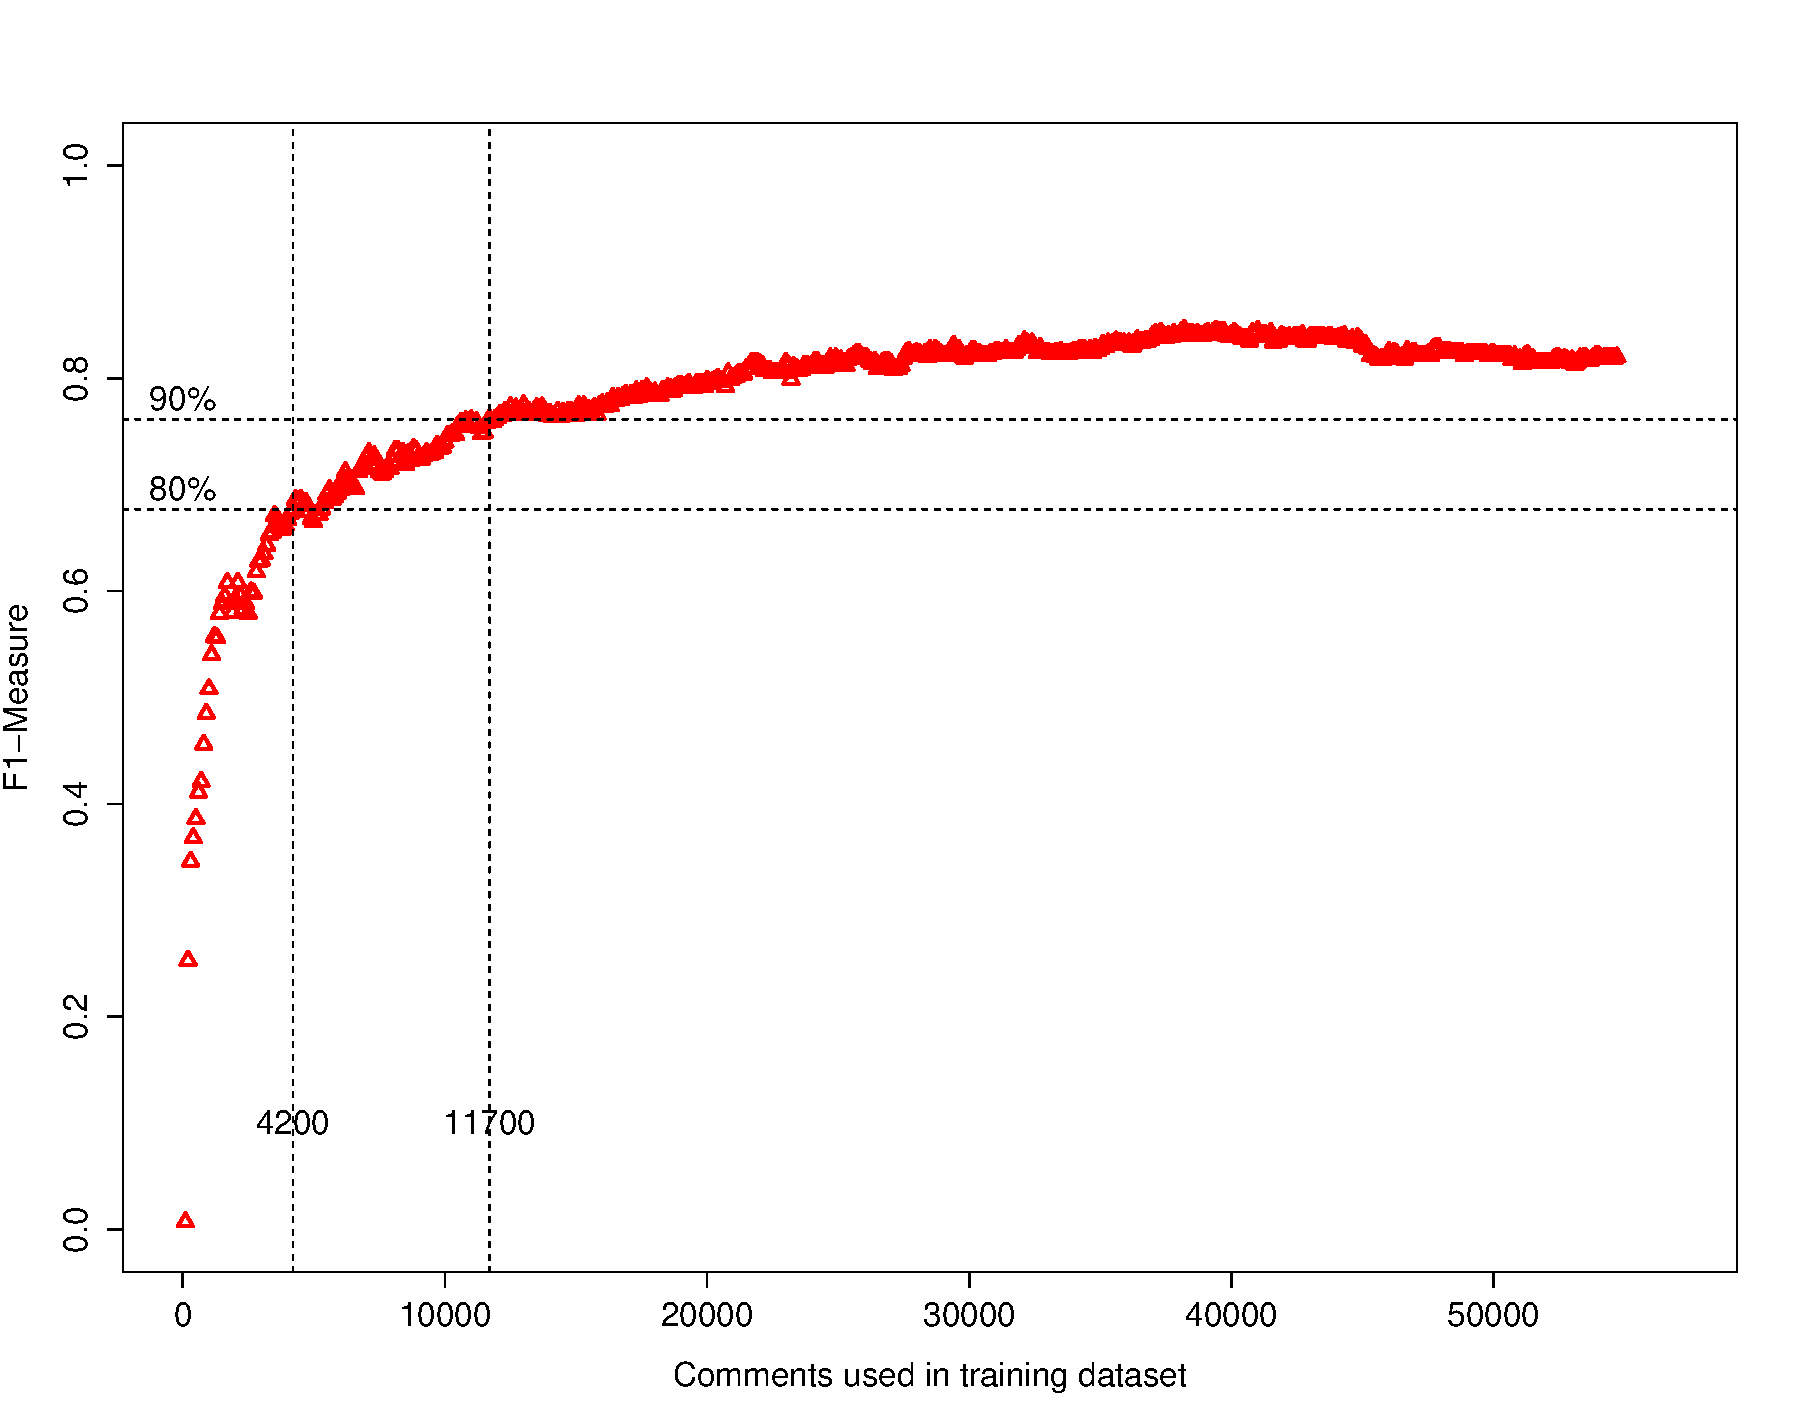
\includegraphics[width=0.49\textwidth]{figures/appendix/ten_fold_validation_design/ten_fold_validation_8_100.pdf}
  \vspace{-5mm}
  \caption{Ten Fold Validation Adding 100 Comments Per Time. Ninth Iteration}
  \label{fig:design_ten_fold_validation_8_100}
  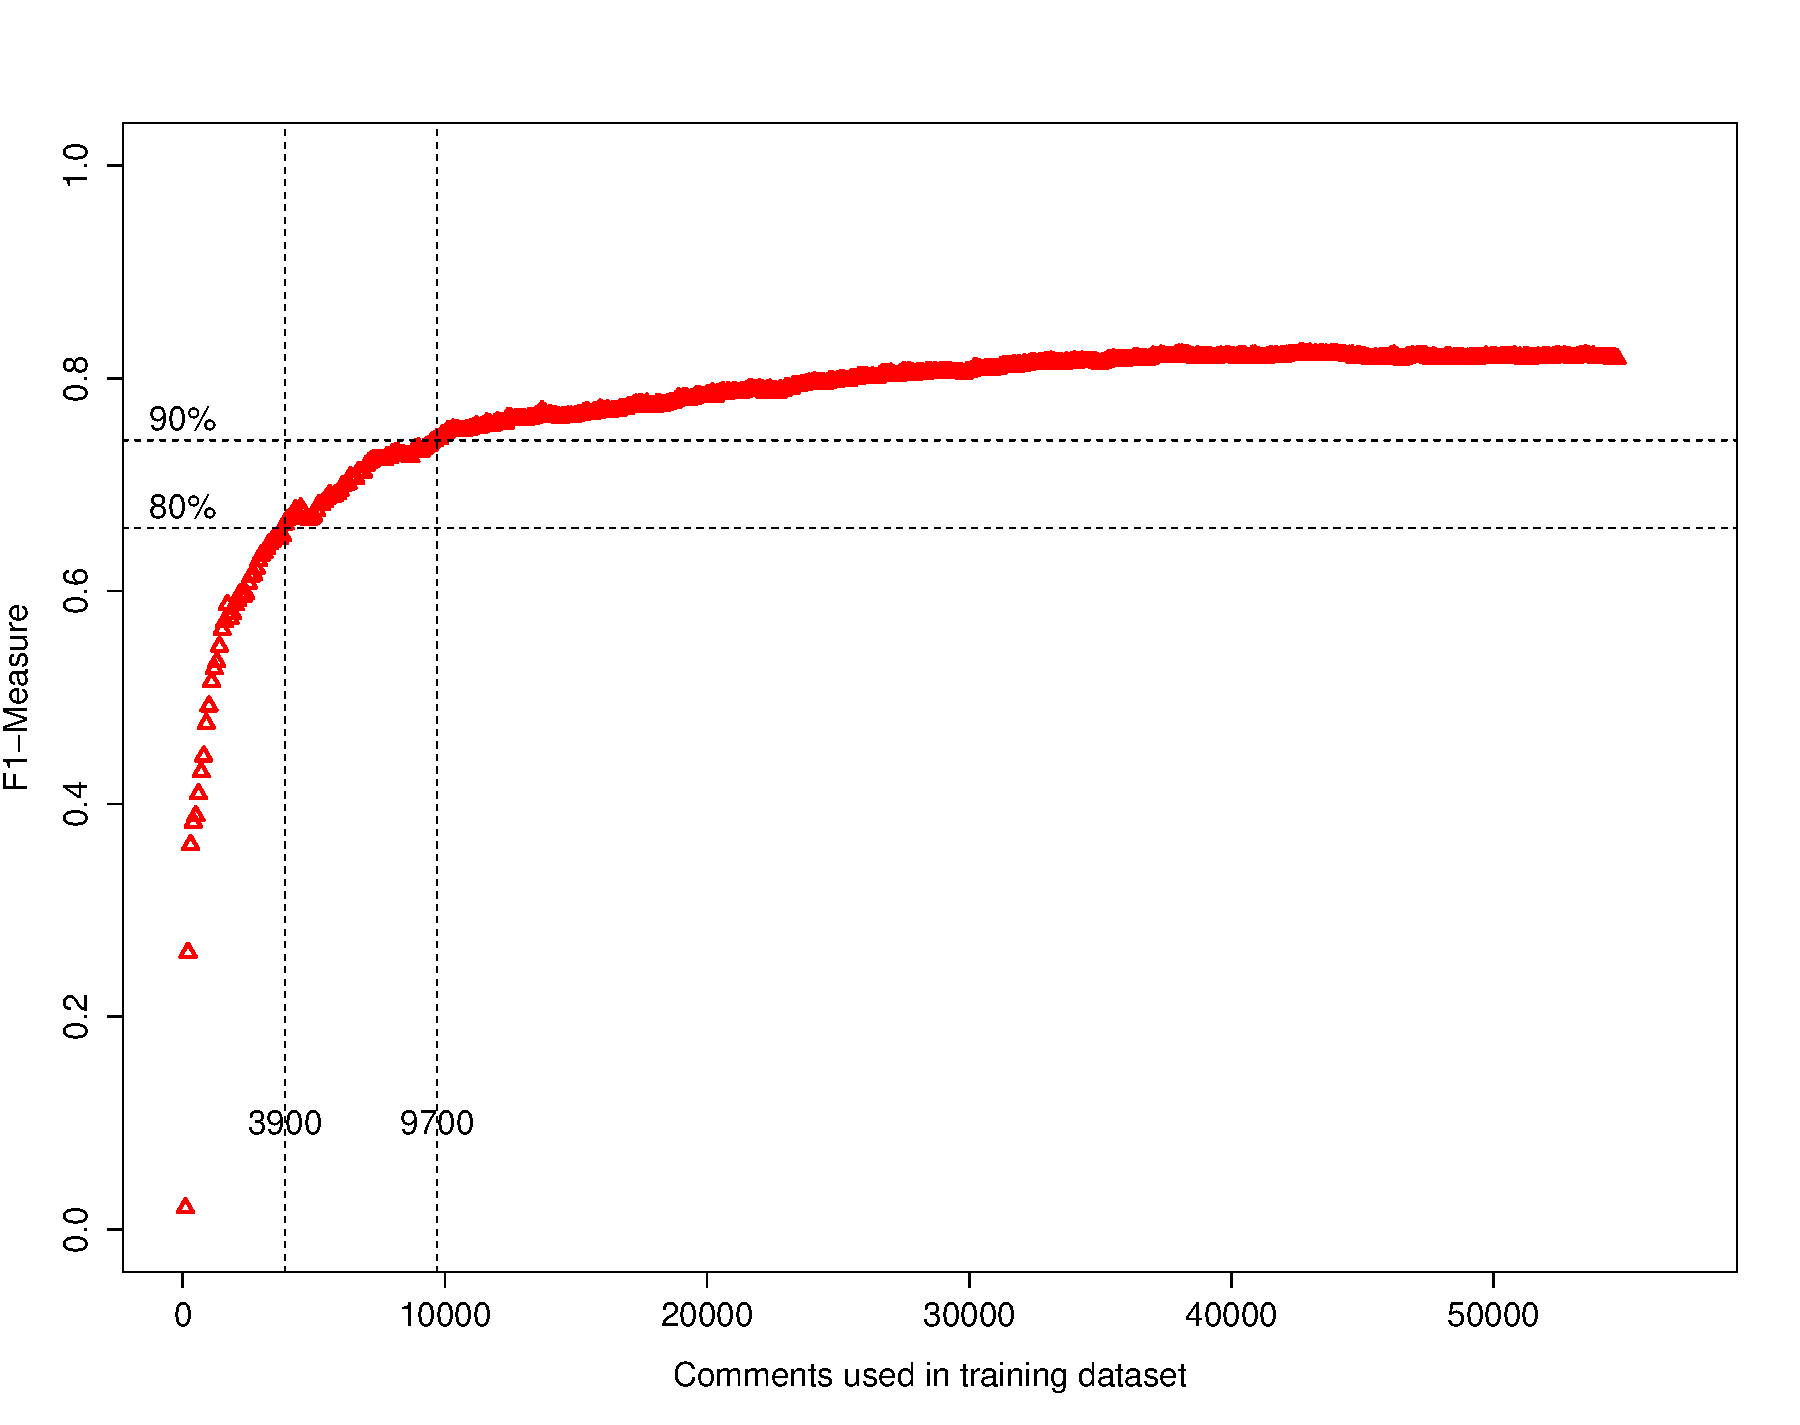
\includegraphics[width=0.49\textwidth]{figures/appendix/ten_fold_validation_design/ten_fold_validation_average_100.pdf}
  \vspace{-5mm}
  \caption{Ten Fold Validation Adding 100 Comments Per Time. Average}
  \label{fig:design_ten_fold_validation_average_100}
\end{figure}

\begin{figure}[thb!]
  \centering
  \vspace{-93mm}
  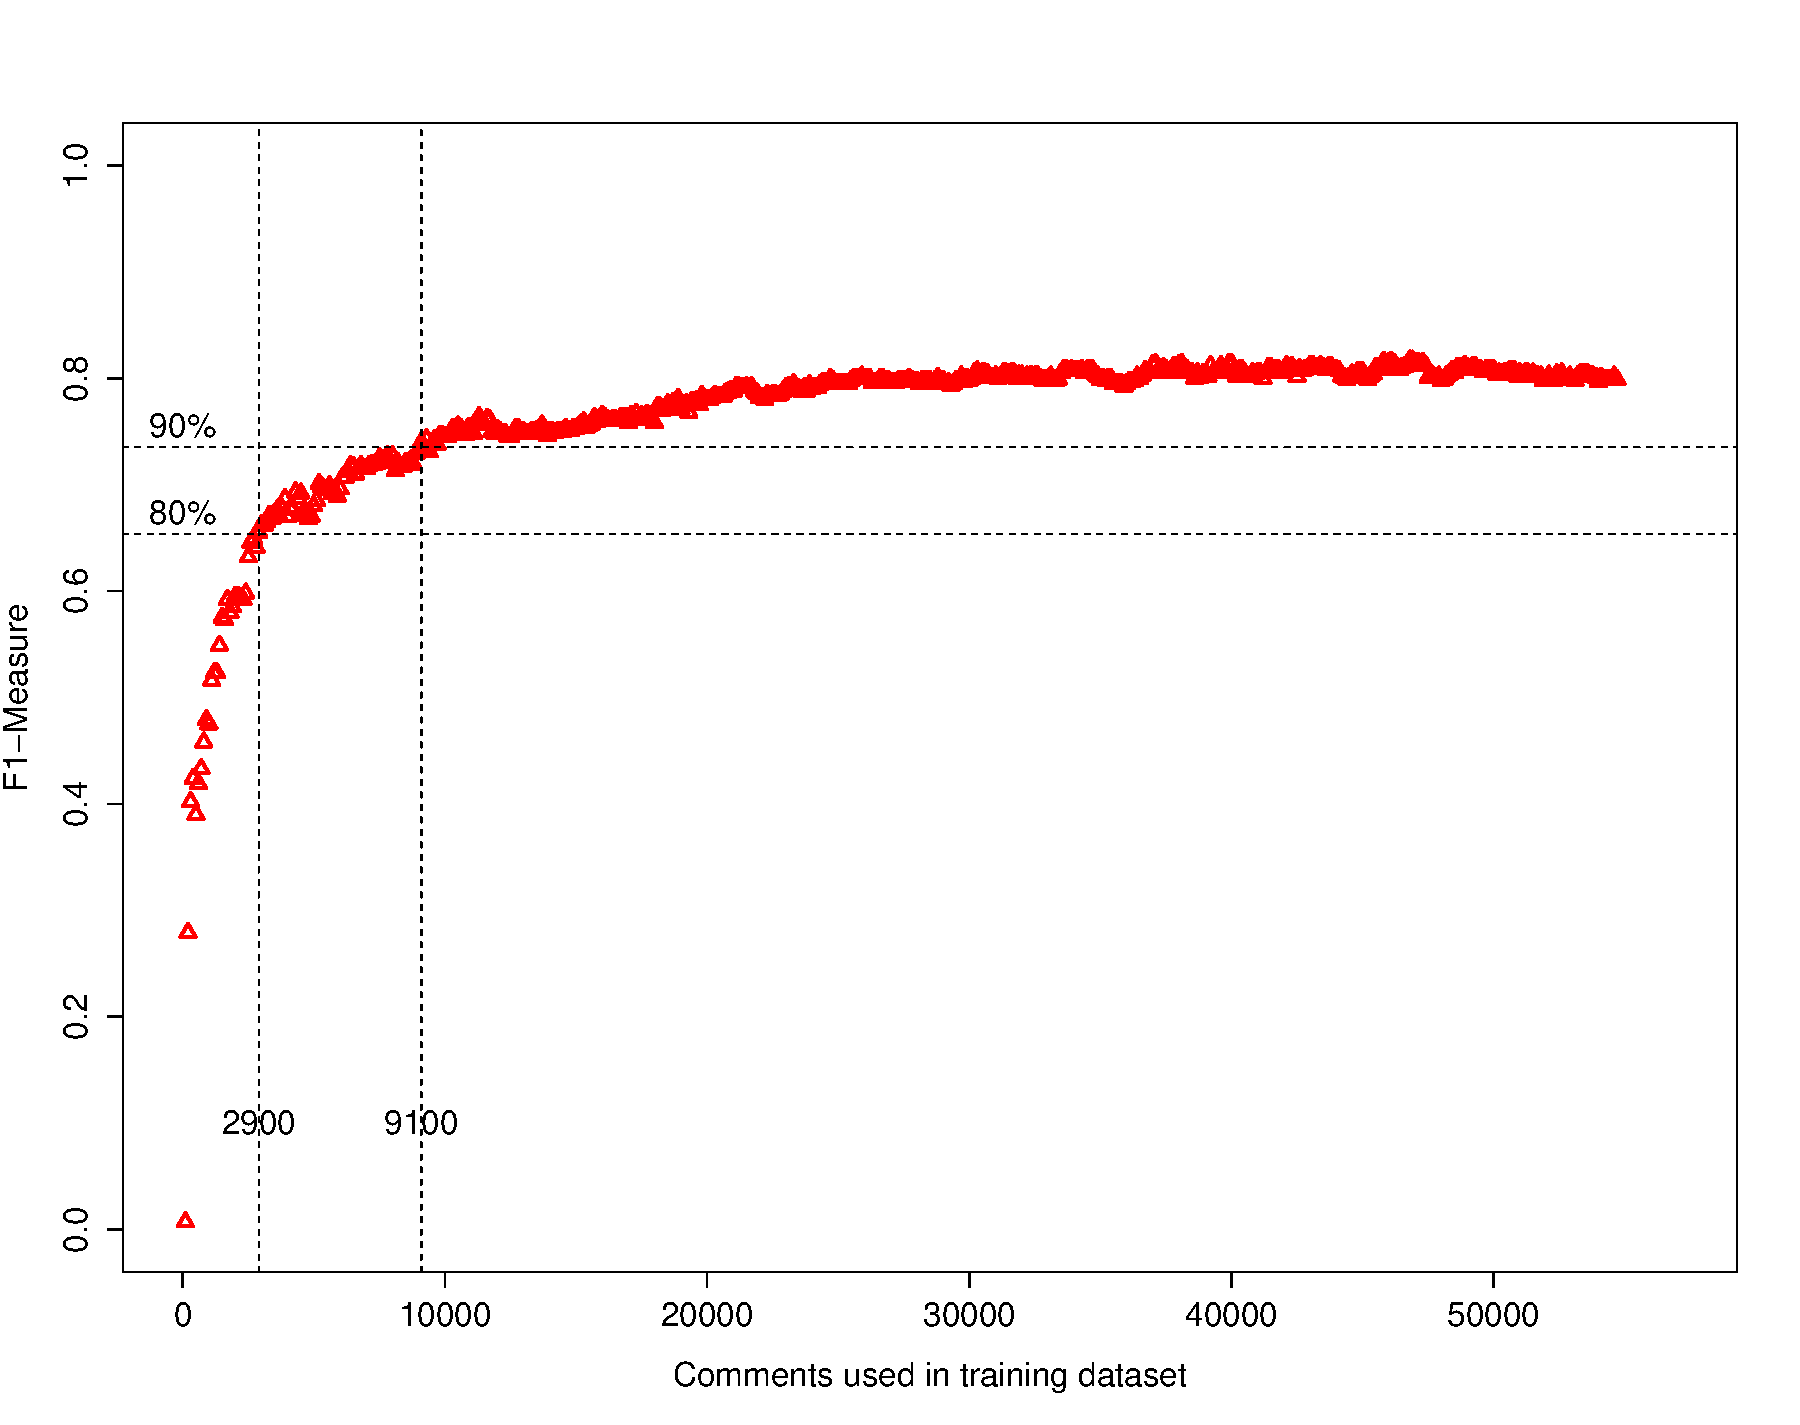
\includegraphics[width=0.49\textwidth]{figures/appendix/ten_fold_validation_design/ten_fold_validation_7_100.pdf}
  \vspace{-5mm}
  \caption{Ten Fold Validation Adding 100 Comments Per Time. Eight Iteration}
  \label{fig:design_ten_fold_validation_7_100}
  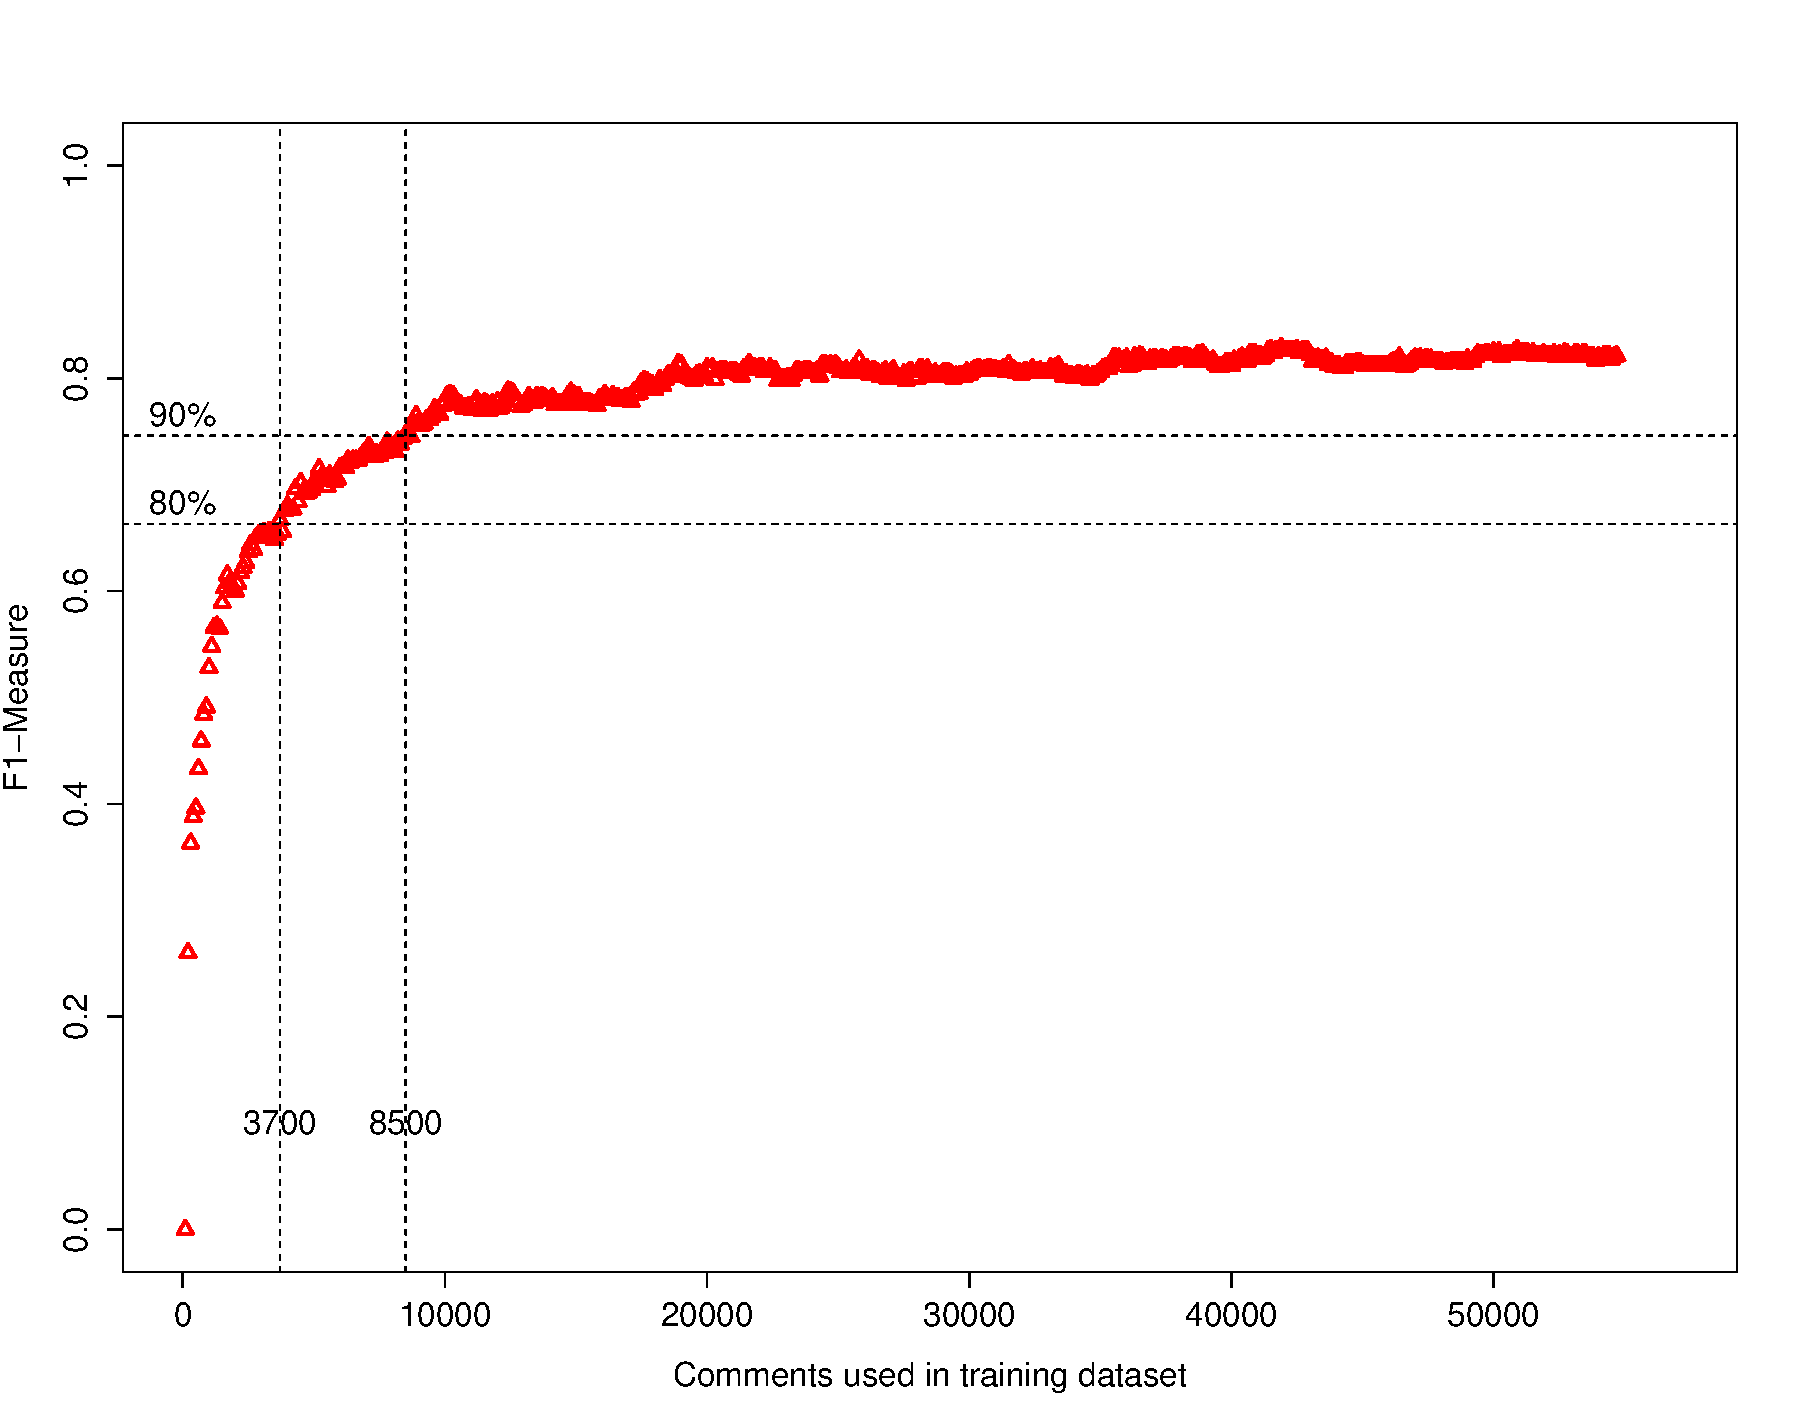
\includegraphics[width=0.49\textwidth]{figures/appendix/ten_fold_validation_design/ten_fold_validation_9_100.pdf}
  \vspace{-5mm}
  \caption{Ten Fold Validation Adding 100 Comments Per Time. Tenth Iteration}
  \label{fig:design_ten_fold_validation_9_100}
  
\end{figure}

\clearpage
\begin{figure}[thb!]
  \centering
  \vspace{-3mm}
  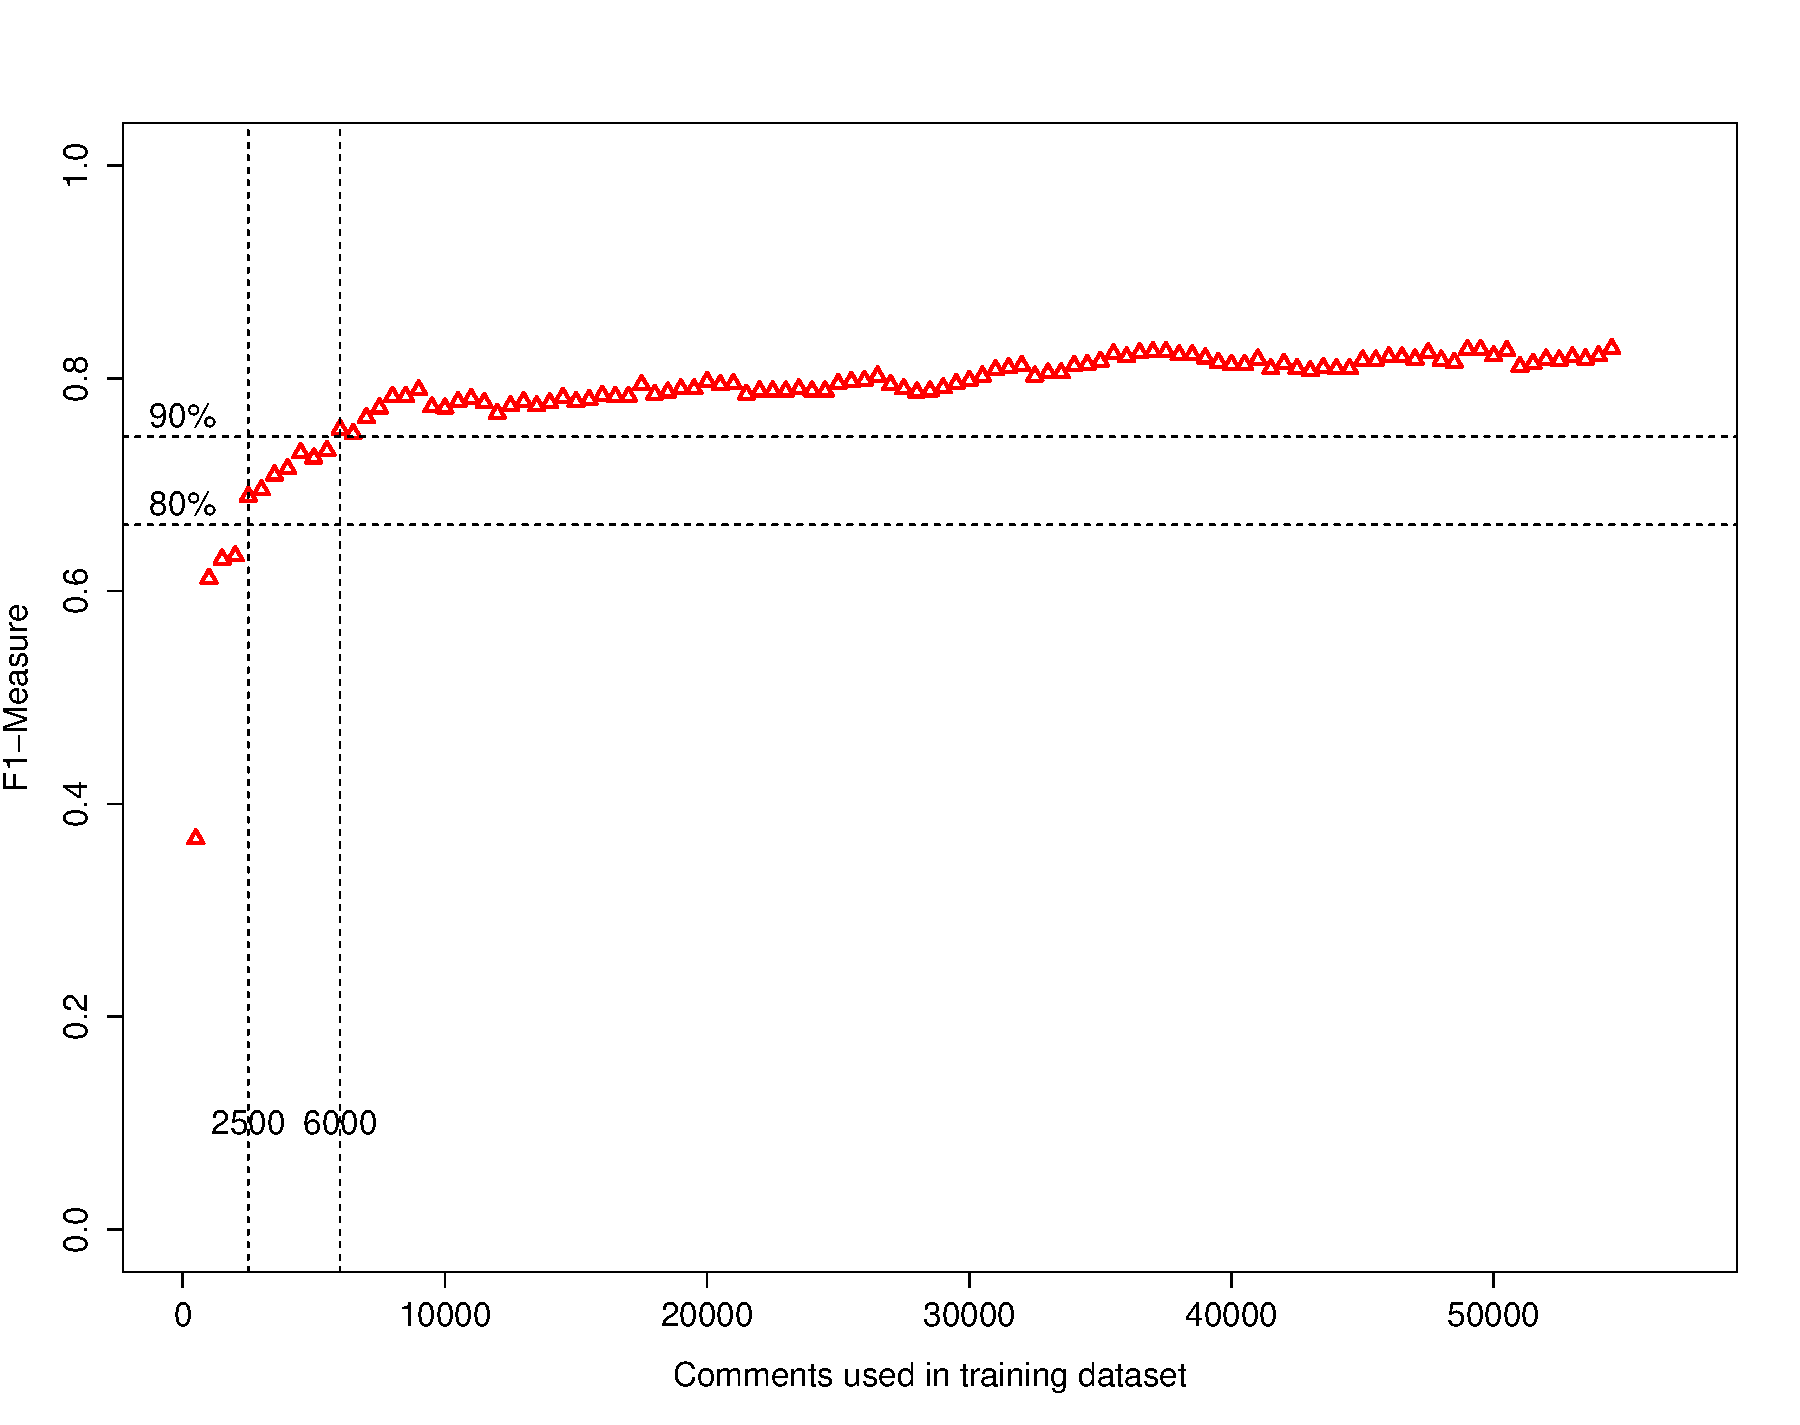
\includegraphics[width=0.49\textwidth]{figures/appendix/ten_fold_validation_design/ten_fold_validation_0_500.pdf}
  \vspace{-5mm}
  \caption{Ten Fold Validation Adding 500 Comments Per Time. First Iteration}
  \label{fig:design_ten_fold_validation_0_100}
  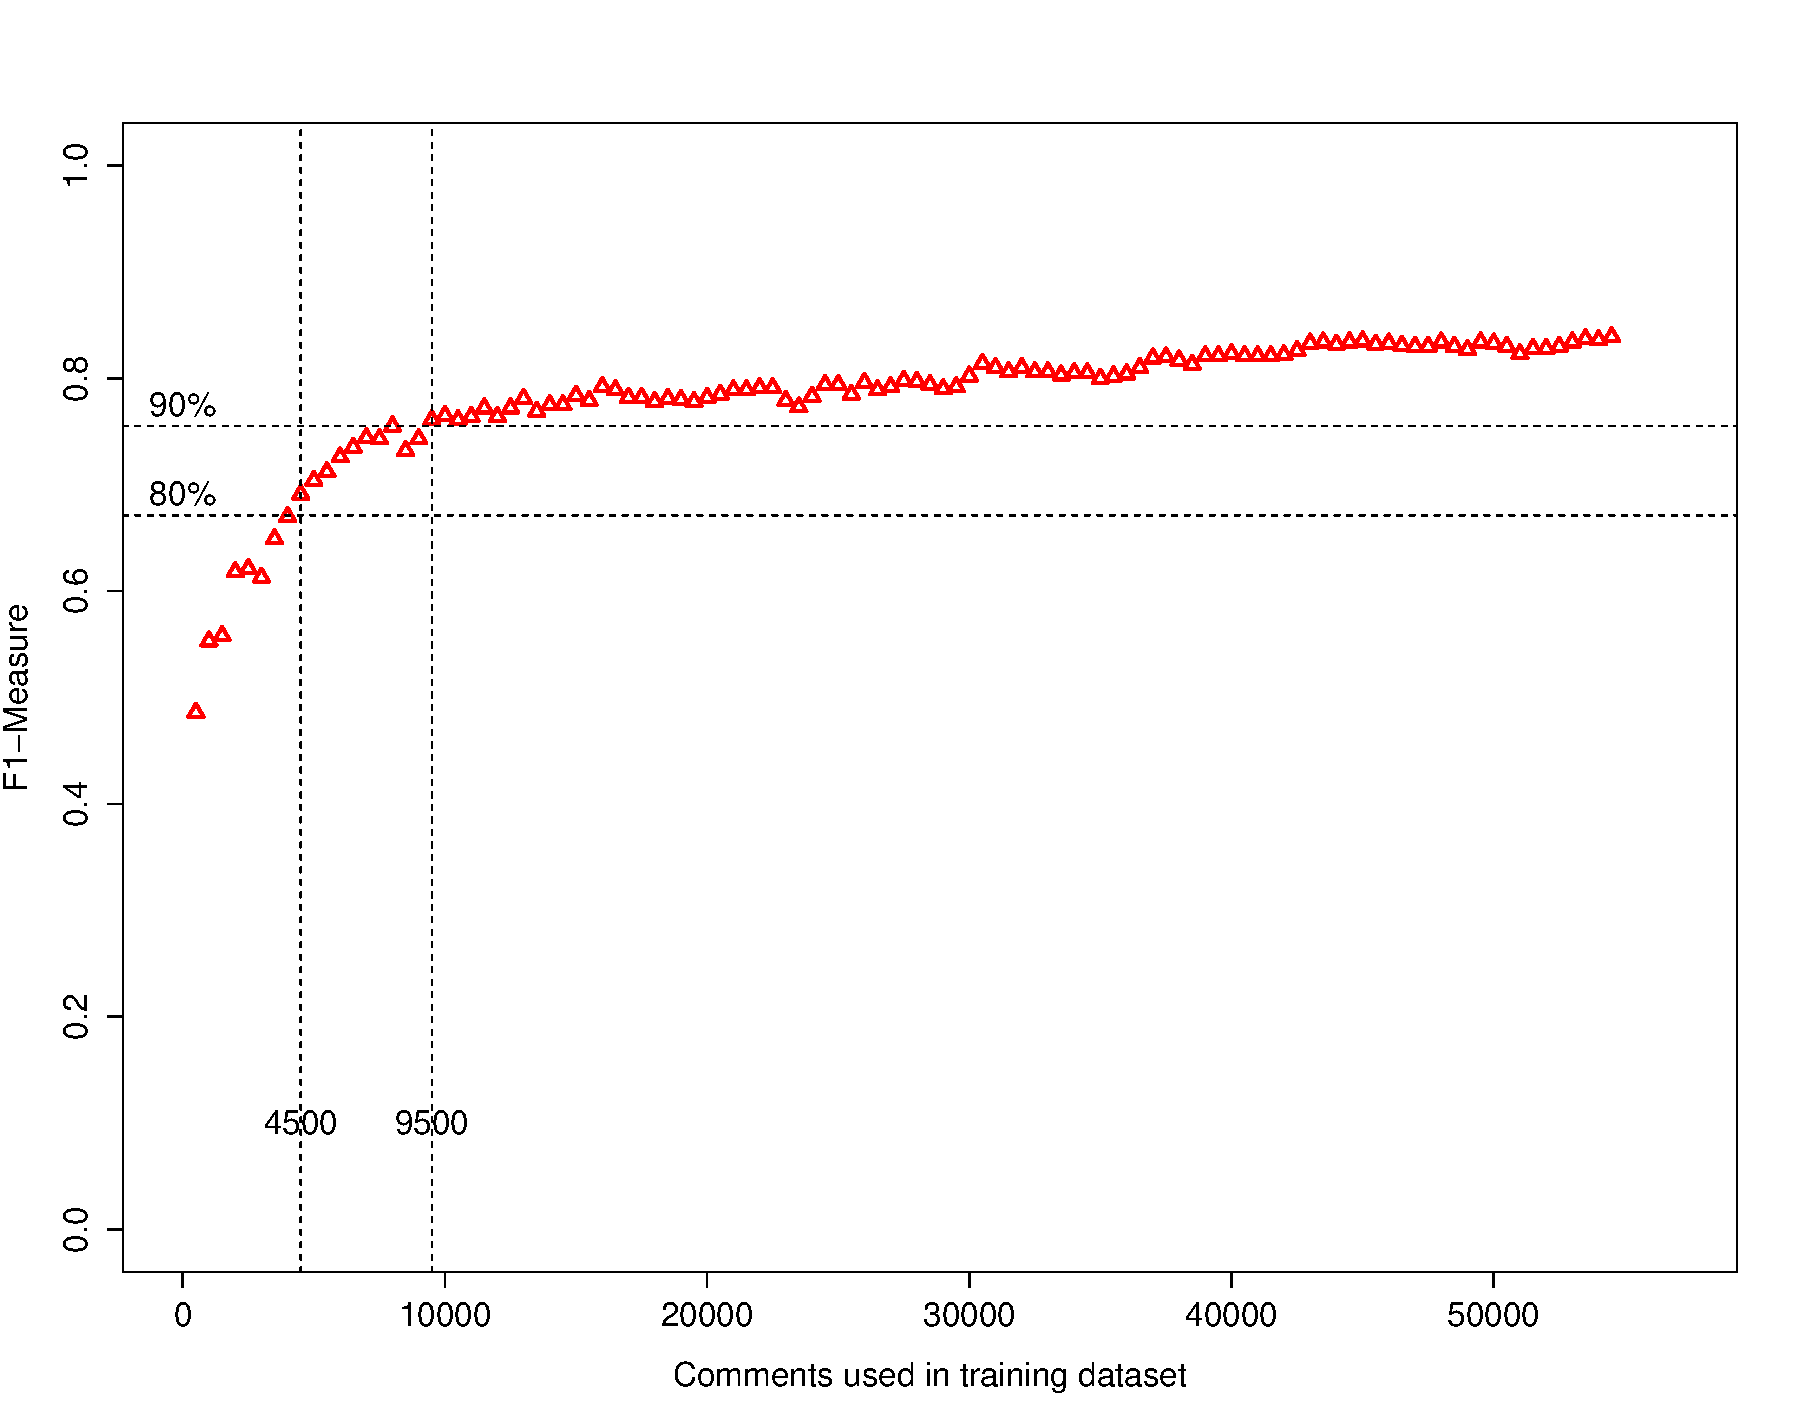
\includegraphics[width=0.49\textwidth]{figures/appendix/ten_fold_validation_design/ten_fold_validation_2_500.pdf}
  \vspace{-5mm}
  \caption{Ten Fold Validation Adding 500 Comments Per Time. Third Iteration}
  \label{fig:design_ten_fold_validation_2_100}
  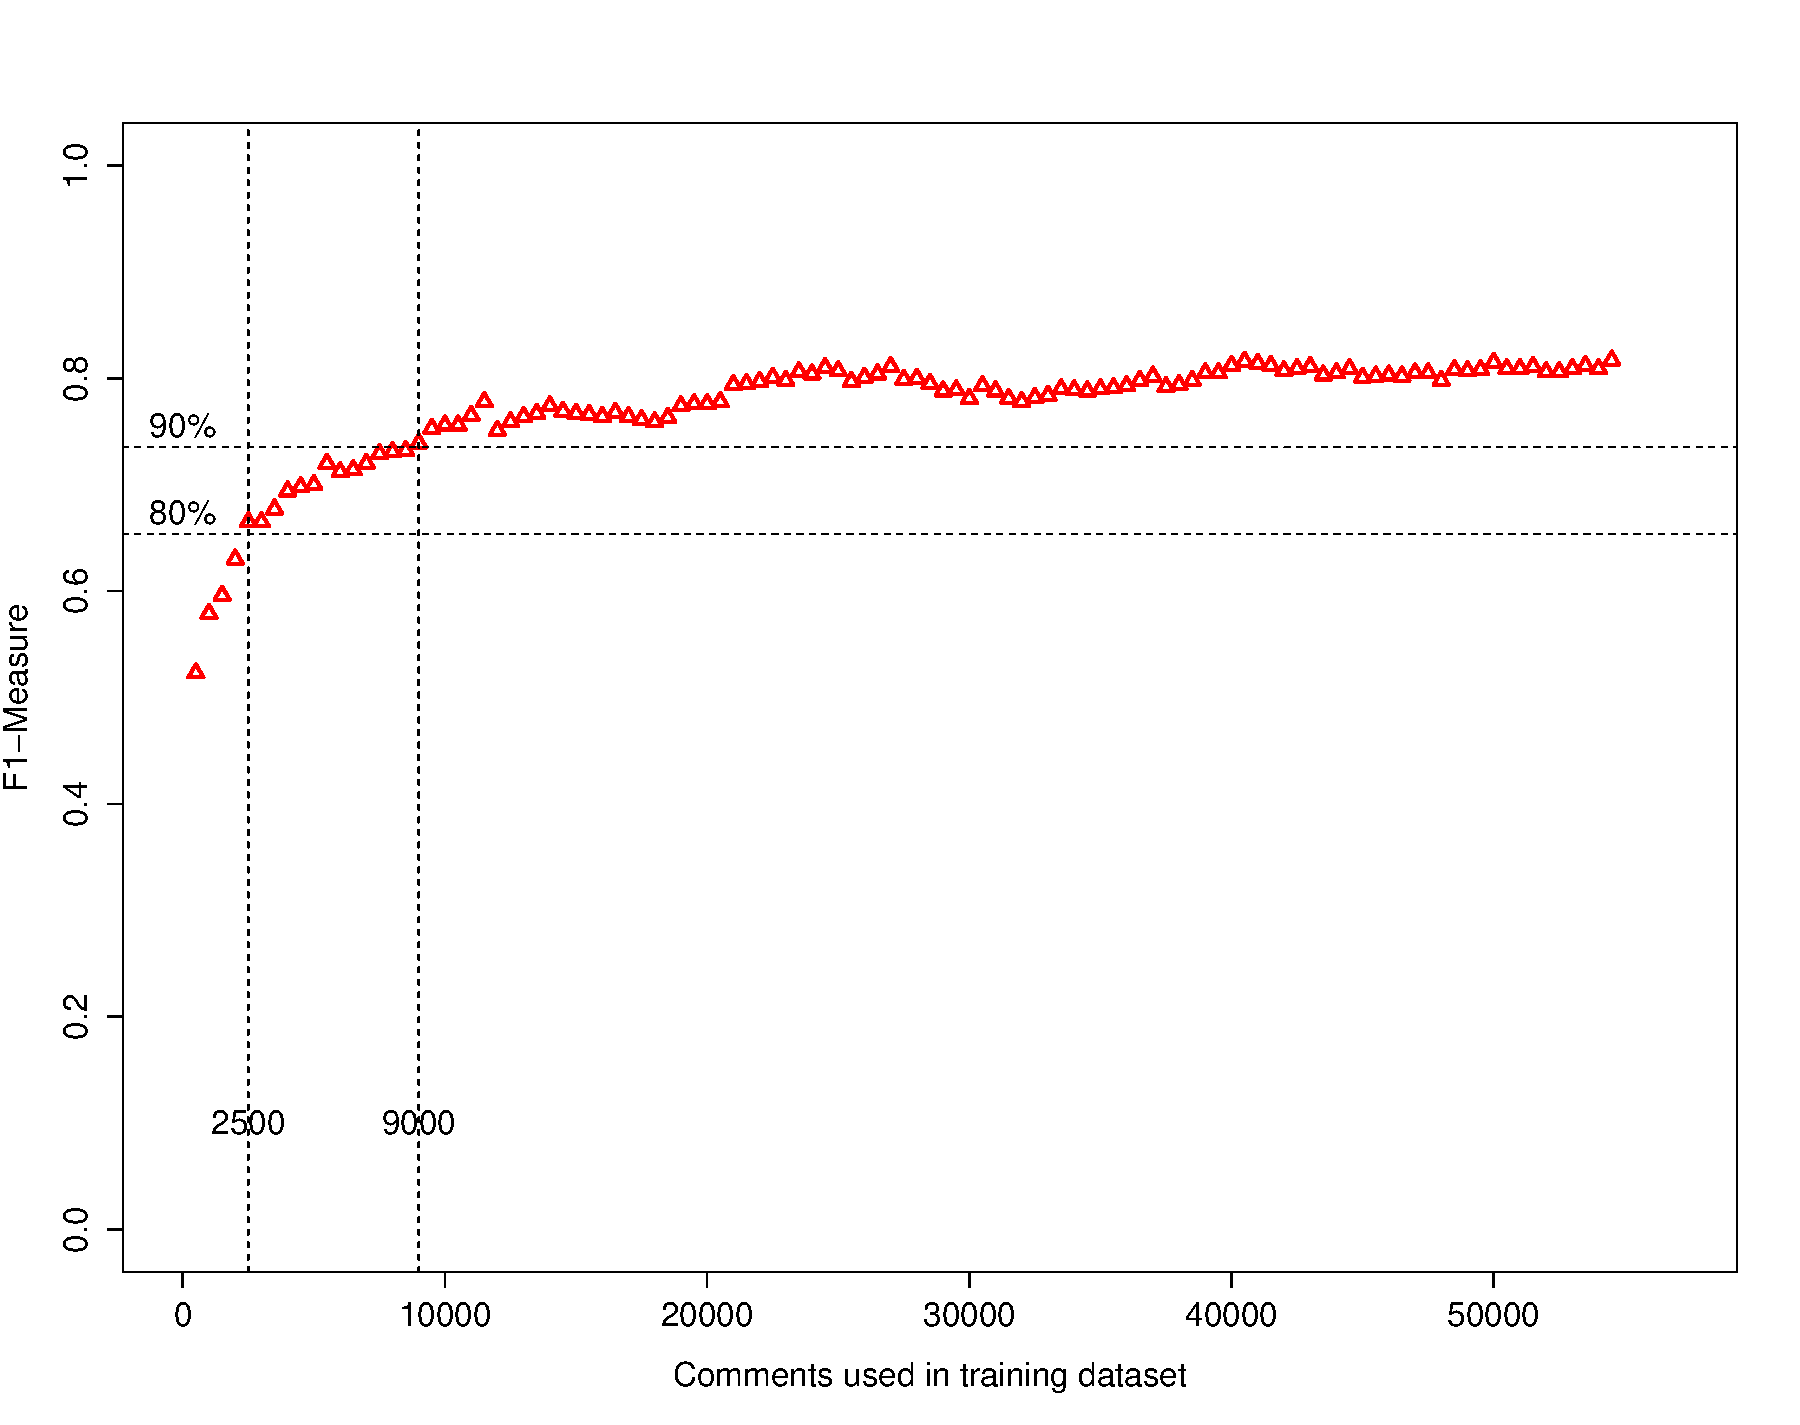
\includegraphics[width=0.49\textwidth]{figures/appendix/ten_fold_validation_design/ten_fold_validation_4_500.pdf}
  \vspace{-5mm}
  \caption{Ten Fold Validation Adding 500 Comments Per Time. Fifth Iteration}
  \label{fig:design_ten_fold_validation_4_100}
\end{figure}

\begin{figure}[thb!]
  \centering
  \vspace{-14mm}
  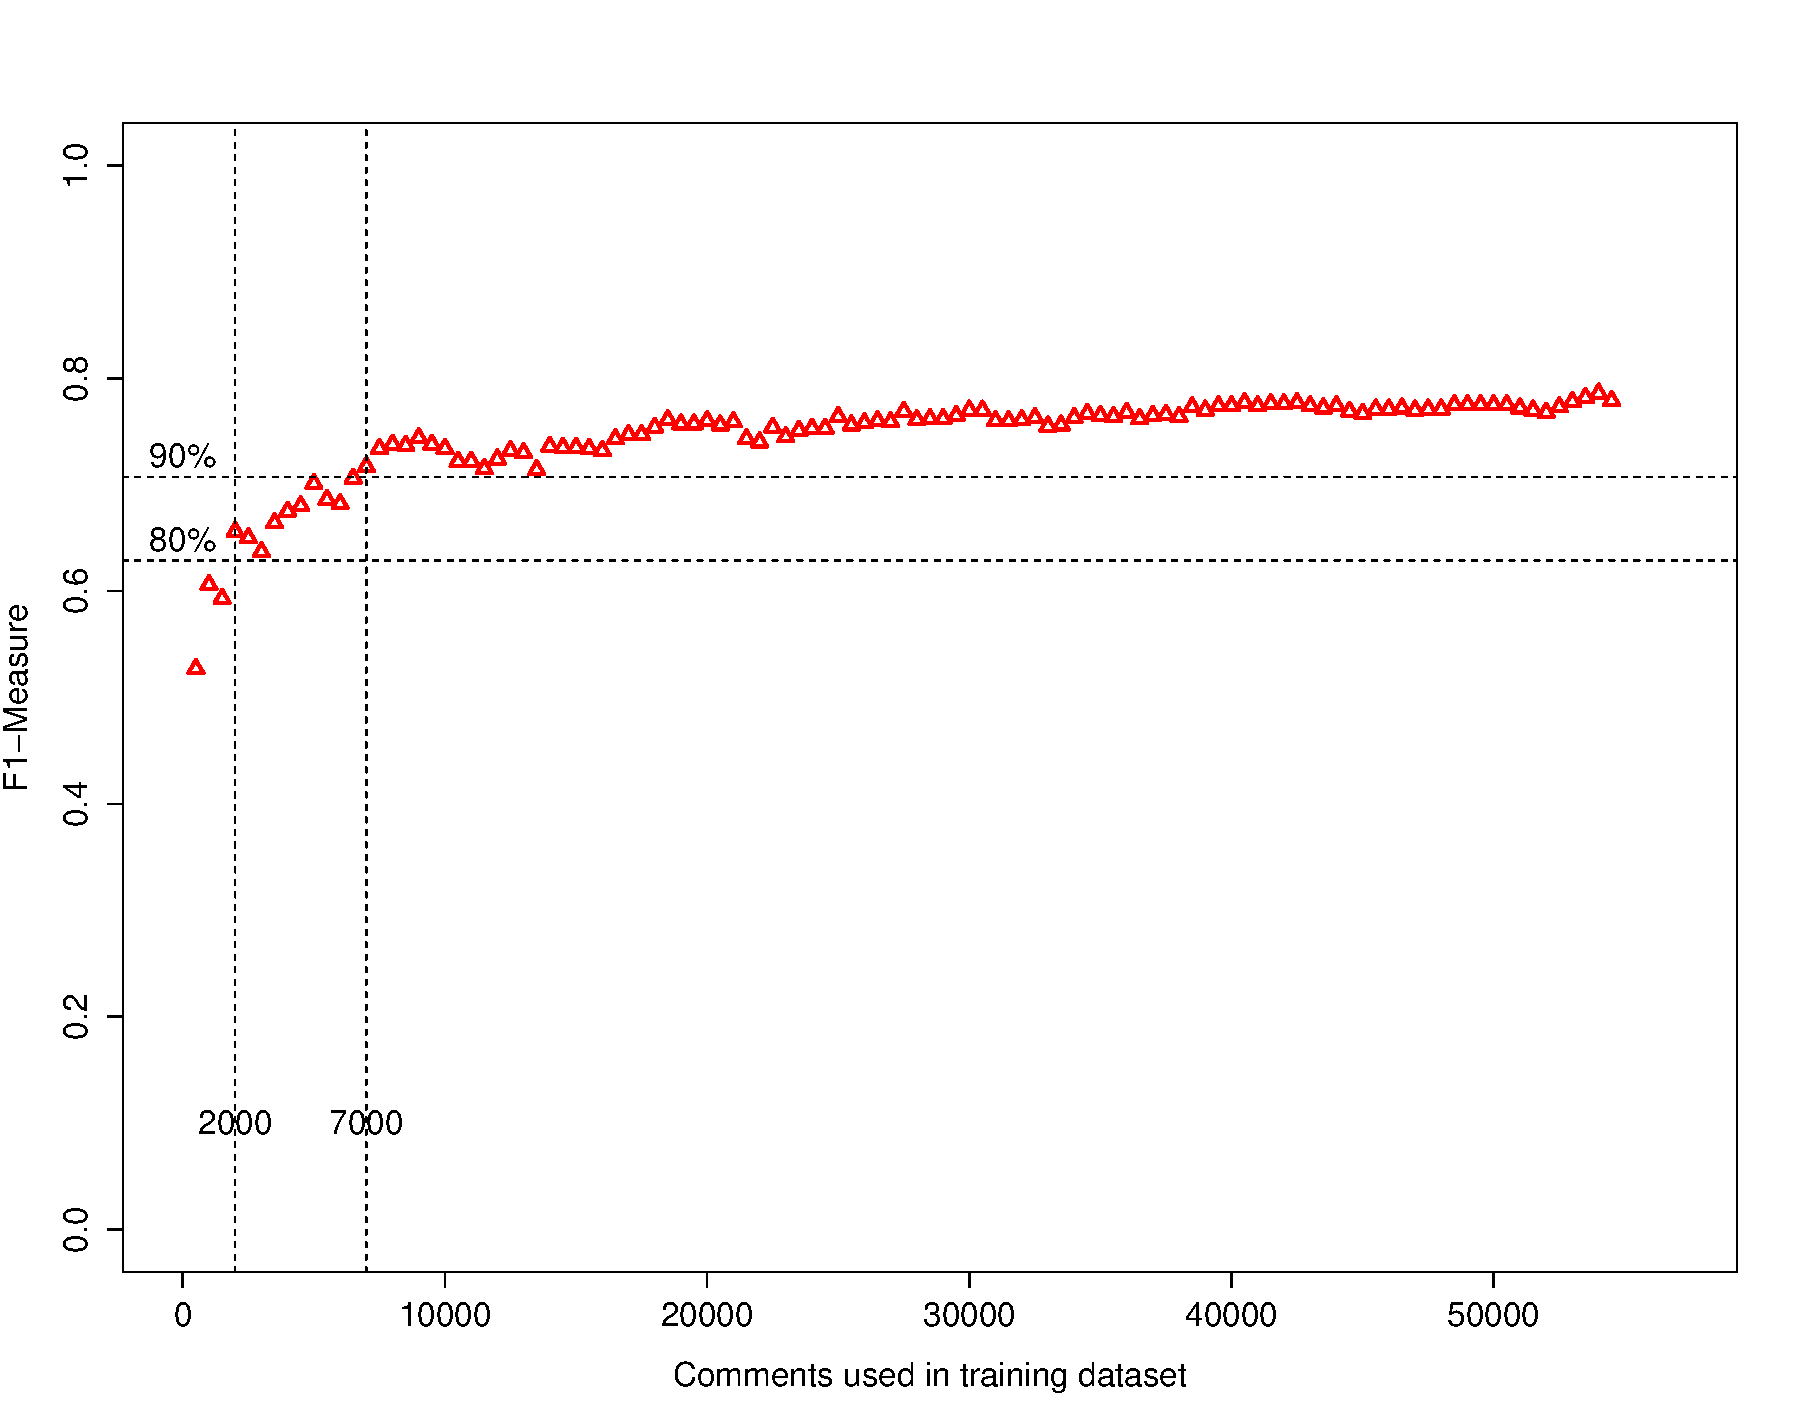
\includegraphics[width=0.49\textwidth]{figures/appendix/ten_fold_validation_design/ten_fold_validation_1_500.pdf}
  \vspace{-5mm}
  \caption{Ten Fold Validation Adding 500 Comments Per Time. Second Iteration}
  \label{fig:design_ten_fold_validation_1_100}
  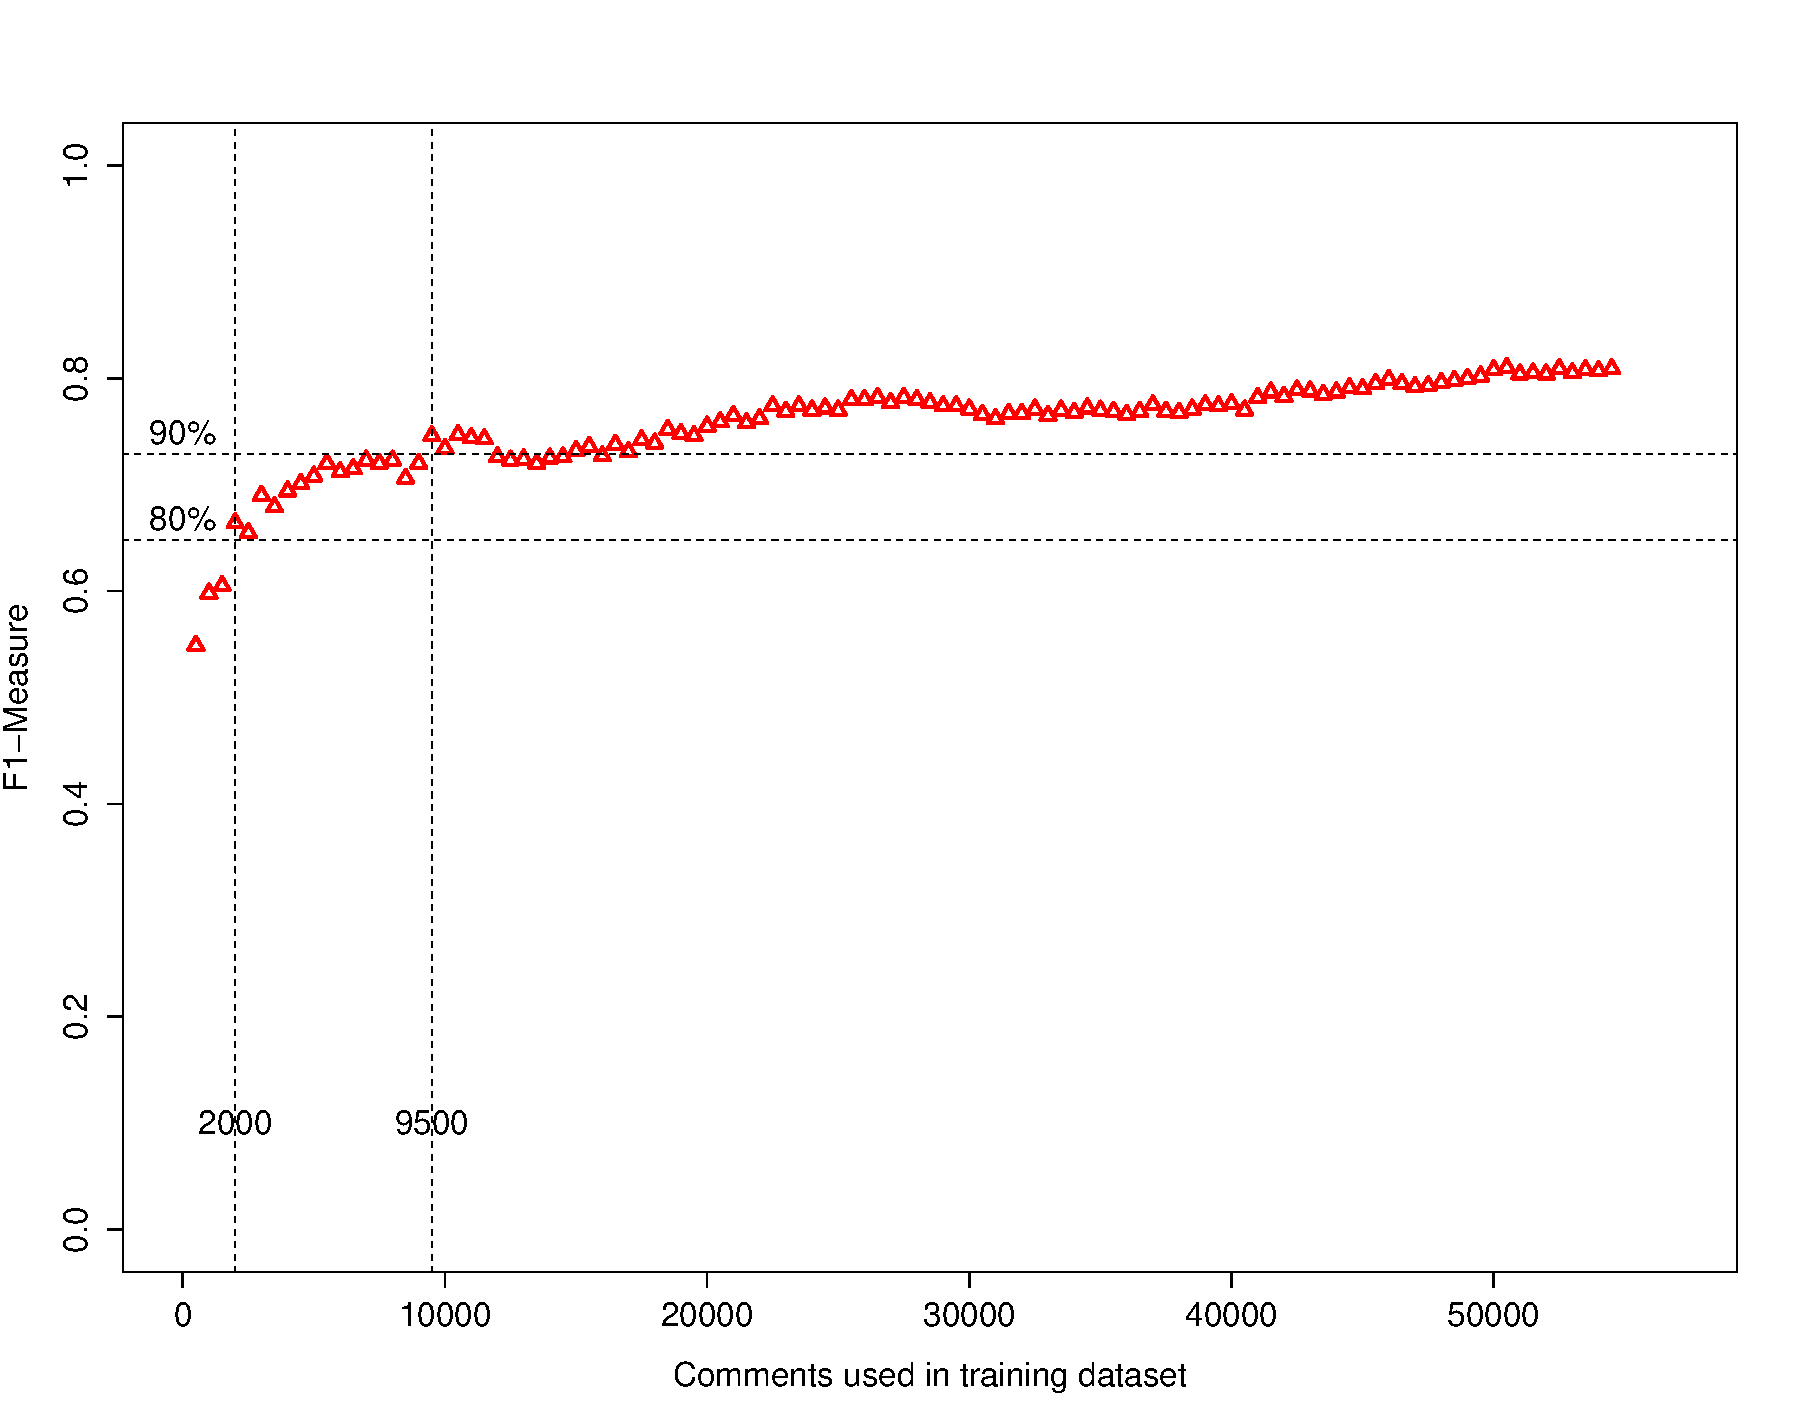
\includegraphics[width=0.49\textwidth]{figures/appendix/ten_fold_validation_design/ten_fold_validation_3_500.pdf}
  \vspace{-5mm}
  \caption{Ten Fold Validation Adding 500 Comments Per Time. Fourth Iteration}
  \label{fig:design_ten_fold_validation_3_100}
  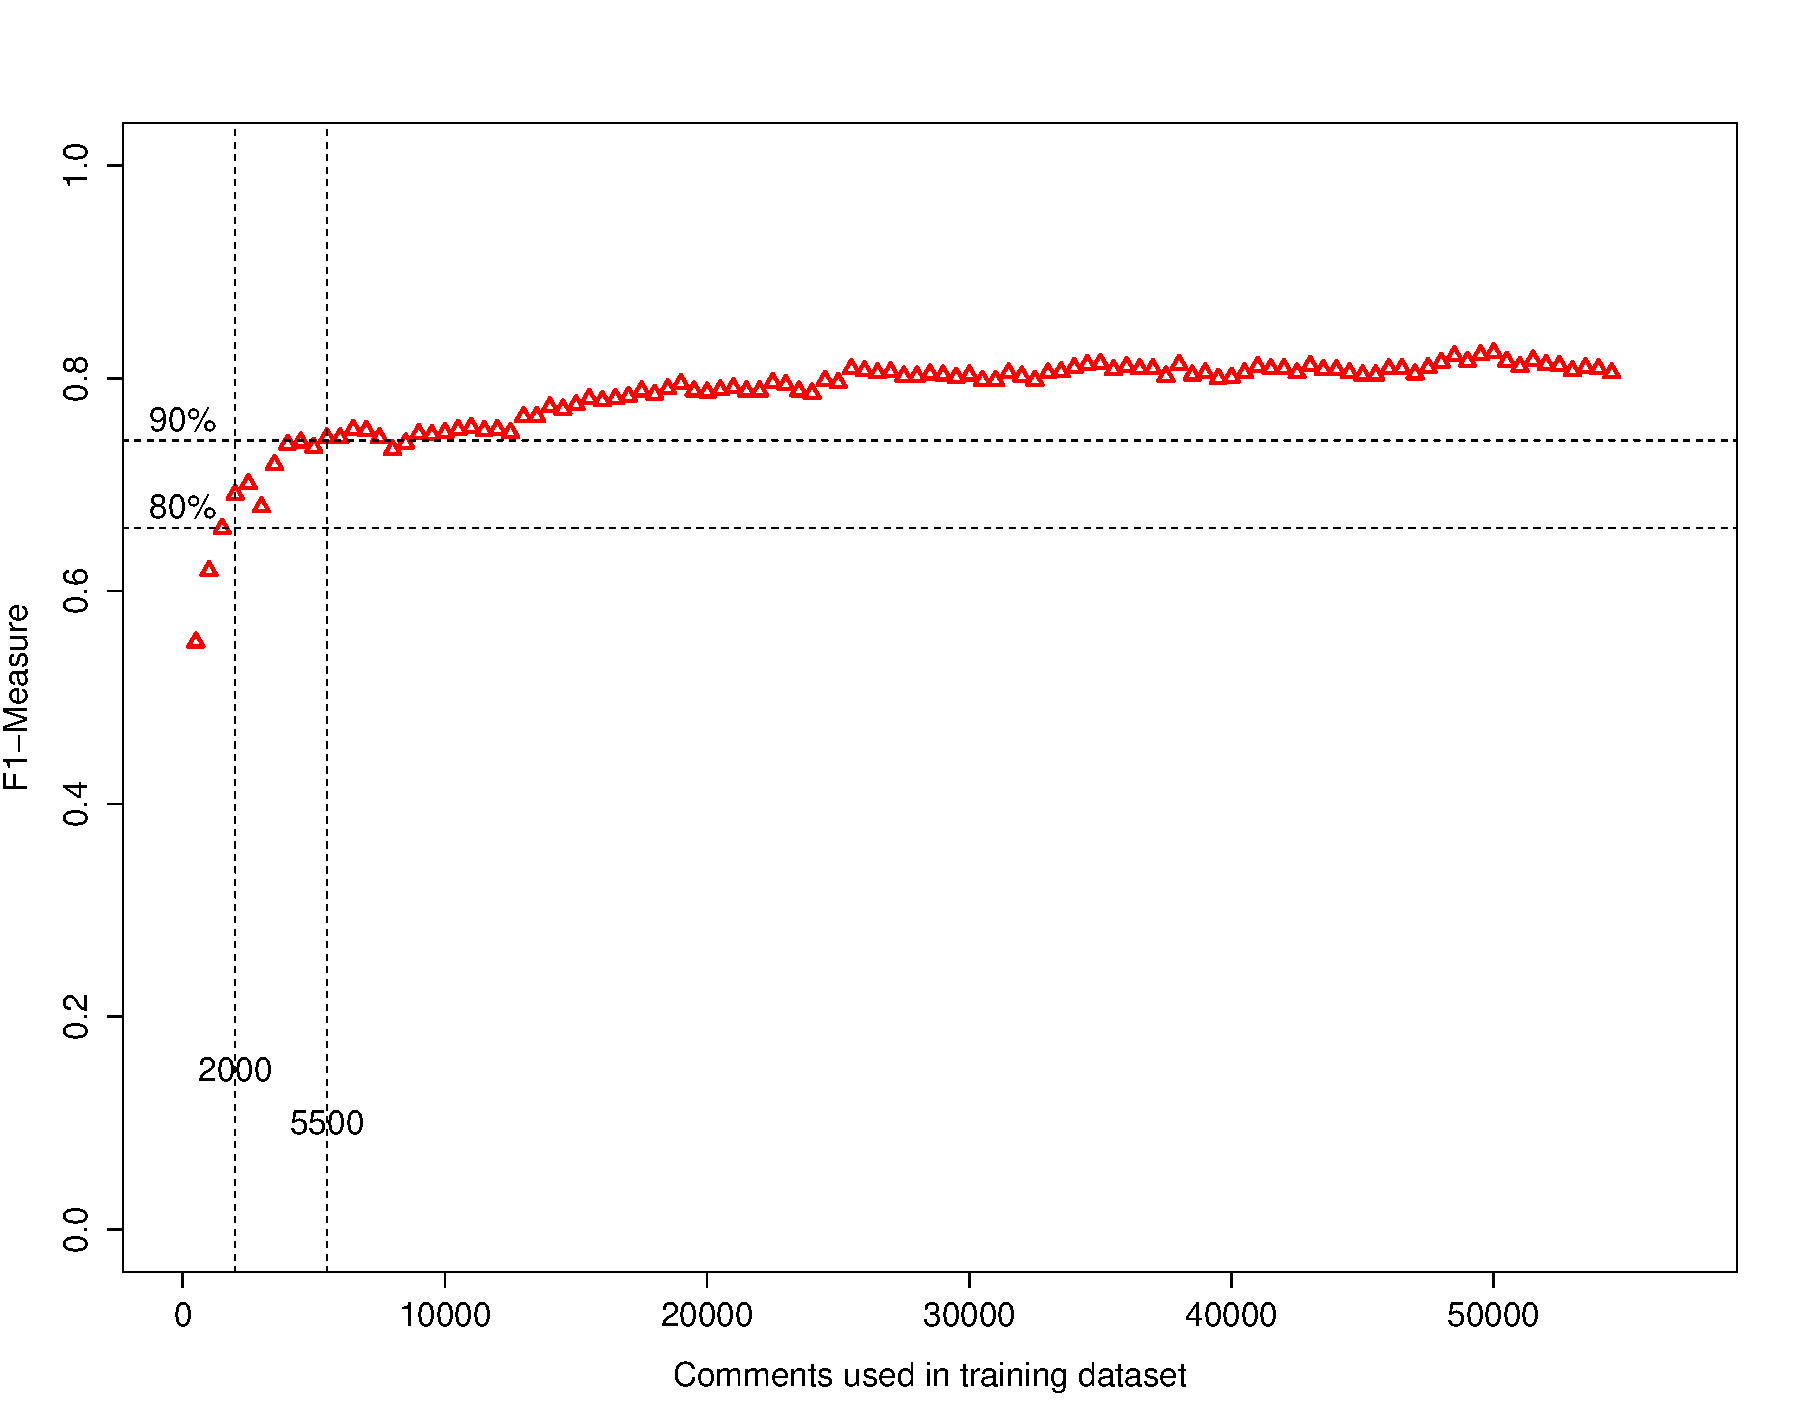
\includegraphics[width=0.49\textwidth]{figures/appendix/ten_fold_validation_design/ten_fold_validation_5_500.pdf}
  \vspace{-5mm}
  \caption{Ten Fold Validation Adding 500 Comments Per Time. Sixth Iteration}
  \label{fig:design_ten_fold_validation_5_100}
\end{figure}

\clearpage
\begin{figure}[thb!]
  \centering
  \vspace{-3mm}
  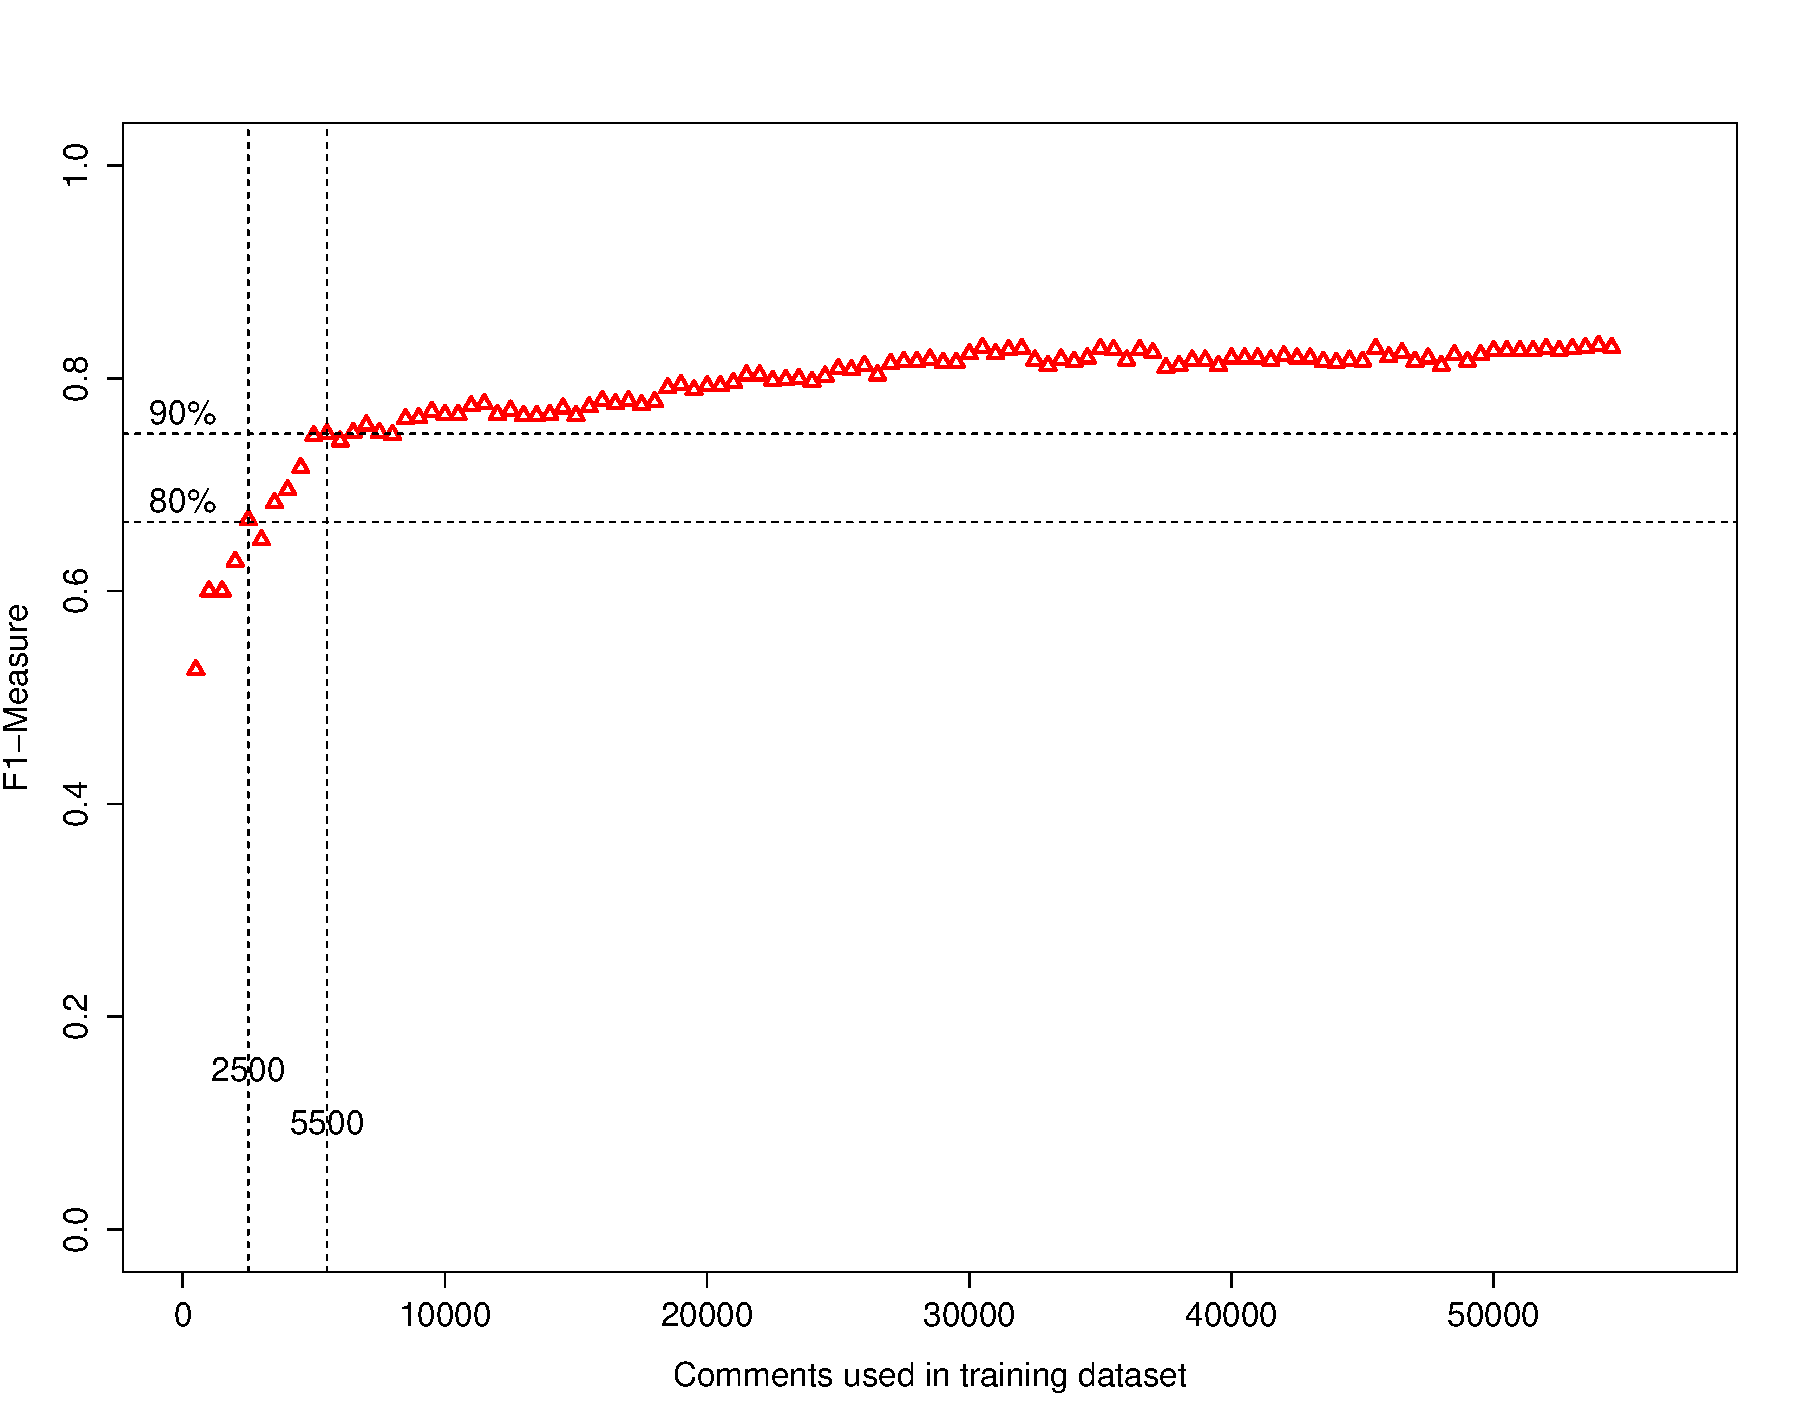
\includegraphics[width=0.49\textwidth]{figures/appendix/ten_fold_validation_design/ten_fold_validation_6_500.pdf}
  \vspace{-5mm}
  \caption{Ten Fold Validation Adding 500 Comments Per Time. Seventh Iteration}
  \label{fig:design_ten_fold_validation_6_100}
  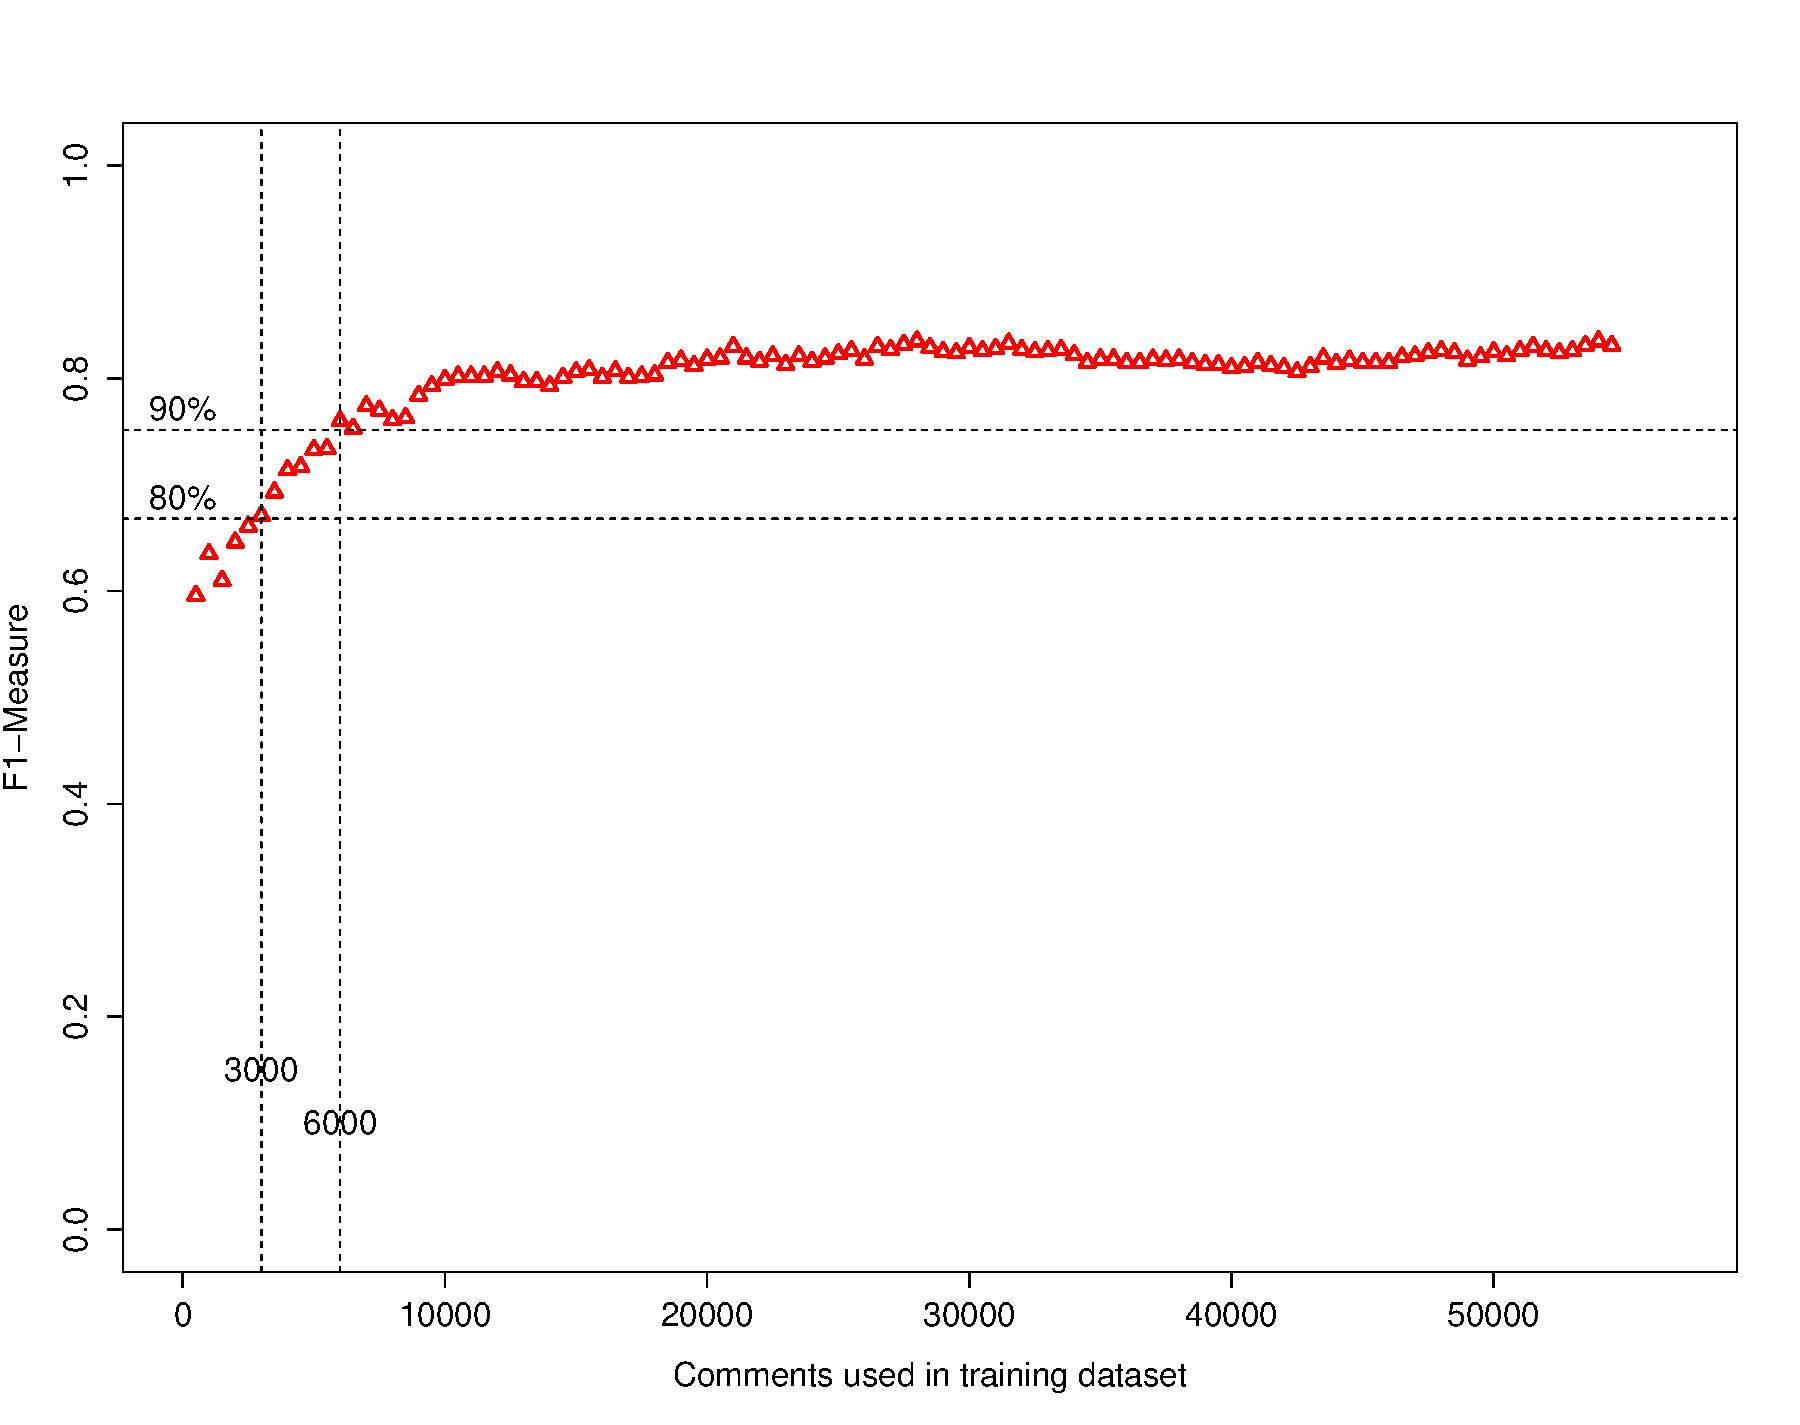
\includegraphics[width=0.49\textwidth]{figures/appendix/ten_fold_validation_design/ten_fold_validation_8_500.pdf}
  \vspace{-5mm}
  \caption{Ten Fold Validation Adding 500 Comments Per Time. Ninth Iteration}
  \label{fig:design_ten_fold_validation_8_100}
  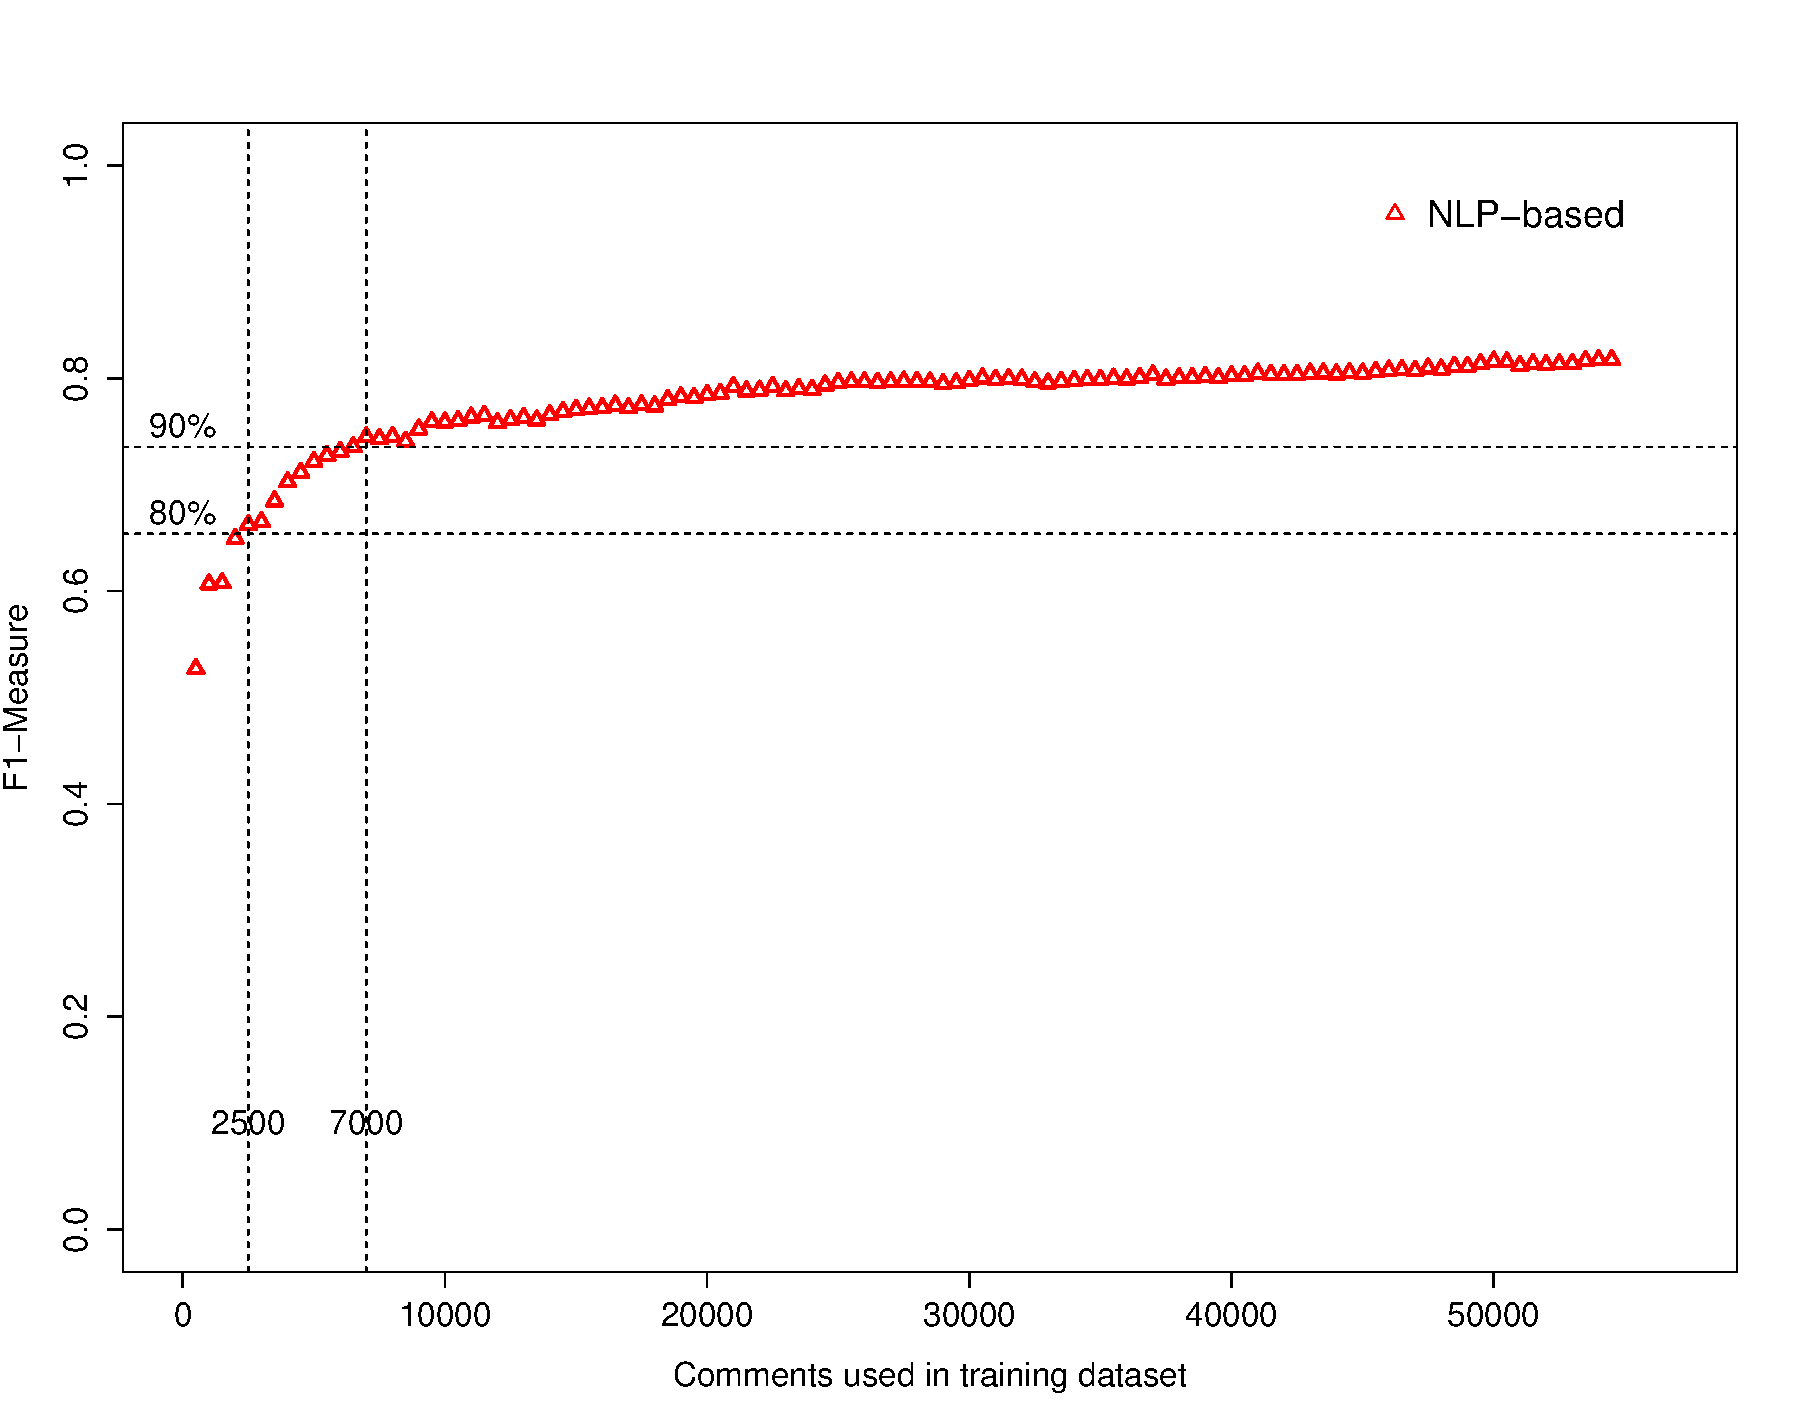
\includegraphics[width=0.49\textwidth]{figures/appendix/ten_fold_validation_design/ten_fold_validation_average_500.pdf}
  \vspace{-5mm}
  \caption{Ten Fold Validation Adding 500 Comments Per Time. Average}
  \label{fig:design_ten_fold_validation_average_100}
\end{figure}

\begin{figure}[thb!]
  \centering
  \vspace{-93mm}
  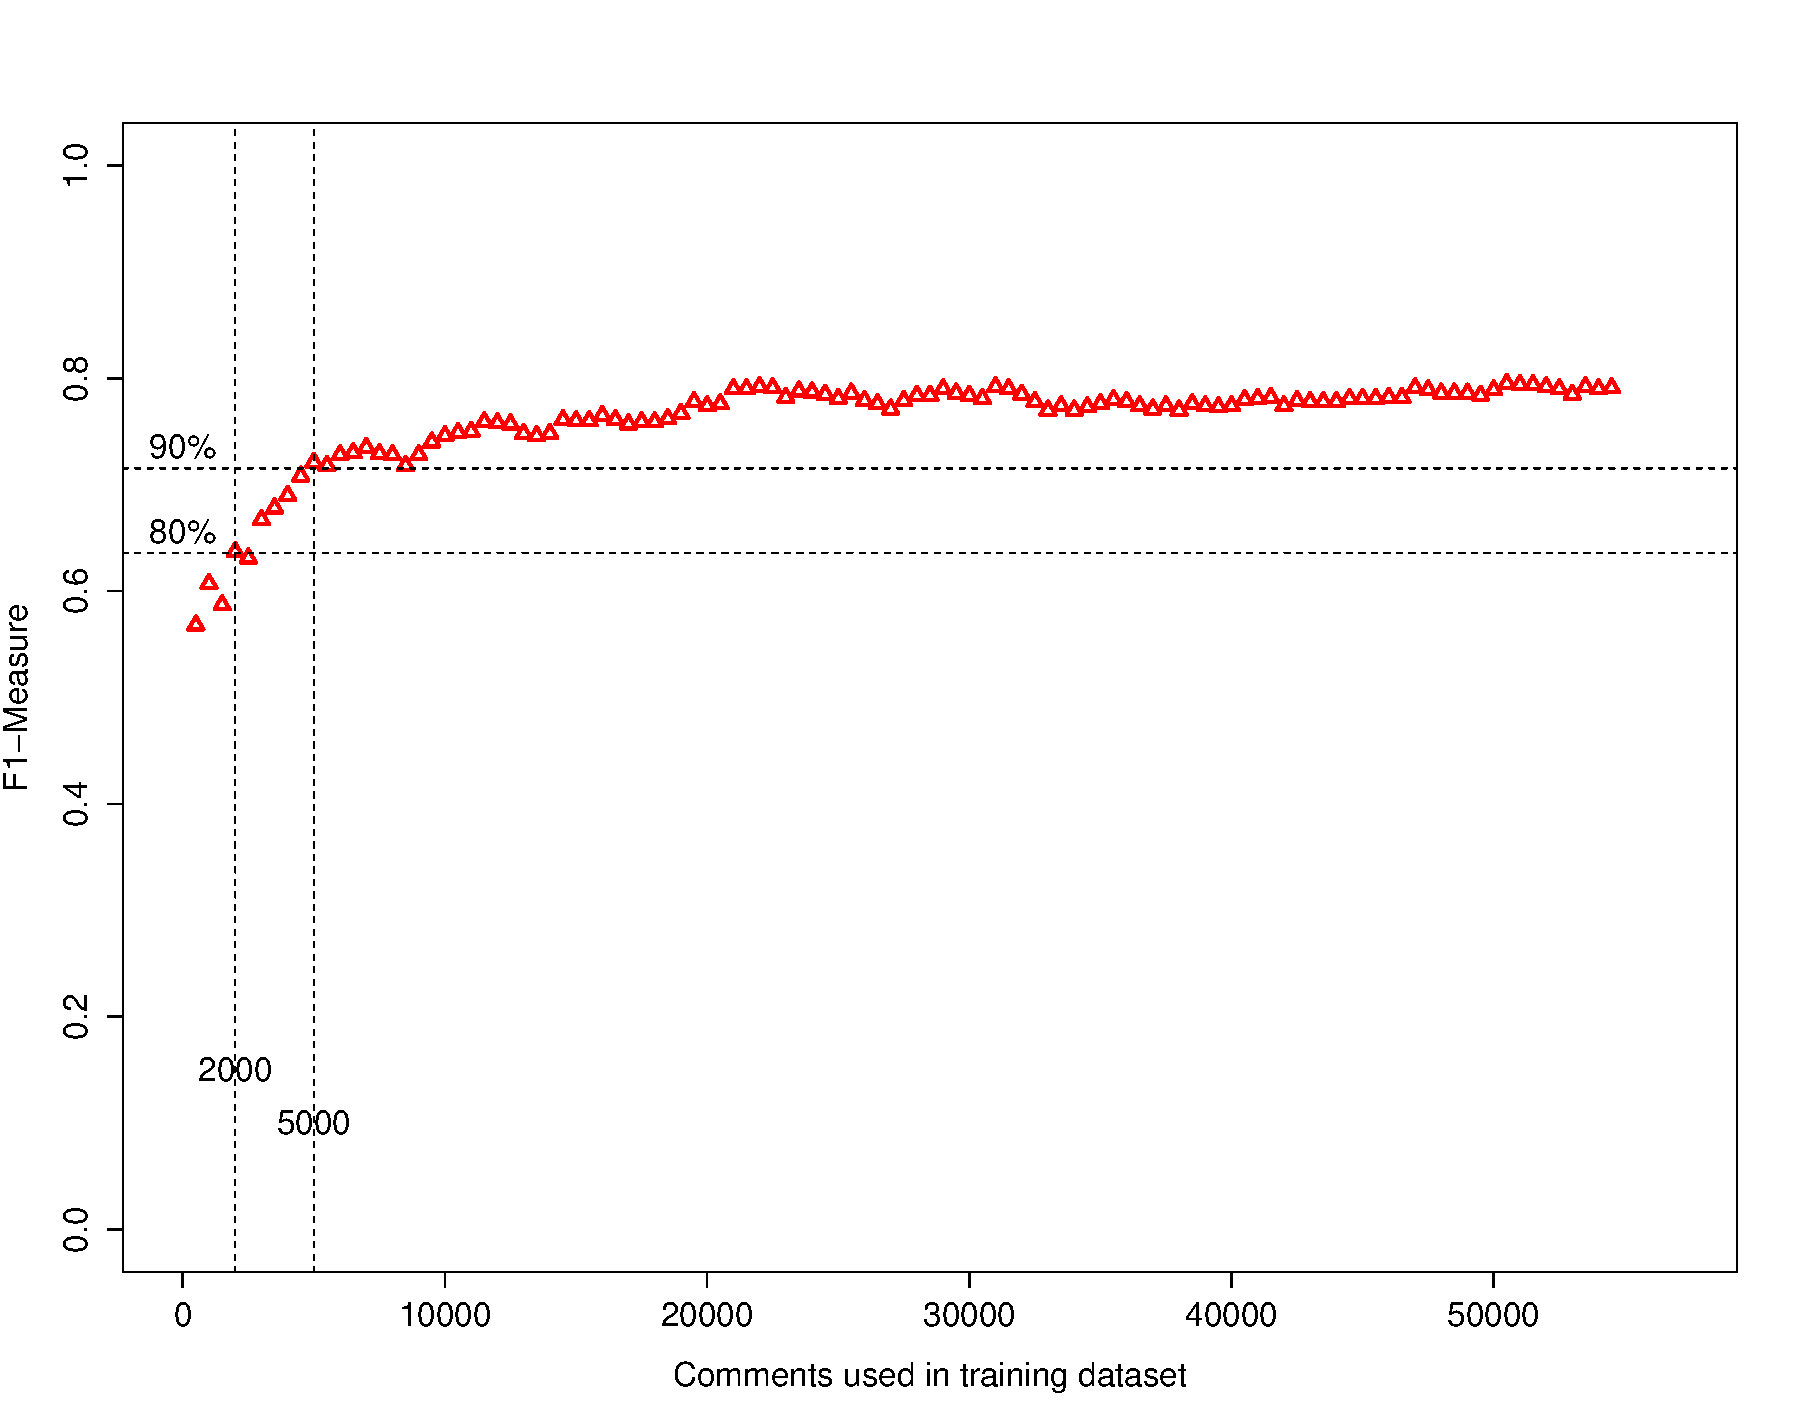
\includegraphics[width=0.49\textwidth]{figures/appendix/ten_fold_validation_design/ten_fold_validation_7_500.pdf}
  \vspace{-5mm}
  \caption{Ten Fold Validation Adding 500 Comments Per Time. Eight Iteration}
  \label{fig:design_ten_fold_validation_7_100}
  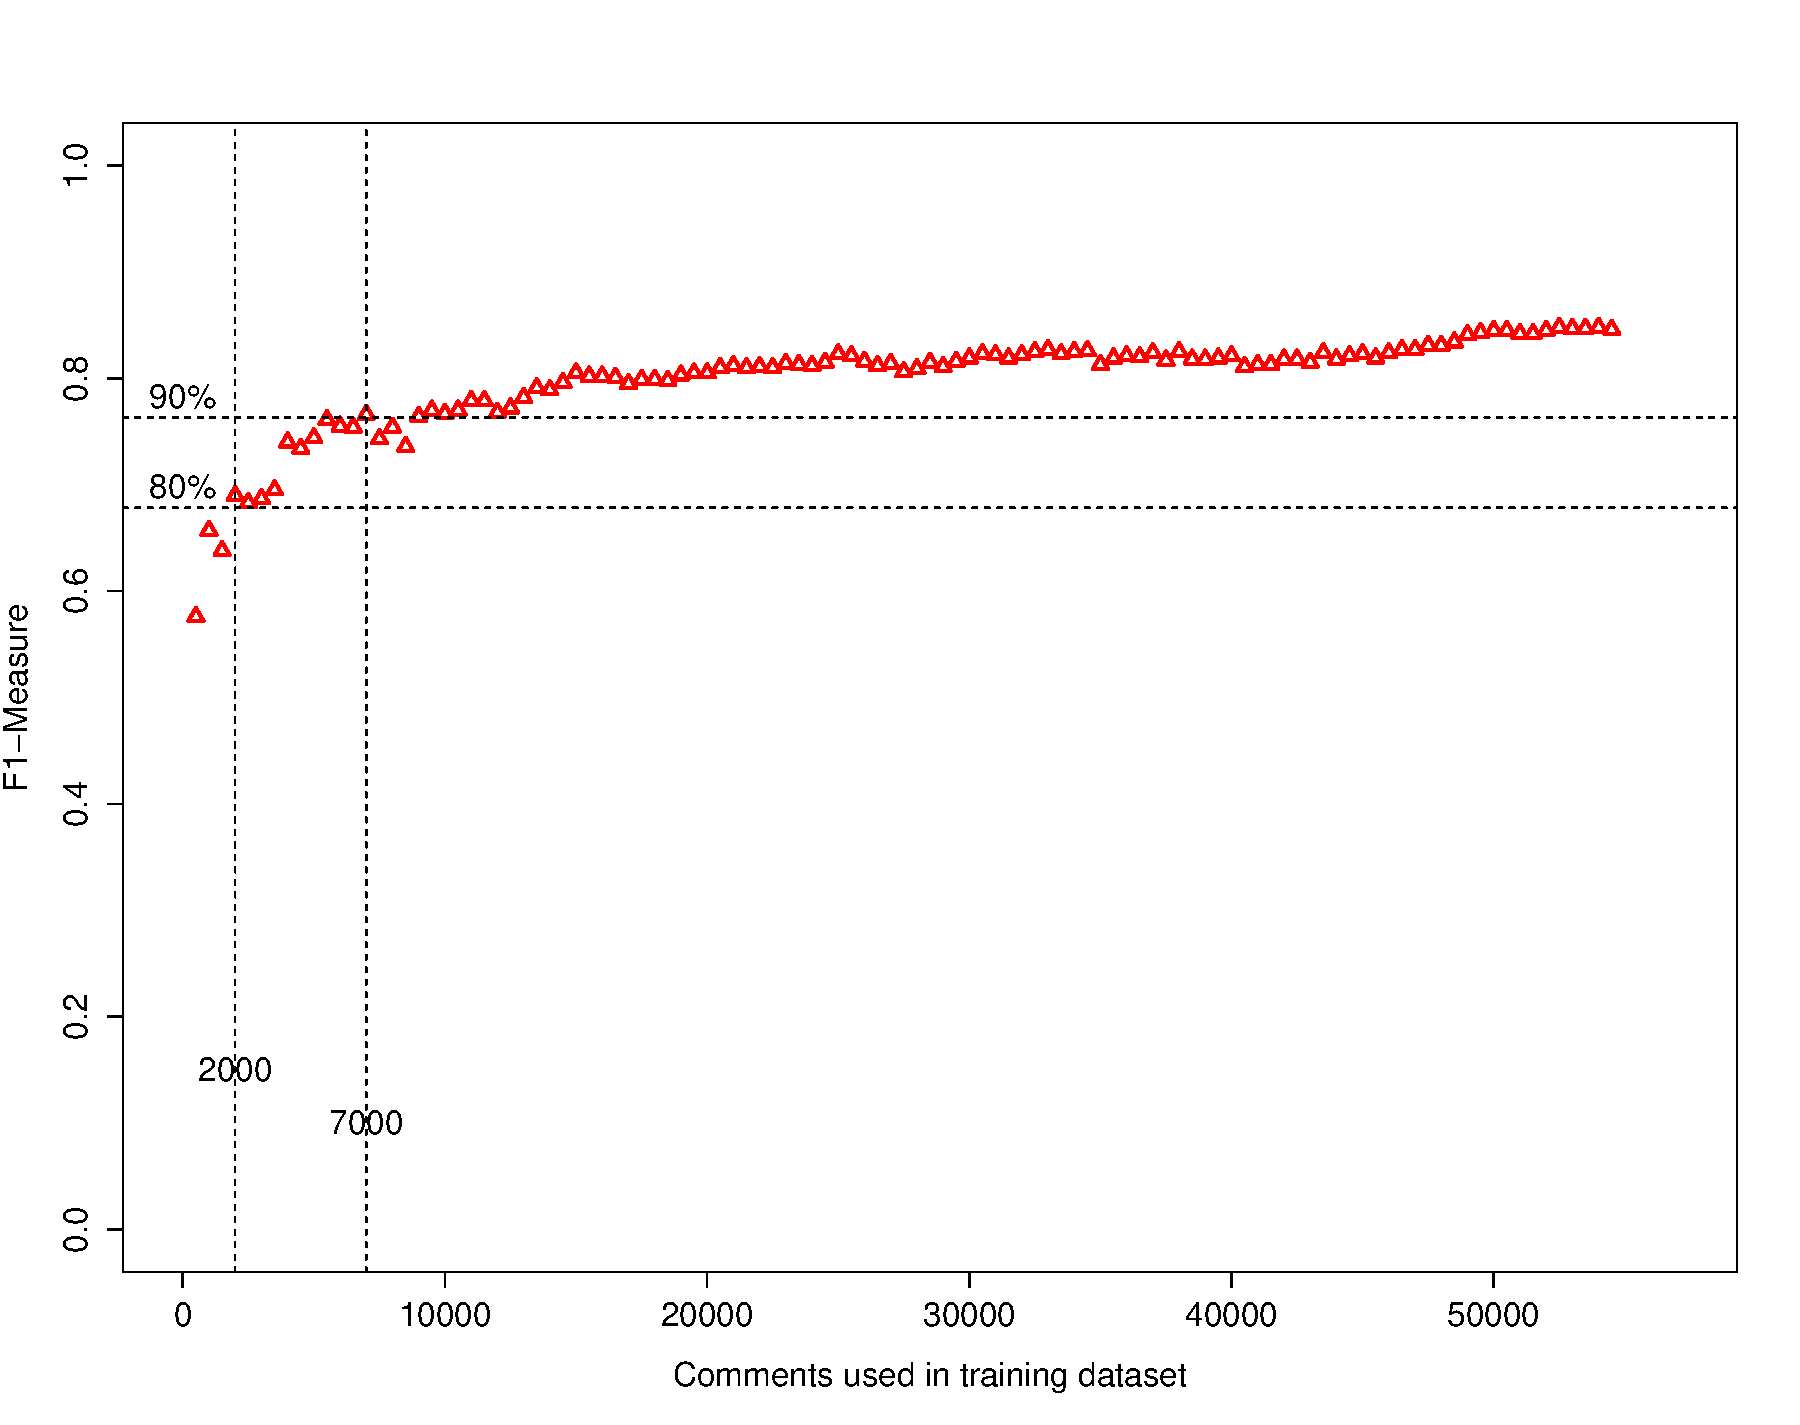
\includegraphics[width=0.49\textwidth]{figures/appendix/ten_fold_validation_design/ten_fold_validation_9_500.pdf}
  \vspace{-5mm}
  \caption{Ten Fold Validation Adding 500 Comments Per Time. Tenth Iteration}
  \label{fig:design_ten_fold_validation_9_100}
  
\end{figure}

% ------------------------------------

\clearpage
\begin{figure}[thb!]
  \centering
  \vspace{-3mm}
  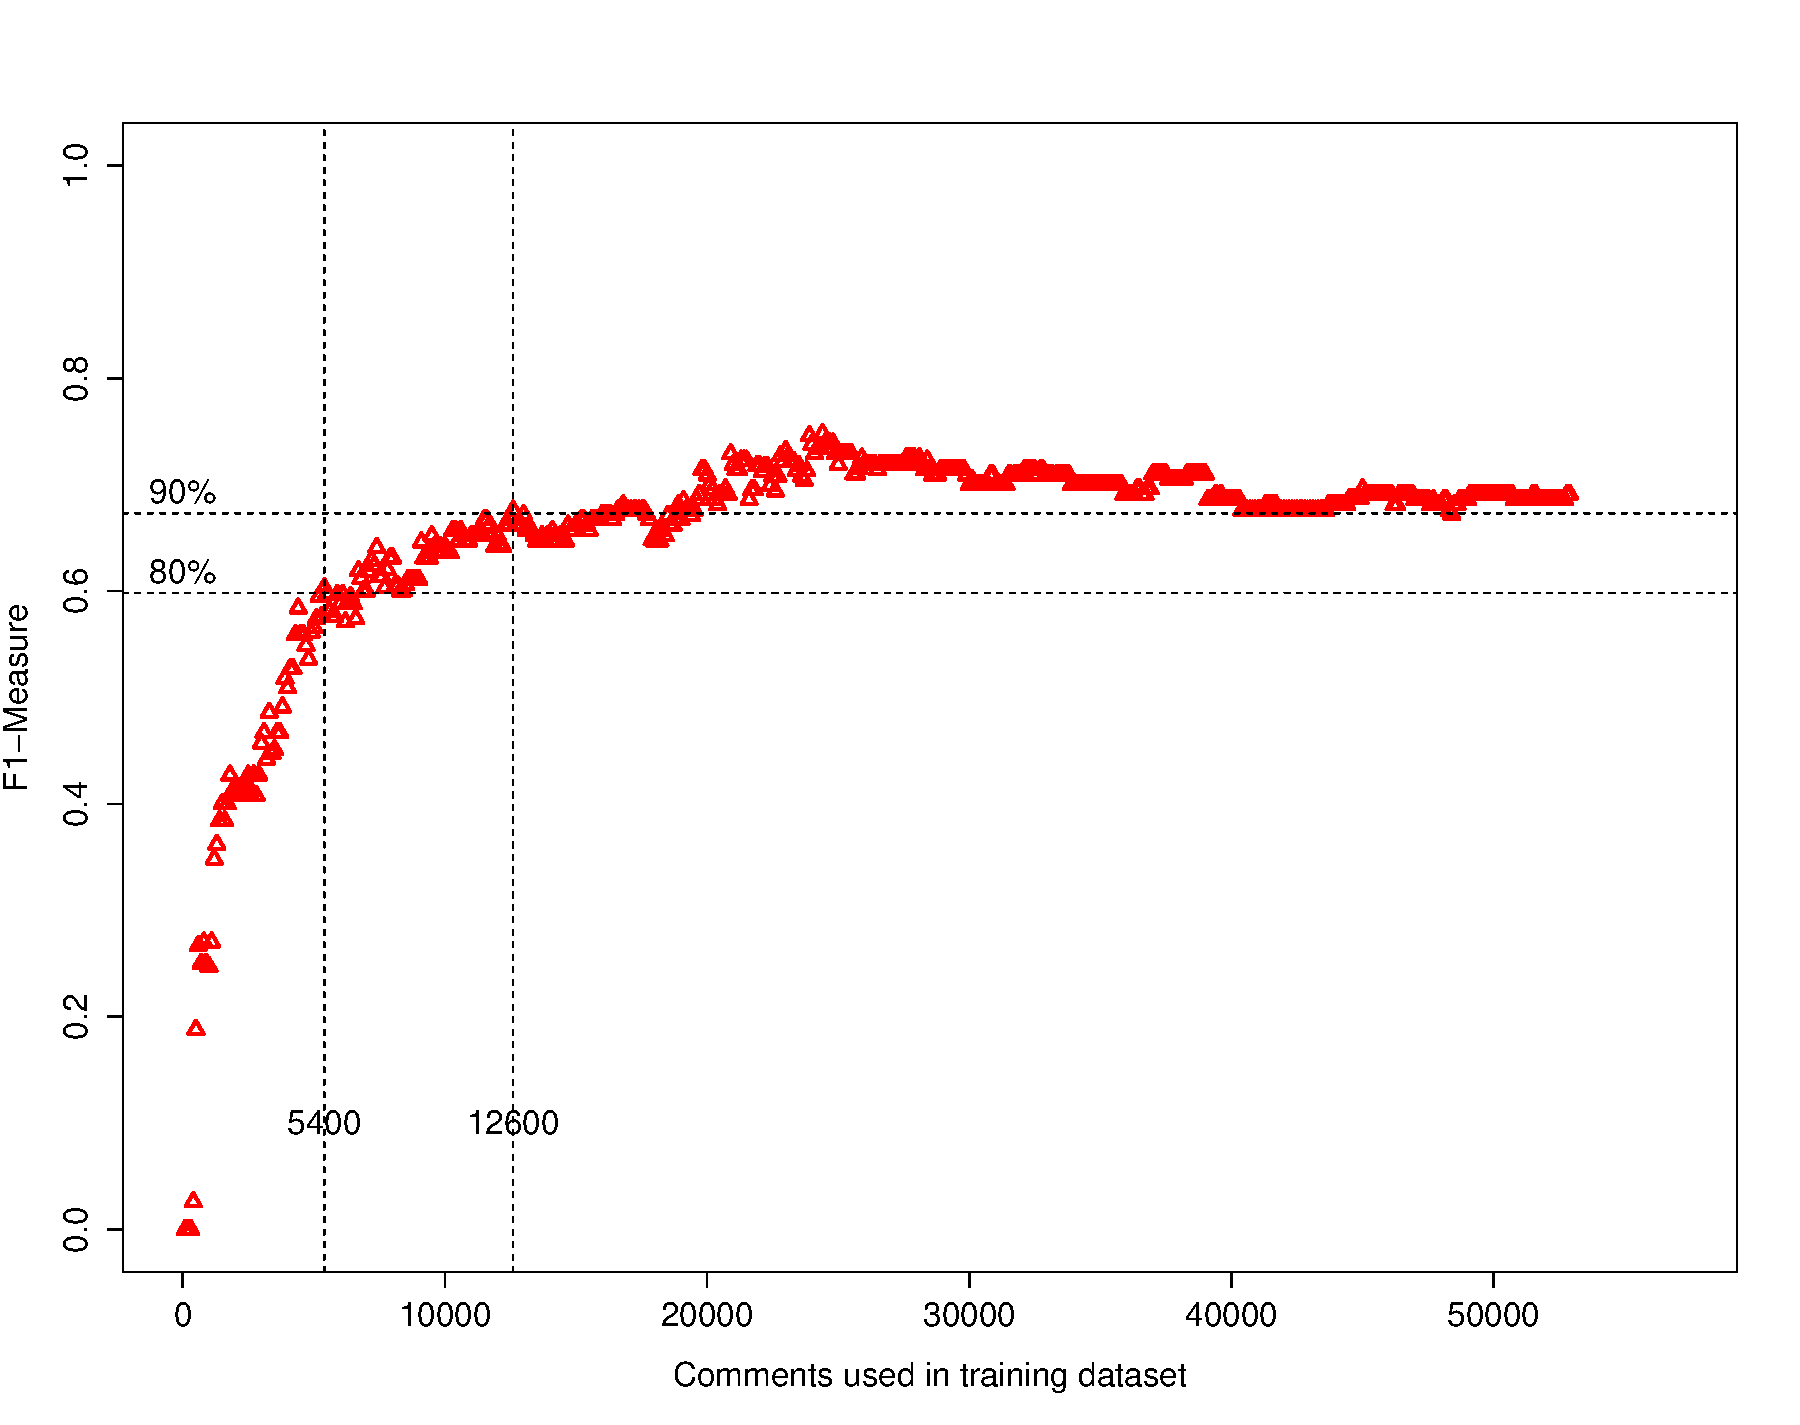
\includegraphics[width=0.49\textwidth]{figures/appendix/ten_fold_validation_requirement/ten_fold_validation_0_100.pdf}
  \vspace{-5mm}
  \caption{Ten Fold Validation Adding 100 Comments Per Time. First Iteration}
  \label{fig:requirement_ten_fold_validation_0_100}
  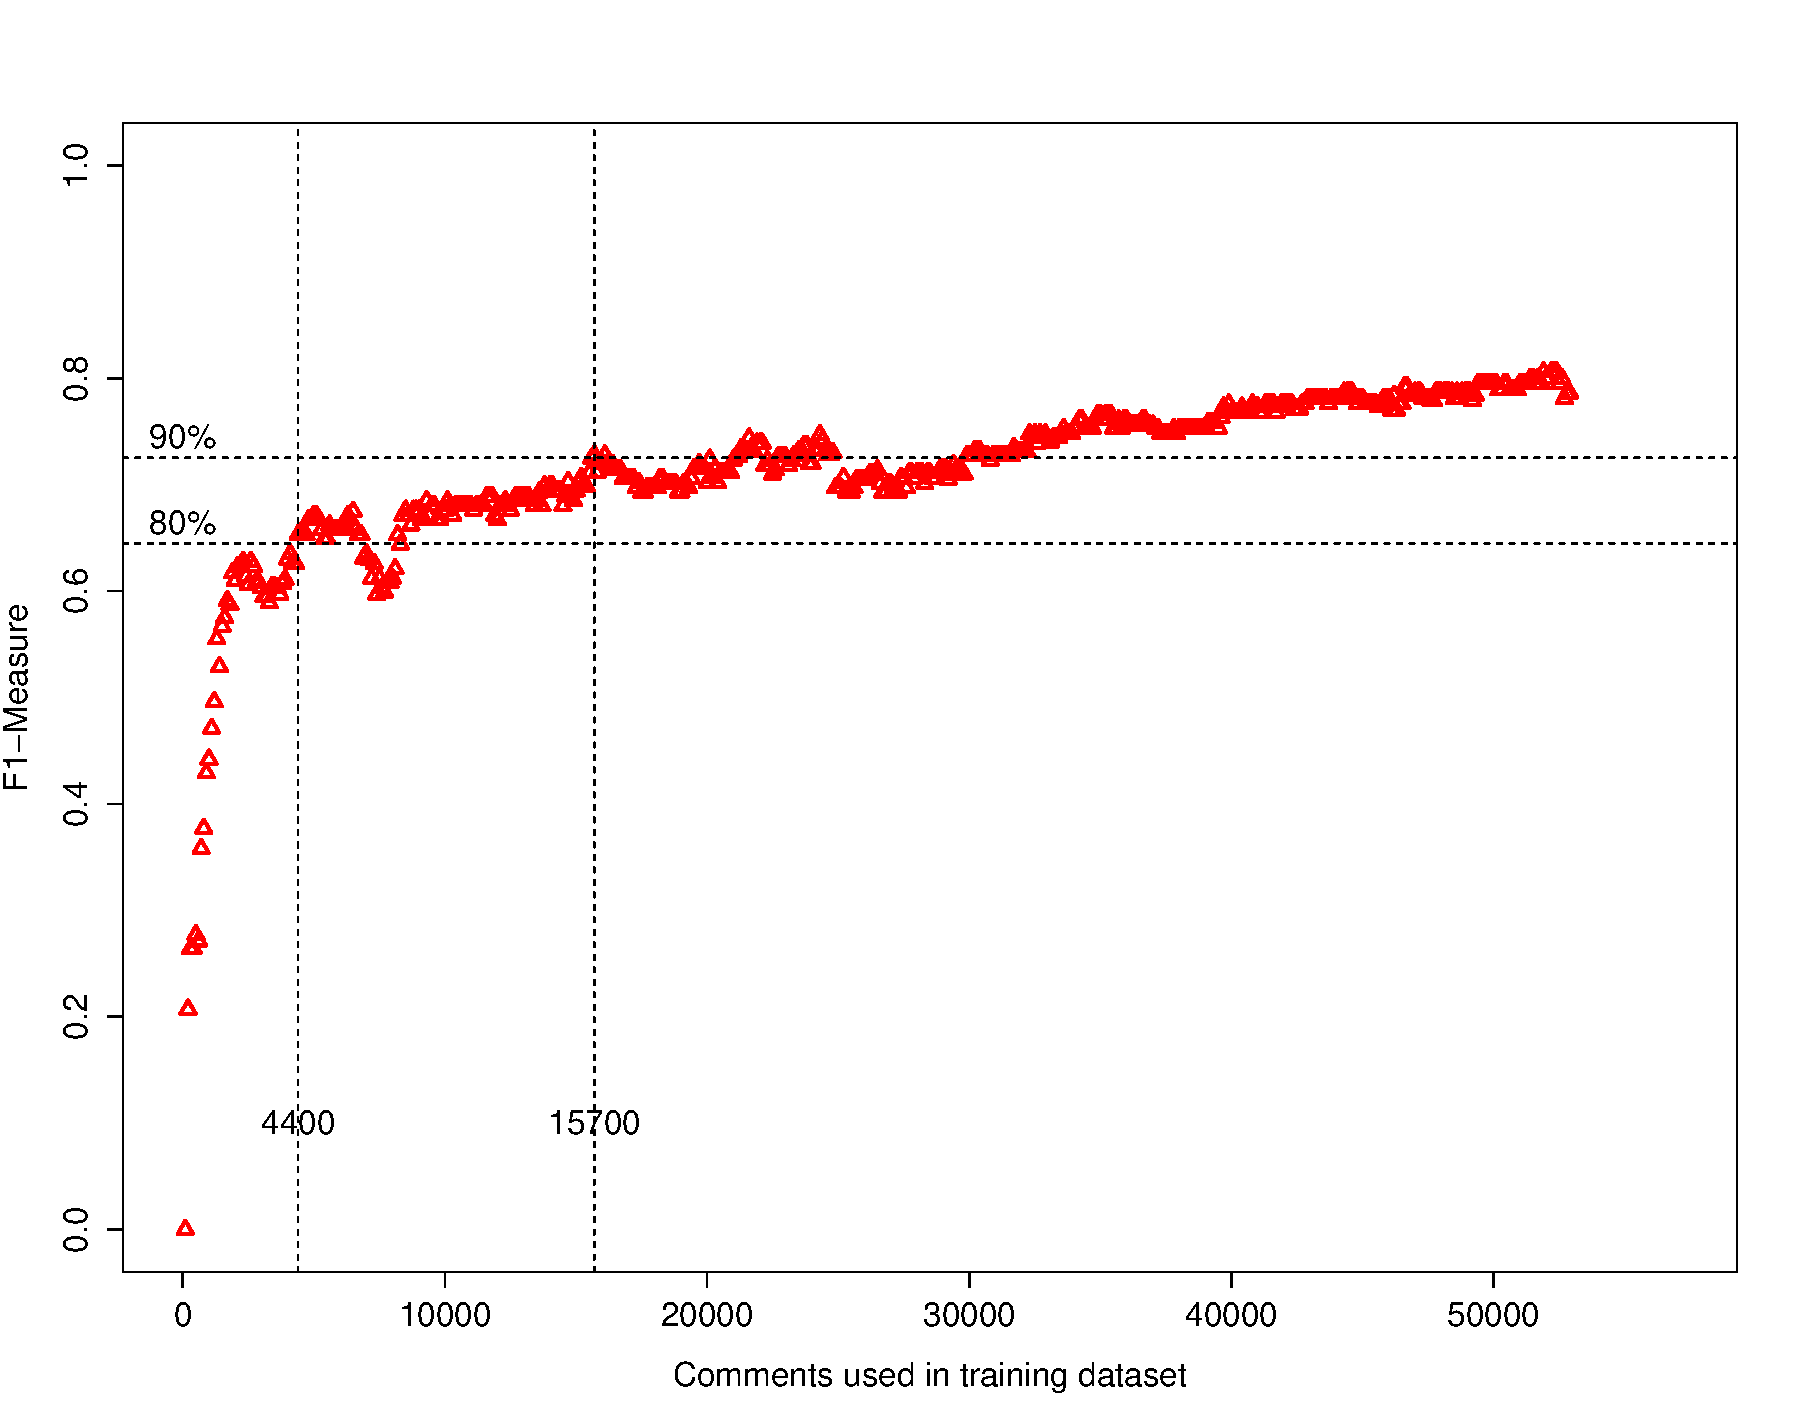
\includegraphics[width=0.49\textwidth]{figures/appendix/ten_fold_validation_requirement/ten_fold_validation_2_100.pdf}
  \vspace{-5mm}
  \caption{Ten Fold Validation Adding 100 Comments Per Time. Third Iteration}
  \label{fig:requirement_ten_fold_validation_2_100}
  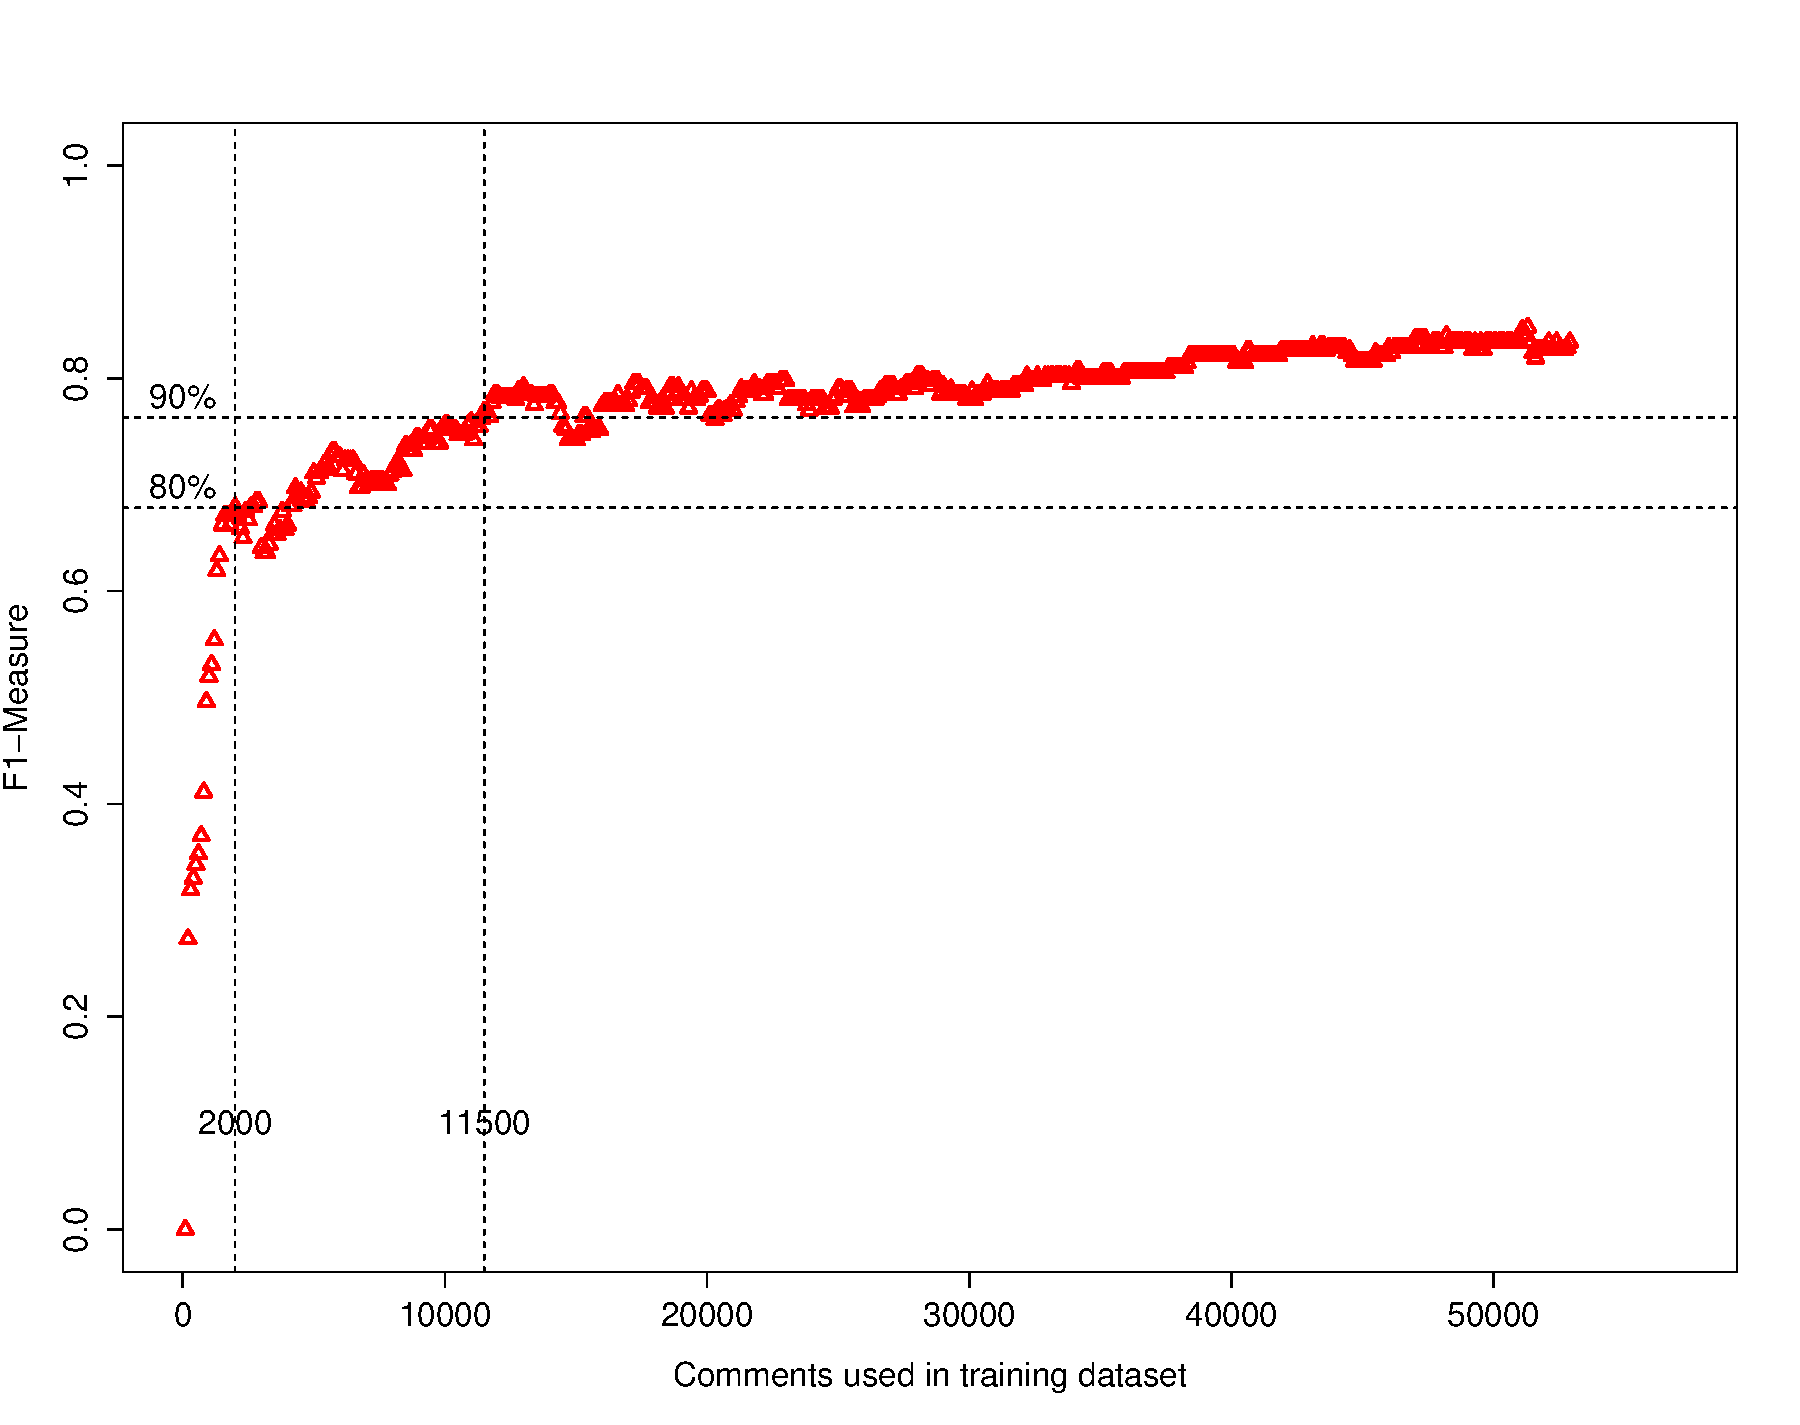
\includegraphics[width=0.49\textwidth]{figures/appendix/ten_fold_validation_requirement/ten_fold_validation_4_100.pdf}
  \vspace{-5mm}
  \caption{Ten Fold Validation Adding 100 Comments Per Time. Fifth Iteration}
  \label{fig:requirement_ten_fold_validation_4_100}
\end{figure}

\begin{figure}[thb!]
  \centering
  \vspace{-14mm}
  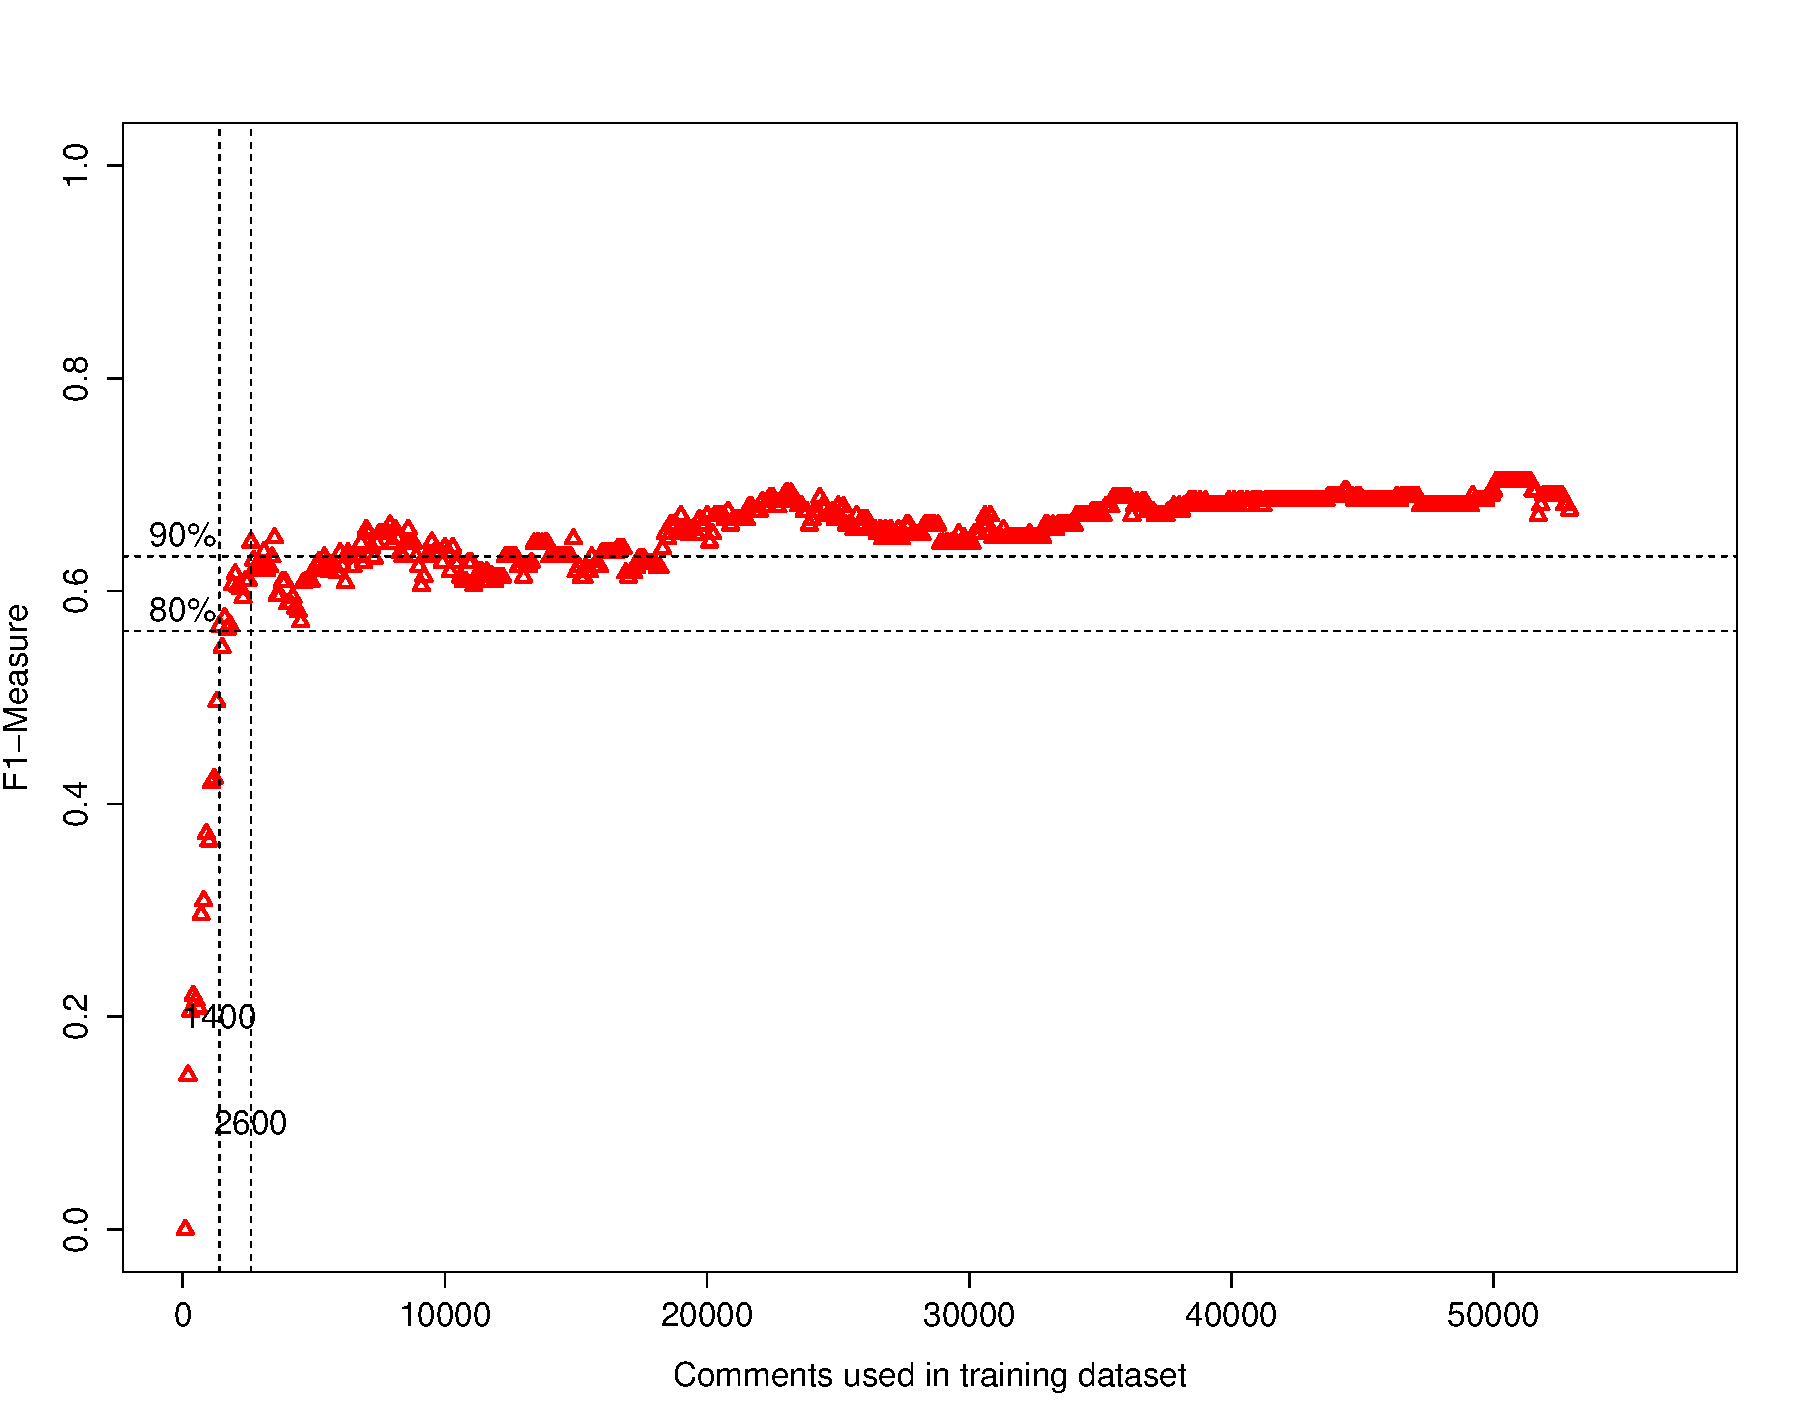
\includegraphics[width=0.49\textwidth]{figures/appendix/ten_fold_validation_requirement/ten_fold_validation_1_100.pdf}
  \vspace{-5mm}
  \caption{Ten Fold Validation Adding 100 Comments Per Time. Second Iteration}
  \label{fig:requirement_ten_fold_validation_1_100}
  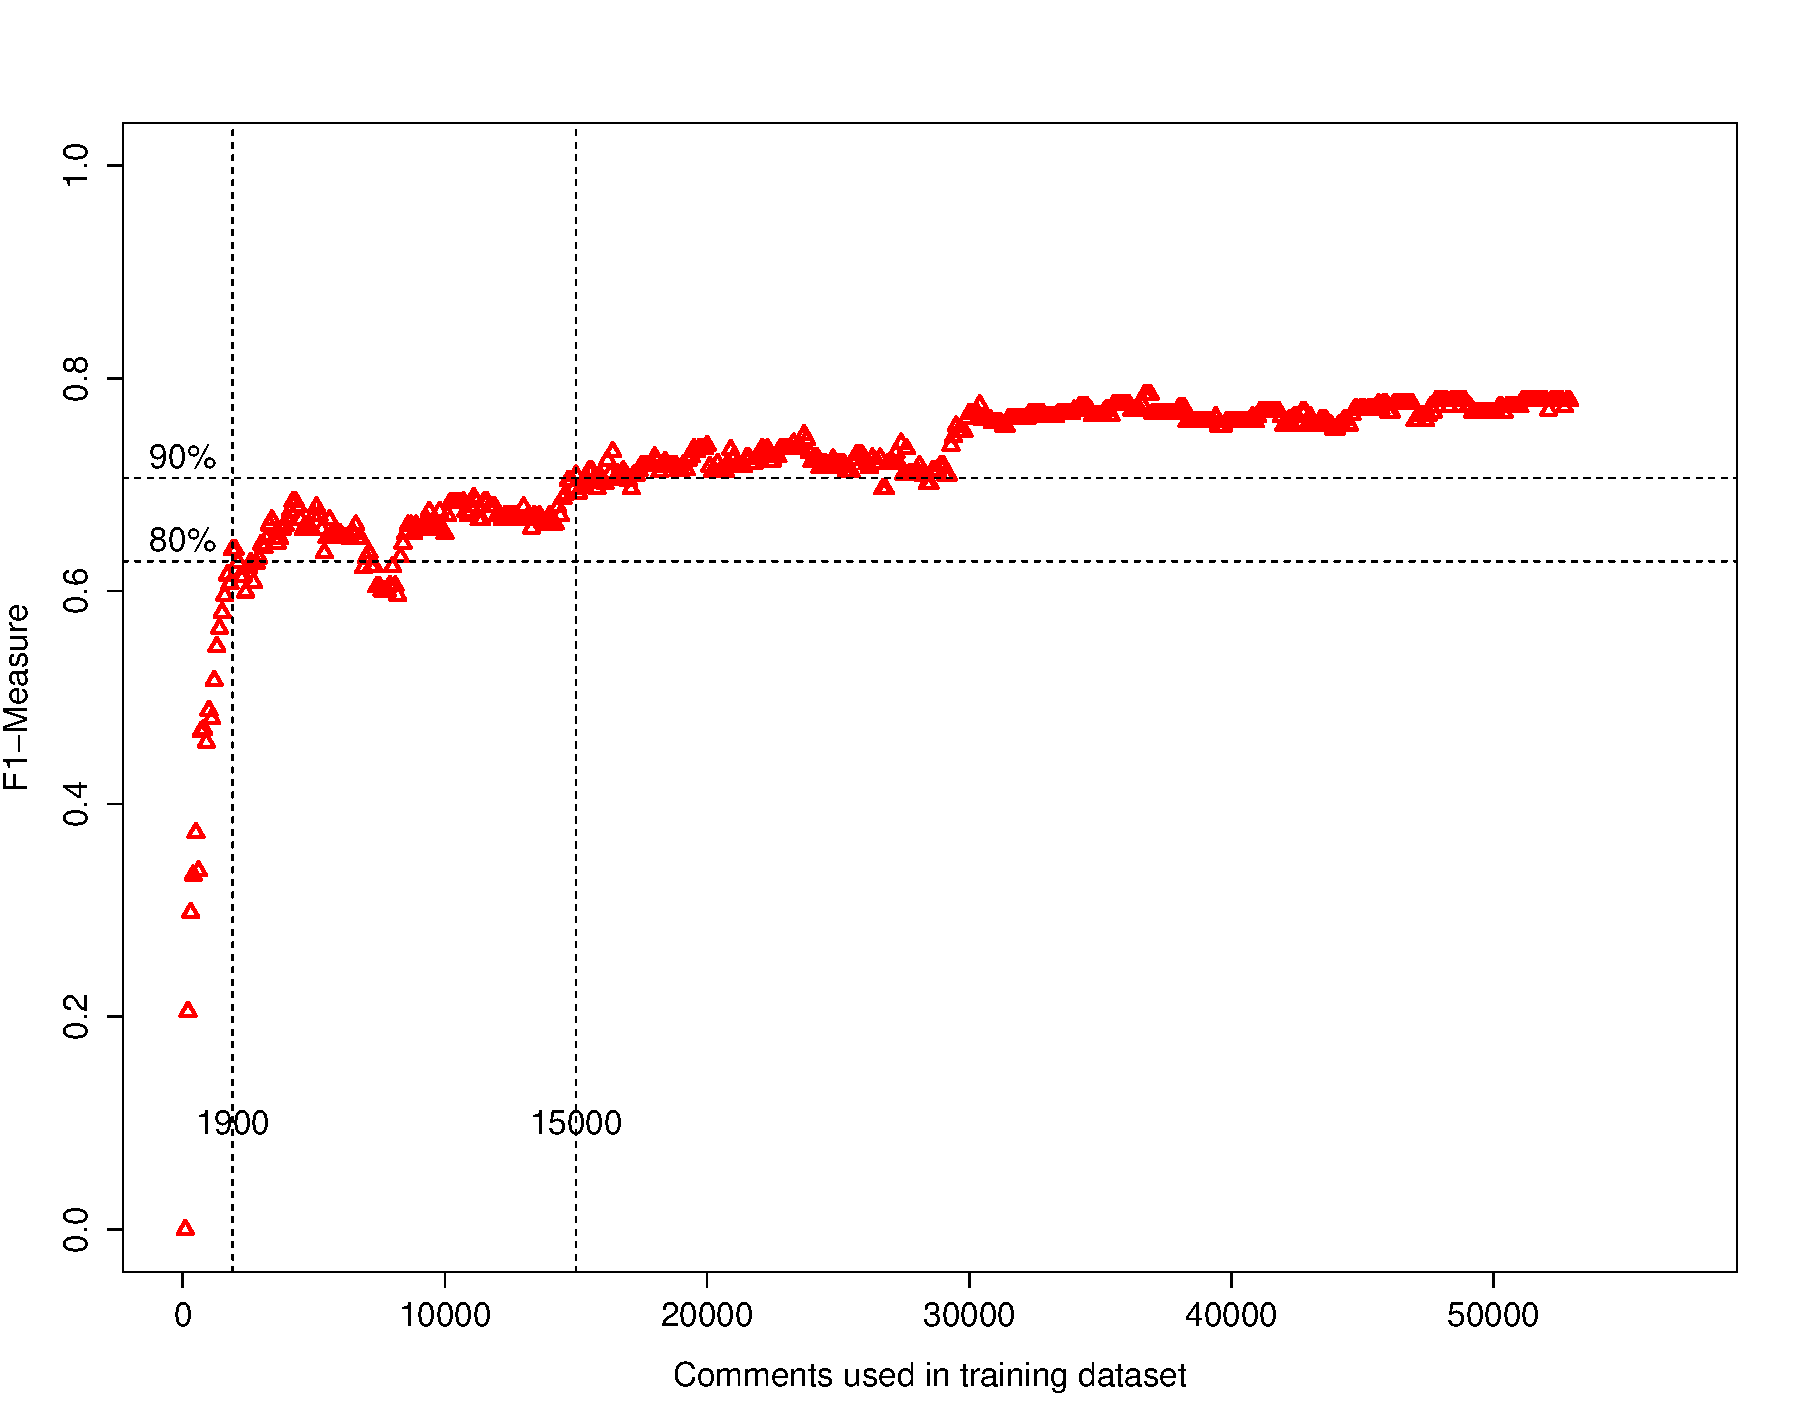
\includegraphics[width=0.49\textwidth]{figures/appendix/ten_fold_validation_requirement/ten_fold_validation_3_100.pdf}
  \vspace{-5mm}
  \caption{Ten Fold Validation Adding 100 Comments Per Time. Fourth Iteration}
  \label{fig:requirement_ten_fold_validation_3_100}
  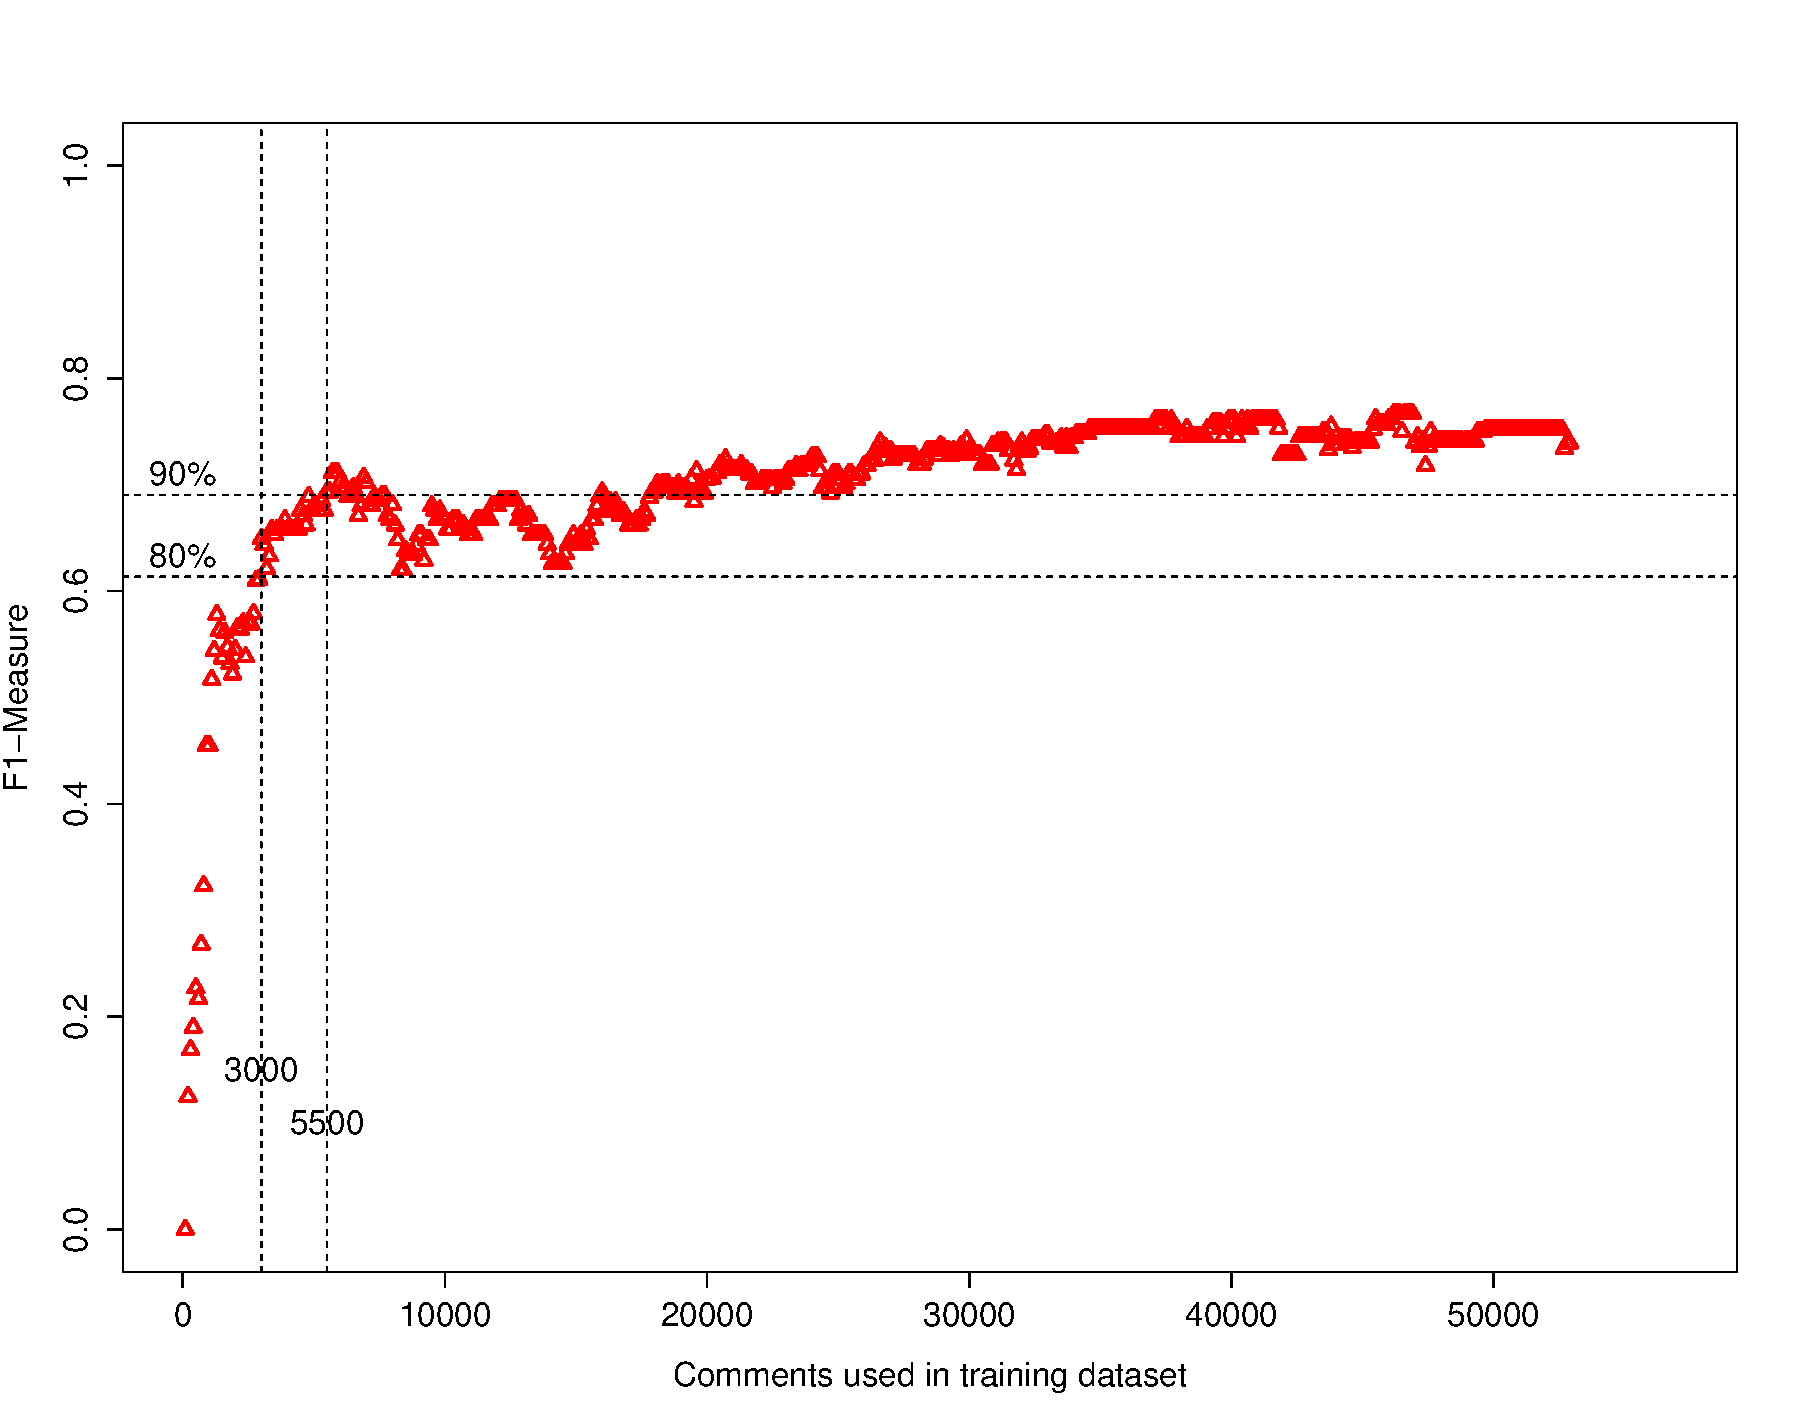
\includegraphics[width=0.49\textwidth]{figures/appendix/ten_fold_validation_requirement/ten_fold_validation_5_100.pdf}
  \vspace{-5mm}
  \caption{Ten Fold Validation Adding 100 Comments Per Time. Sixth Iteration}
  \label{fig:requirement_ten_fold_validation_5_100}
\end{figure}

\clearpage
\begin{figure}[thb!]
  \centering
  \vspace{-3mm}
  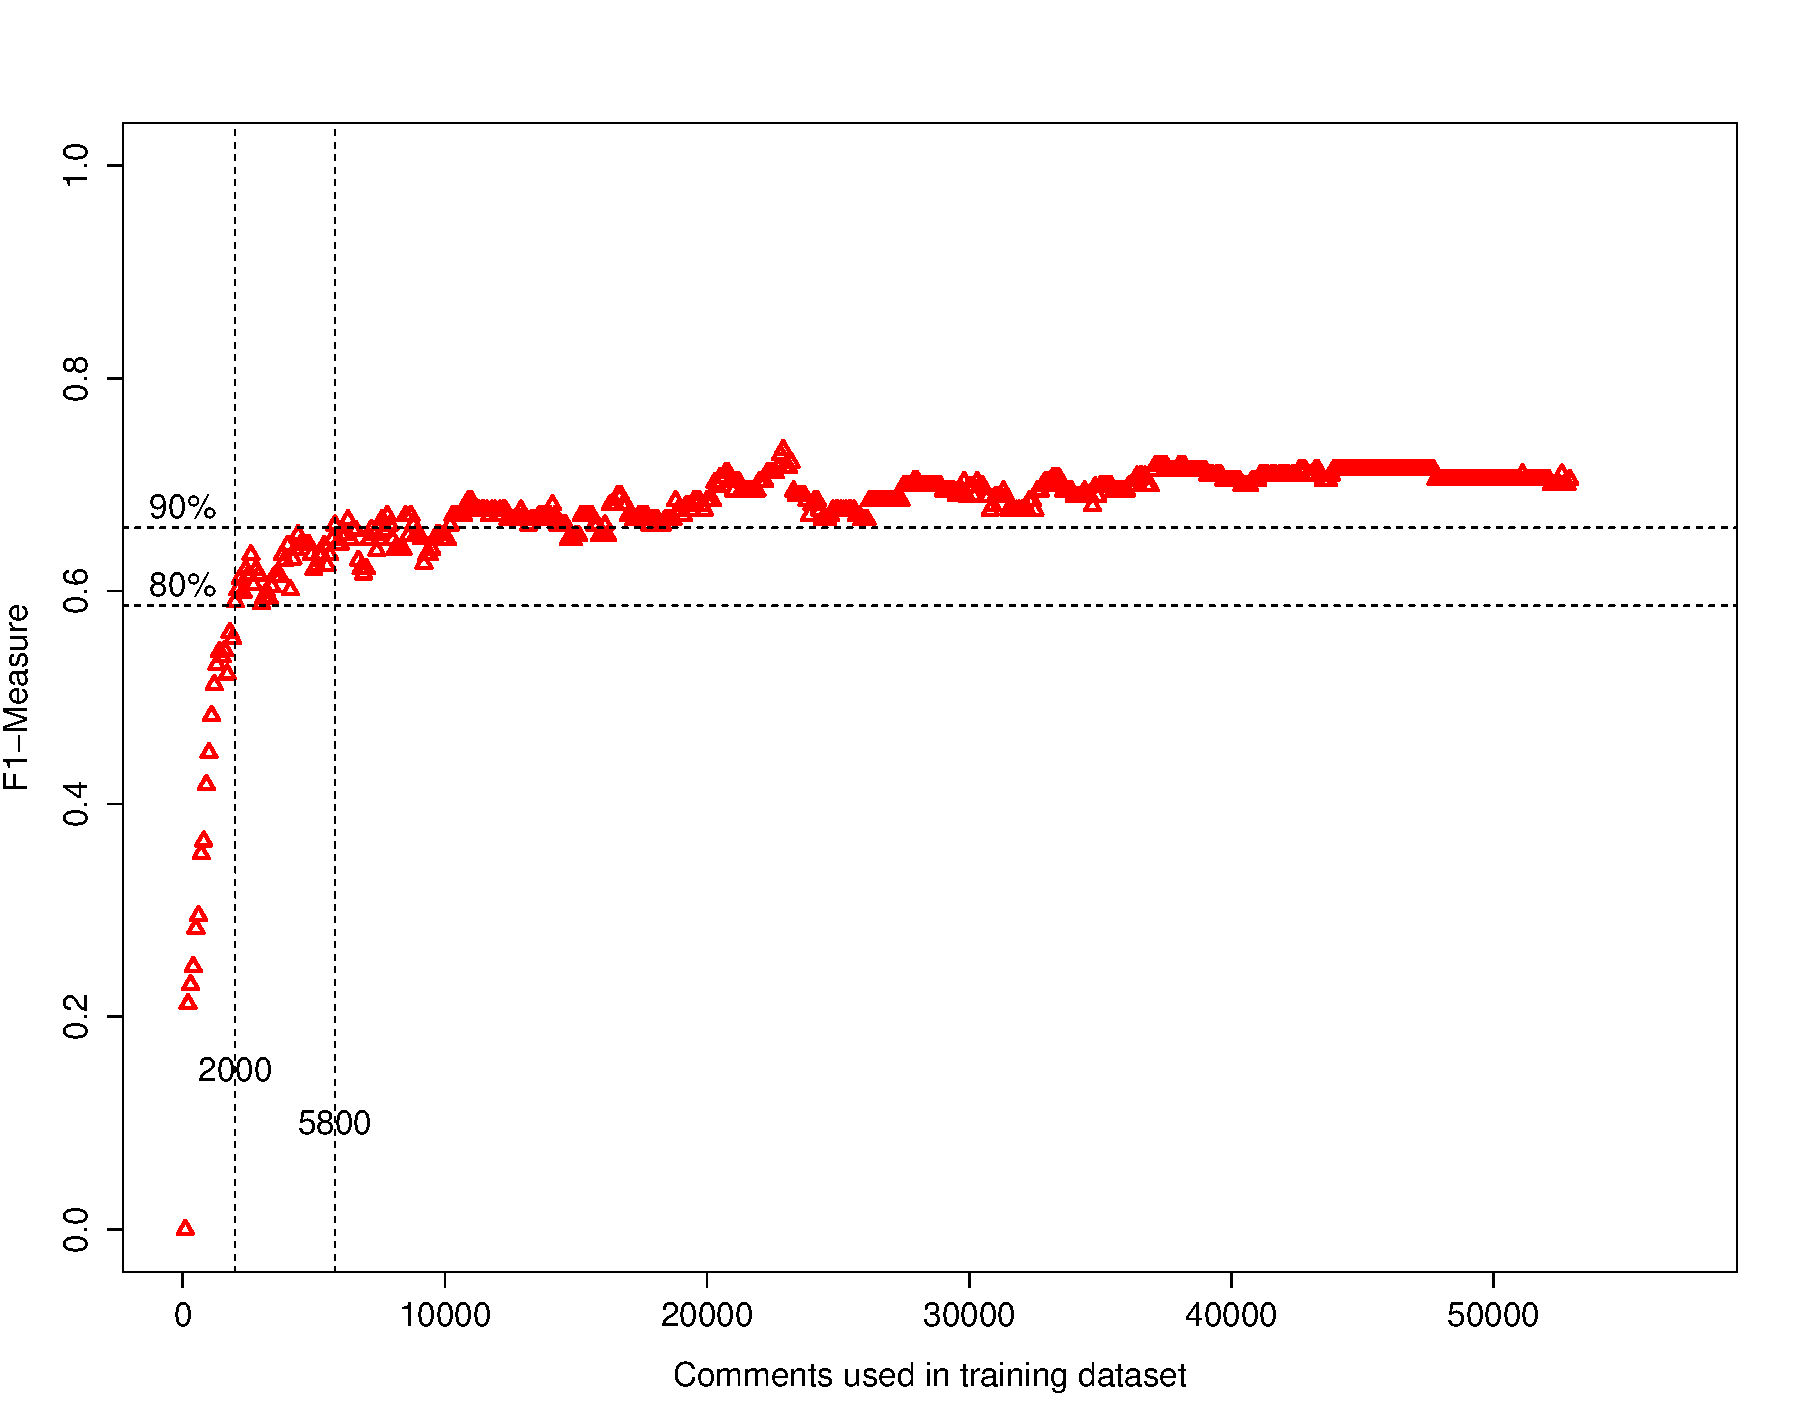
\includegraphics[width=0.49\textwidth]{figures/appendix/ten_fold_validation_requirement/ten_fold_validation_6_100.pdf}
  \vspace{-5mm}
  \caption{Ten Fold Validation Adding 100 Comments Per Time. Seventh Iteration}
  \label{fig:requirement_ten_fold_validation_6_100}
  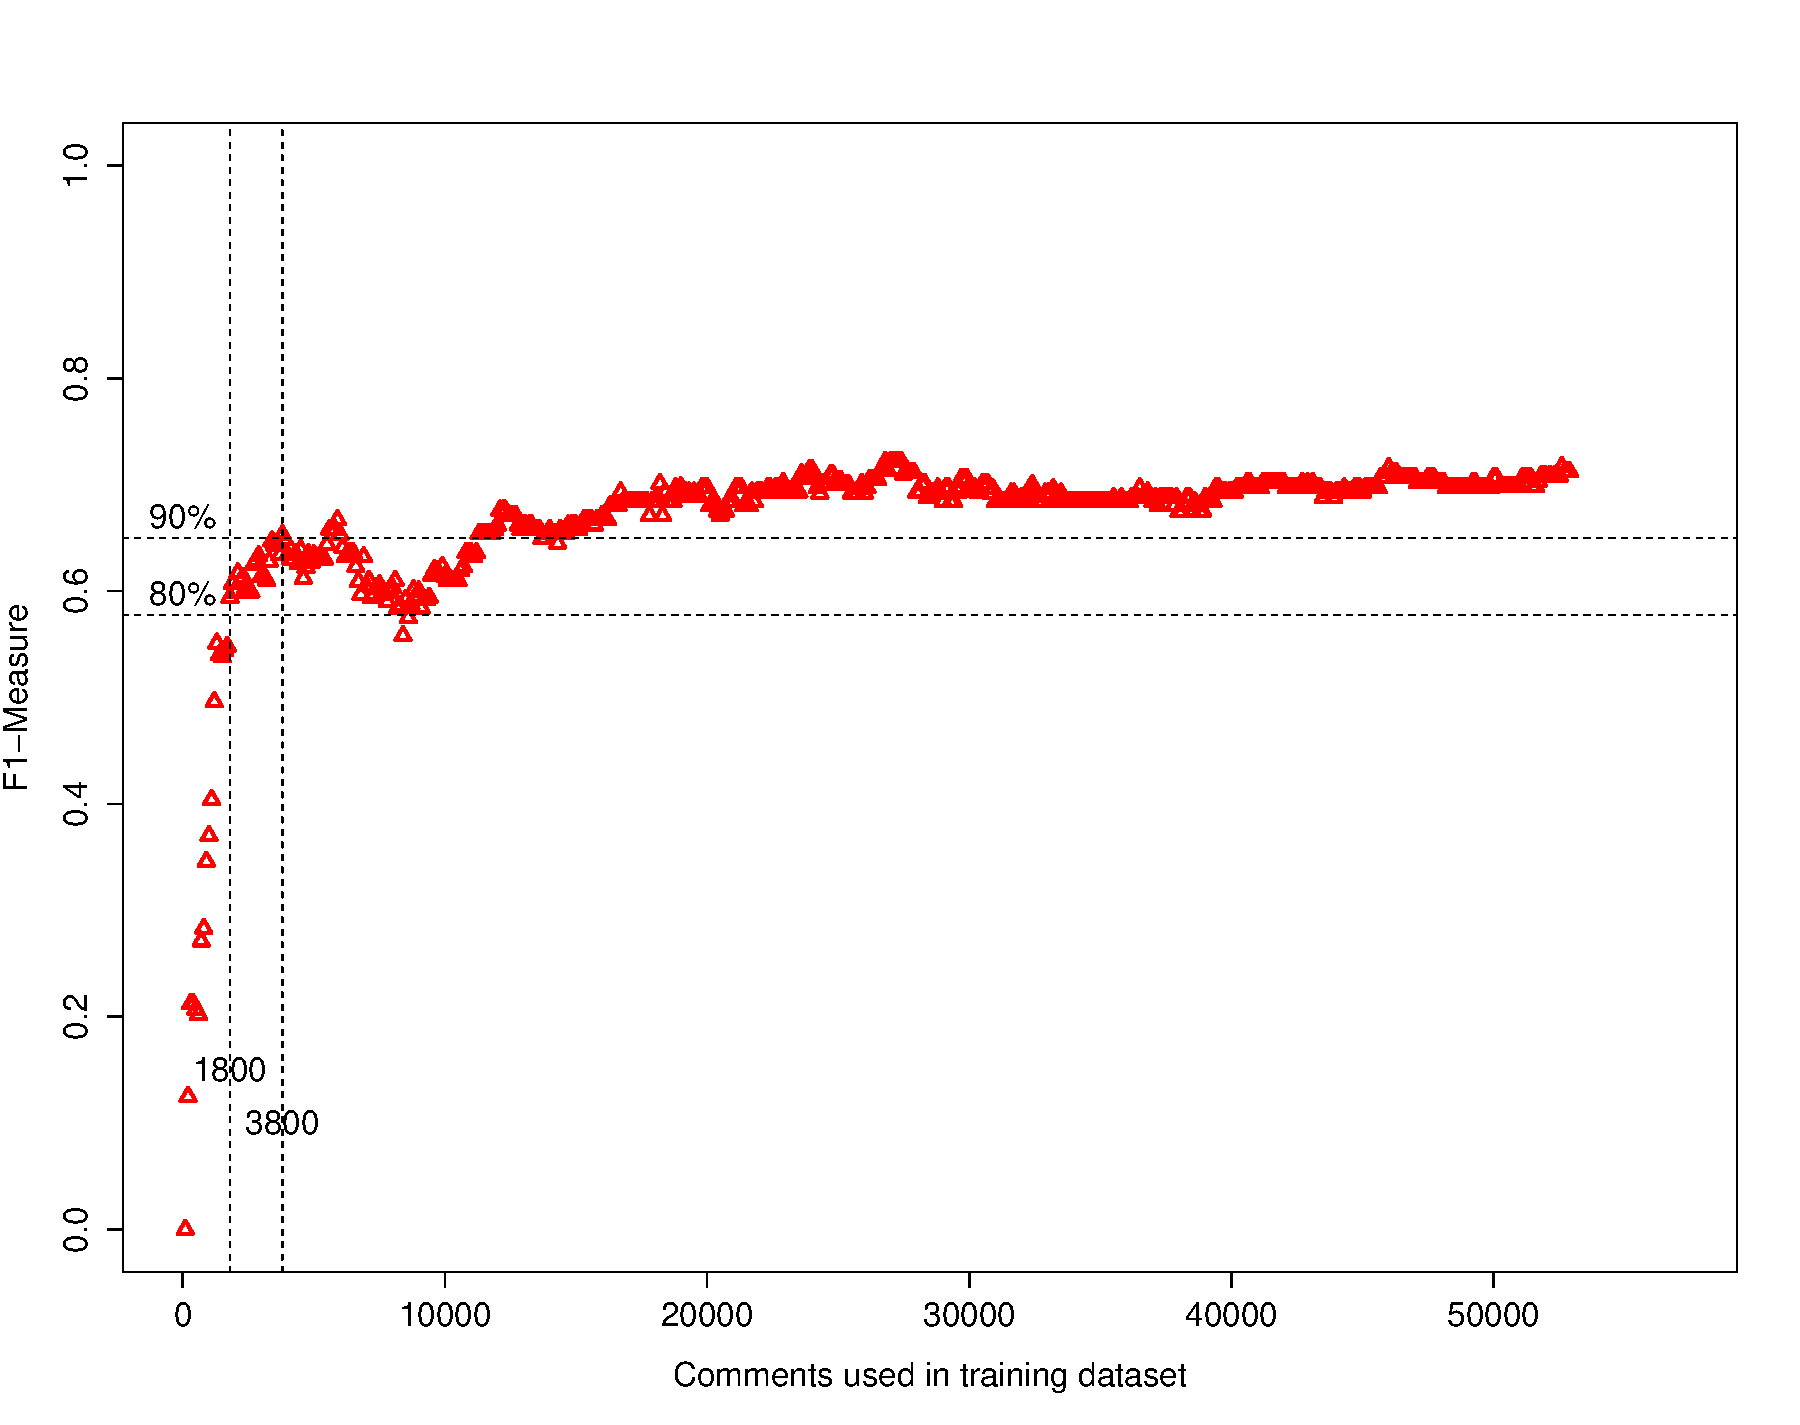
\includegraphics[width=0.49\textwidth]{figures/appendix/ten_fold_validation_requirement/ten_fold_validation_8_100.pdf}
  \vspace{-5mm}
  \caption{Ten Fold Validation Adding 100 Comments Per Time. Ninth Iteration}
  \label{fig:requirement_ten_fold_validation_8_100}
  \includegraphics[width=0.49\textwidth]{figures/appendix/ten_fold_validation_requirement/ten_fold_validation_average_100.pdf}
  \vspace{-5mm}
  \caption{Ten Fold Validation Adding 100 Comments Per Time. Average}
  \label{fig:requirement_ten_fold_validation_average_100}
\end{figure}

\begin{figure}[thb!]
  \centering
  \vspace{-93mm}
  \includegraphics[width=0.49\textwidth]{figures/appendix/ten_fold_validation_requirement/ten_fold_validation_7_100.pdf}
  \vspace{-5mm}
  \caption{Ten Fold Validation Adding 100 Comments Per Time. Eight Iteration}
  \label{fig:requirement_ten_fold_validation_7_100}
  \includegraphics[width=0.49\textwidth]{figures/appendix/ten_fold_validation_requirement/ten_fold_validation_9_100.pdf}
  \vspace{-5mm}
  \caption{Ten Fold Validation Adding 100 Comments Per Time. Tenth Iteration}
  \label{fig:requirement_ten_fold_validation_9_100}
  
\end{figure}

\clearpage
\begin{figure}[thb!]
  \centering
  \vspace{-3mm}
  \includegraphics[width=0.49\textwidth]{figures/appendix/ten_fold_validation_requirement/ten_fold_validation_0_500.pdf}
  \vspace{-5mm}
  \caption{Ten Fold Validation Adding 500 Comments Per Time. First Iteration}
  \label{fig:requirement_ten_fold_validation_0_100}
  \includegraphics[width=0.49\textwidth]{figures/appendix/ten_fold_validation_requirement/ten_fold_validation_2_500.pdf}
  \vspace{-5mm}
  \caption{Ten Fold Validation Adding 500 Comments Per Time. Third Iteration}
  \label{fig:requirement_ten_fold_validation_2_100}
  \includegraphics[width=0.49\textwidth]{figures/appendix/ten_fold_validation_requirement/ten_fold_validation_4_500.pdf}
  \vspace{-5mm}
  \caption{Ten Fold Validation Adding 500 Comments Per Time. Fifth Iteration}
  \label{fig:requirement_ten_fold_validation_4_100}
\end{figure}

\begin{figure}[thb!]
  \centering
  \vspace{-14mm}
  \includegraphics[width=0.49\textwidth]{figures/appendix/ten_fold_validation_requirement/ten_fold_validation_1_500.pdf}
  \vspace{-5mm}
  \caption{Ten Fold Validation Adding 500 Comments Per Time. Second Iteration}
  \label{fig:requirement_ten_fold_validation_1_100}
  \includegraphics[width=0.49\textwidth]{figures/appendix/ten_fold_validation_requirement/ten_fold_validation_3_500.pdf}
  \vspace{-5mm}
  \caption{Ten Fold Validation Adding 500 Comments Per Time. Fourth Iteration}
  \label{fig:requirement_ten_fold_validation_3_100}
  \includegraphics[width=0.49\textwidth]{figures/appendix/ten_fold_validation_requirement/ten_fold_validation_5_500.pdf}
  \vspace{-5mm}
  \caption{Ten Fold Validation Adding 500 Comments Per Time. Sixth Iteration}
  \label{fig:requirement_ten_fold_validation_5_100}
\end{figure}

\clearpage
\begin{figure}[thb!]
  \centering
  \vspace{-3mm}
  \includegraphics[width=0.49\textwidth]{figures/appendix/ten_fold_validation_requirement/ten_fold_validation_6_500.pdf}
  \vspace{-5mm}
  \caption{Ten Fold Validation Adding 500 Comments Per Time. Seventh Iteration}
  \label{fig:requirement_ten_fold_validation_6_100}
  \includegraphics[width=0.49\textwidth]{figures/appendix/ten_fold_validation_requirement/ten_fold_validation_8_500.pdf}
  \vspace{-5mm}
  \caption{Ten Fold Validation Adding 500 Comments Per Time. Ninth Iteration}
  \label{fig:requirement_ten_fold_validation_8_100}
  \includegraphics[width=0.49\textwidth]{figures/appendix/ten_fold_validation_requirement/ten_fold_validation_average_500.pdf}
  \vspace{-5mm}
  \caption{Ten Fold Validation Adding 500 Comments Per Time. Average}
  \label{fig:requirement_ten_fold_validation_average_100}
\end{figure}

\begin{figure}[thb!]
  \centering
  \vspace{-93mm}
  \includegraphics[width=0.49\textwidth]{figures/appendix/ten_fold_validation_requirement/ten_fold_validation_7_500.pdf}
  \vspace{-5mm}
  \caption{Ten Fold Validation Adding 500 Comments Per Time. Eight Iteration}
  \label{fig:requirement_ten_fold_validation_7_100}
  \includegraphics[width=0.49\textwidth]{figures/appendix/ten_fold_validation_requirement/ten_fold_validation_9_500.pdf}
  \vspace{-5mm}
  \caption{Ten Fold Validation Adding 500 Comments Per Time. Tenth Iteration}
  \label{fig:requirement_ten_fold_validation_9_100}
  
\end{figure}

% \clearpage
% \begin{table*}[!thb]
%     \begin{center}
%         \caption{Comparison of F1-measure Between the NLP-based, the Comment Patterns and the Random Baseline Approaches for Design and Requirement Debt}
%         \label{tbl:improvement_f1measure}
%         \begin{tabular}{l| c c c c c| c c c}
%         \toprule
        
%         % draw first line. The * centralizes the Project column, then set the total size of columns that we have
%         \multirow{4}{*}{\textbf{\thead{Project}}} & \multicolumn{5}{c|}{\textbf{\thead{Design debt}}} & \multicolumn{3}{c}{\textbf{\thead{Requirement debt}}} 
%         % indicates that from now on we are filling the content of the next line
%         \\ 
%         \cmidrule{2-6}
%         \cmidrule{7-9}
%         % remainder columns
%         & {\textbf{\thead{Our\\approach}}} & {\textbf{\thead{Comment\\patterns}}} & {\textbf{\thead{Revised\\comment p}}} & {\textbf{\thead{Improvement over\\comment patterns}}} & {\textbf{\thead{Improvement over\\revised comment p}}} & {\textbf{\thead{Our\\approach}}} & {\textbf{\thead{Revised \\comment p}}} & {\textbf{\thead{Improvement over\\revised comment p}}} \\
  
%         \midrule                                                  
%         \textbf{Ant}          &  0.517  &  0.175 & 0.237 &  2.9$\times$   &  2.1 $\times$   & 0.154  &  0.000  & -   \\
%         \textbf{ArgoUML}      &  0.814  &  0.078 & 0.107 &  10.4$\times$  &  7.6 $\times$   & 0.595  &  0.000  & -    \\
%         \textbf{Columba}      &  0.601  &  0.145 & 0.264 &  4.1$\times$   &  2.2 $\times$   & 0.804  &  0.117  & 6.8 $\times$  \\
%         \textbf{EMF}          &  0.470  &  0.114 & 0.231 &  4.1$\times$   &  2.0 $\times$   & 0.381  &  0.000  & -   \\
%         \textbf{Hibernate}    &  0.744  &   0.15 & 0.227 &  4.9$\times$   &  3.2 $\times$   & 0.476  &  0.000  & -   \\
%         \textbf{JEdit}        &  0.509  &  0.324 & 0.342 &  1.5$\times$   &  1.4 $\times$   & 0.091  &  0.000  & -   \\
%         \textbf{JFreeChart}   &  0.492  &  0.053 & 0.282 &  9.2$\times$   &  1.7 $\times$   & 0.321  &  0.000  & -   \\
%         \textbf{Jmeter}       &  0.731  &  0.127 & 0.194 &  5.7$\times$   &  3.7 $\times$   & 0.237  &  0.148  & 1.6 $\times$  \\
%         \textbf{JRuby}        &  0.783  &  0.138 & 0.620 &  5.6$\times$   &  1.2 $\times$   & 0.435  &  0.409  & 1.0 $\times$   \\
%         \textbf{SQuirrel}     &  0.540  &  0.071 & 0.175 &  7.6$\times$   &  3.0 $\times$   & 0.541  &  0.000  & -   \\
%         \midrule 
%         \textbf{Average}      &  0.620  & 0.137  & 0.267 &  4.5$\times$   & 2.3  $\times$   & 0.403  &  0.067  & 5.9 $\times$  \\ 
%         \bottomrule
%         \end{tabular}
%     \end{center}    
% \end{table*}


\clearpage
\begin{table}[h]
  \begin{minipage}{\textwidth}
    \begin{center}
        \caption{Detailed NLP-based Approach Performance Considering Different Types of Self-admitted Technical Debt}
        \label{tbl:detailed_nlpbased_performance_comparison}
        \begin{tabular}{l| c c c}
        \toprule
        
        \textbf{\thead{Project}} & \textbf{\thead{Precision}} & \textbf{\thead{Recall}} & \textbf{\thead{F1 measure}} \\
        \midrule
        \textbf{Ant}           &  0.547 & 0.481 &  0.512 \\
        \textbf{ArgoUML}       &  0.822 & 0.815 &  0.819 \\
        \textbf{Columba}       &  0.754 & 0.746 &  0.750 \\
        \textbf{EMF}           &  0.581 & 0.383 &  0.462 \\
        \textbf{Hibernate}     &  0.844 & 0.697 &  0.763 \\
        \textbf{JEdit}         &  0.745 & 0.333 &  0.461 \\
        \textbf{JFreeChart}    &  0.611 & 0.442 &  0.513 \\
        \textbf{Jmeter}        &  0.727 & 0.703 &  0.715 \\
        \textbf{JRuby}         &  0.801 & 0.746 &  0.773 \\
        \textbf{SQuirrel}      &  0.641 & 0.552 &  0.593 \\
        \bottomrule
        \end{tabular}
    \end{center}
  \end{minipage}    
\end{table}

% \begin{table}[!thb]
%     \begin{center}
%         \caption{Top Ten Textual Features Used to Identify Design and Requirement Self-Admitted Technical Debt}
%         \label{tbl:top_ten_features}
%         \begin{tabular}{l| l l| l }
%         \toprule
%         \textbf{Rank} & \textbf{Design Debt} & \textbf{Requirement Debt}  & \textbf{Technical Debt}\\
%         \midrule
%          \textbf{1}  & hack       &   todo            & hack         \\
%          \textbf{2}  & workaround &   needed          & workaround   \\
%          \textbf{3}  & yuck!      &   implementation  & yuck!        \\
%          \textbf{4}  & kludge     &   fixme           & kludge       \\
%          \textbf{5}  & stupidity  &   xxx             & stupidity    \\
%          \textbf{6}  & needed?    &   ends?           & needed?      \\
%          \textbf{7}  & columns?   &   convention      & unused?      \\
%          \textbf{8}  & unused?    &   configurable    & fixme        \\
%          \textbf{9}  & wtf?       &   apparently      & todo         \\
%          \textbf{10} & todo       &   fudging         & wtf?         \\
%         \bottomrule
%         \end{tabular}
%     \end{center}    
% \end{table}

% Cls TECHNICAL_DEBT: TP=52  FN=56  FP=43  TN=3924;  Acc 0.976 P 0.547 R 0.481 F1 0.512
% Cls TECHNICAL_DEBT: TP=988 FN=224 FP=214 TN=7801;  Acc 0.953 P 0.822 R 0.815 F1 0.819
% Cls TECHNICAL_DEBT: TP=126 FN=43  FP=41  TN=6218;  Acc 0.987 P 0.754 R 0.746 F1 0.750
% Cls TECHNICAL_DEBT: TP=36  FN=58  FP=26  TN=4245;  Acc 0.981 P 0.581 R 0.383 F1 0.462
% Cls TECHNICAL_DEBT: TP=292 FN=127 FP=54  TN=2441;  Acc 0.938 P 0.844 R 0.697 F1 0.763
% Cls TECHNICAL_DEBT: TP=70  FN=140 FP=24  TN=10040; Acc 0.984 P 0.745 R 0.333 F1 0.461
% Cls TECHNICAL_DEBT: TP=88  FN=111 FP=56  TN=4142;  Acc 0.962 P 0.611 R 0.442 F1 0.513
% Cls TECHNICAL_DEBT: TP=237 FN=100 FP=89  TN=7581;  Acc 0.976 P 0.727 R 0.703 F1 0.715
% Cls TECHNICAL_DEBT: TP=338 FN=115 FP=84  TN=4191;  Acc 0.958 P 0.801 R 0.746 F1 0.773
% Cls TECHNICAL_DEBT: TP=143 FN=116 FP=80  TN=6828;  Acc 0.973 P 0.641 R 0.552 F1 0.593





